%%____________________________________________________________________________||
\clearpage
\section{``Lost lepton'' background estimation}
\label{app:ttw}

\subsection{PU reweighting}

\begin{figure}[!h]
  \centering
  \subfigure[PU weight up variation]{
    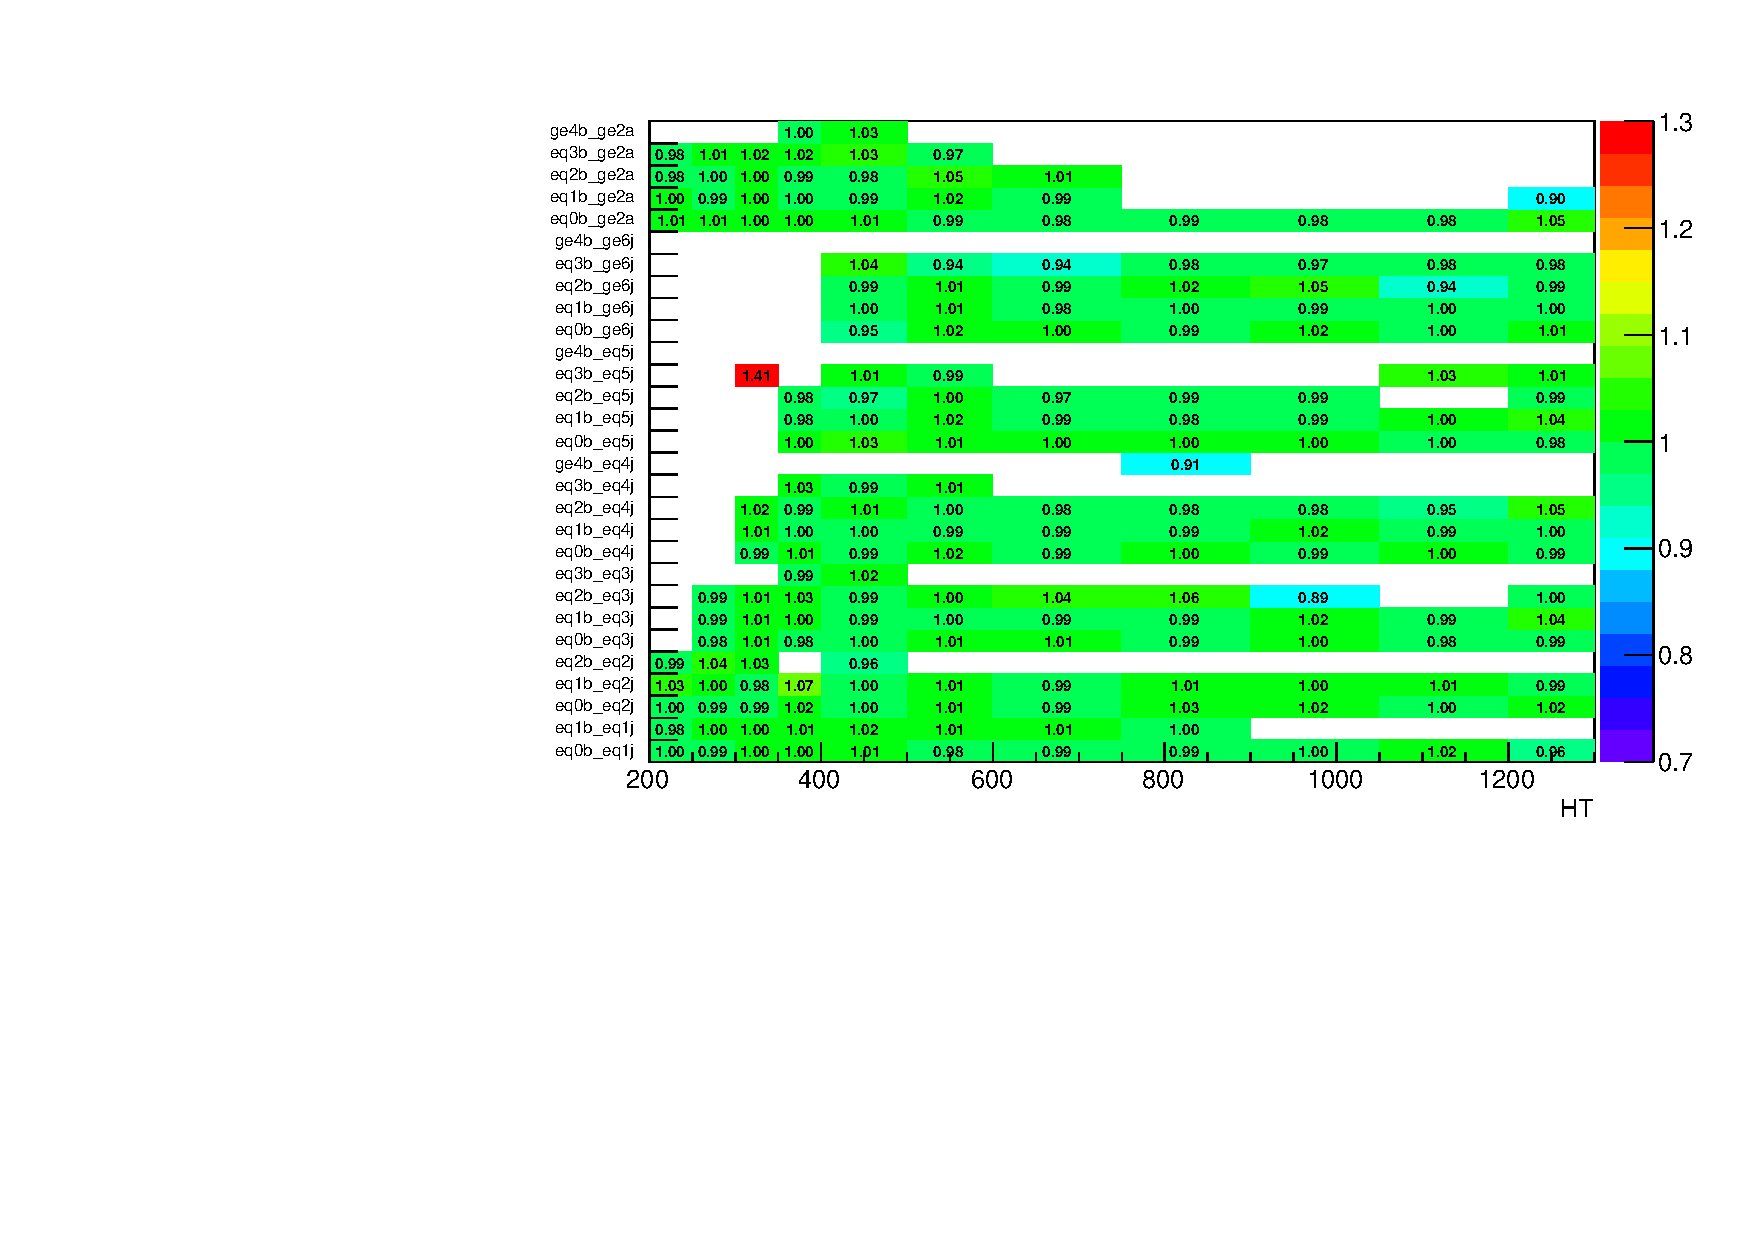
\includegraphics[width=0.5\textwidth]{figures/mcSystematics36p4fb/Ttw/mu/ratiotfh_ht_mht_allpuWeight_Up.pdf}
  } ~~
  \subfigure[PU weight down variation]{
    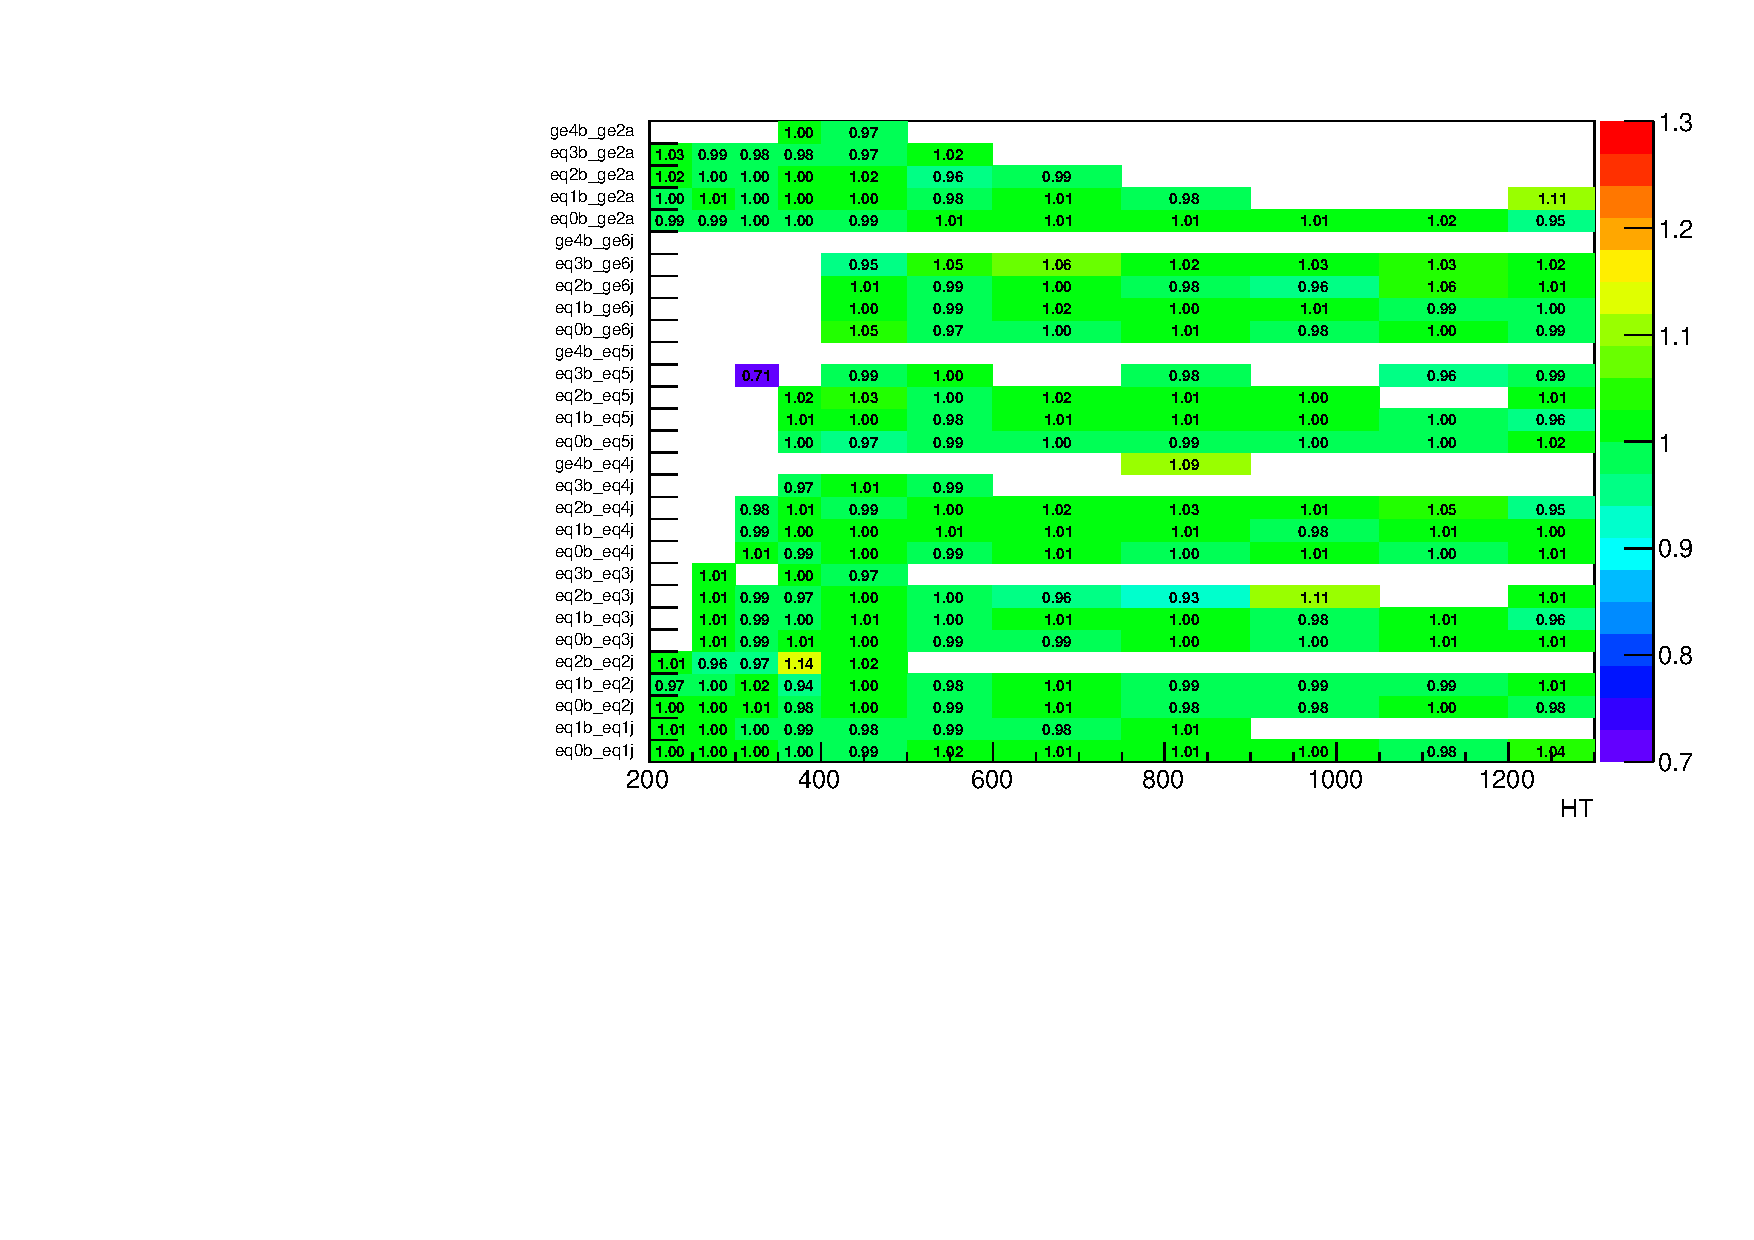
\includegraphics[width=0.5\textwidth]{figures/mcSystematics36p4fb/Ttw/mu/ratiotfh_ht_mht_allpuWeight_Down.pdf}
  }\\

  \caption{\label{fig:tfSyst_pu_muToTtw} The relative change in the $\mj \rightarrow \mathrm{tt+W}$ transfer
  factors when varying PU weight in MC within its uncertainties, as a function of \scalht and jet category. 
  Variations corresponding to $+1\sigma$ ($-1\sigma$) are shown in the left (right) figure. 
  }
\end{figure}

\subsection{Signal trigger efficiency}

\begin{figure}[!h]
  \centering
  \subfigure[trigger weight up variation]{
    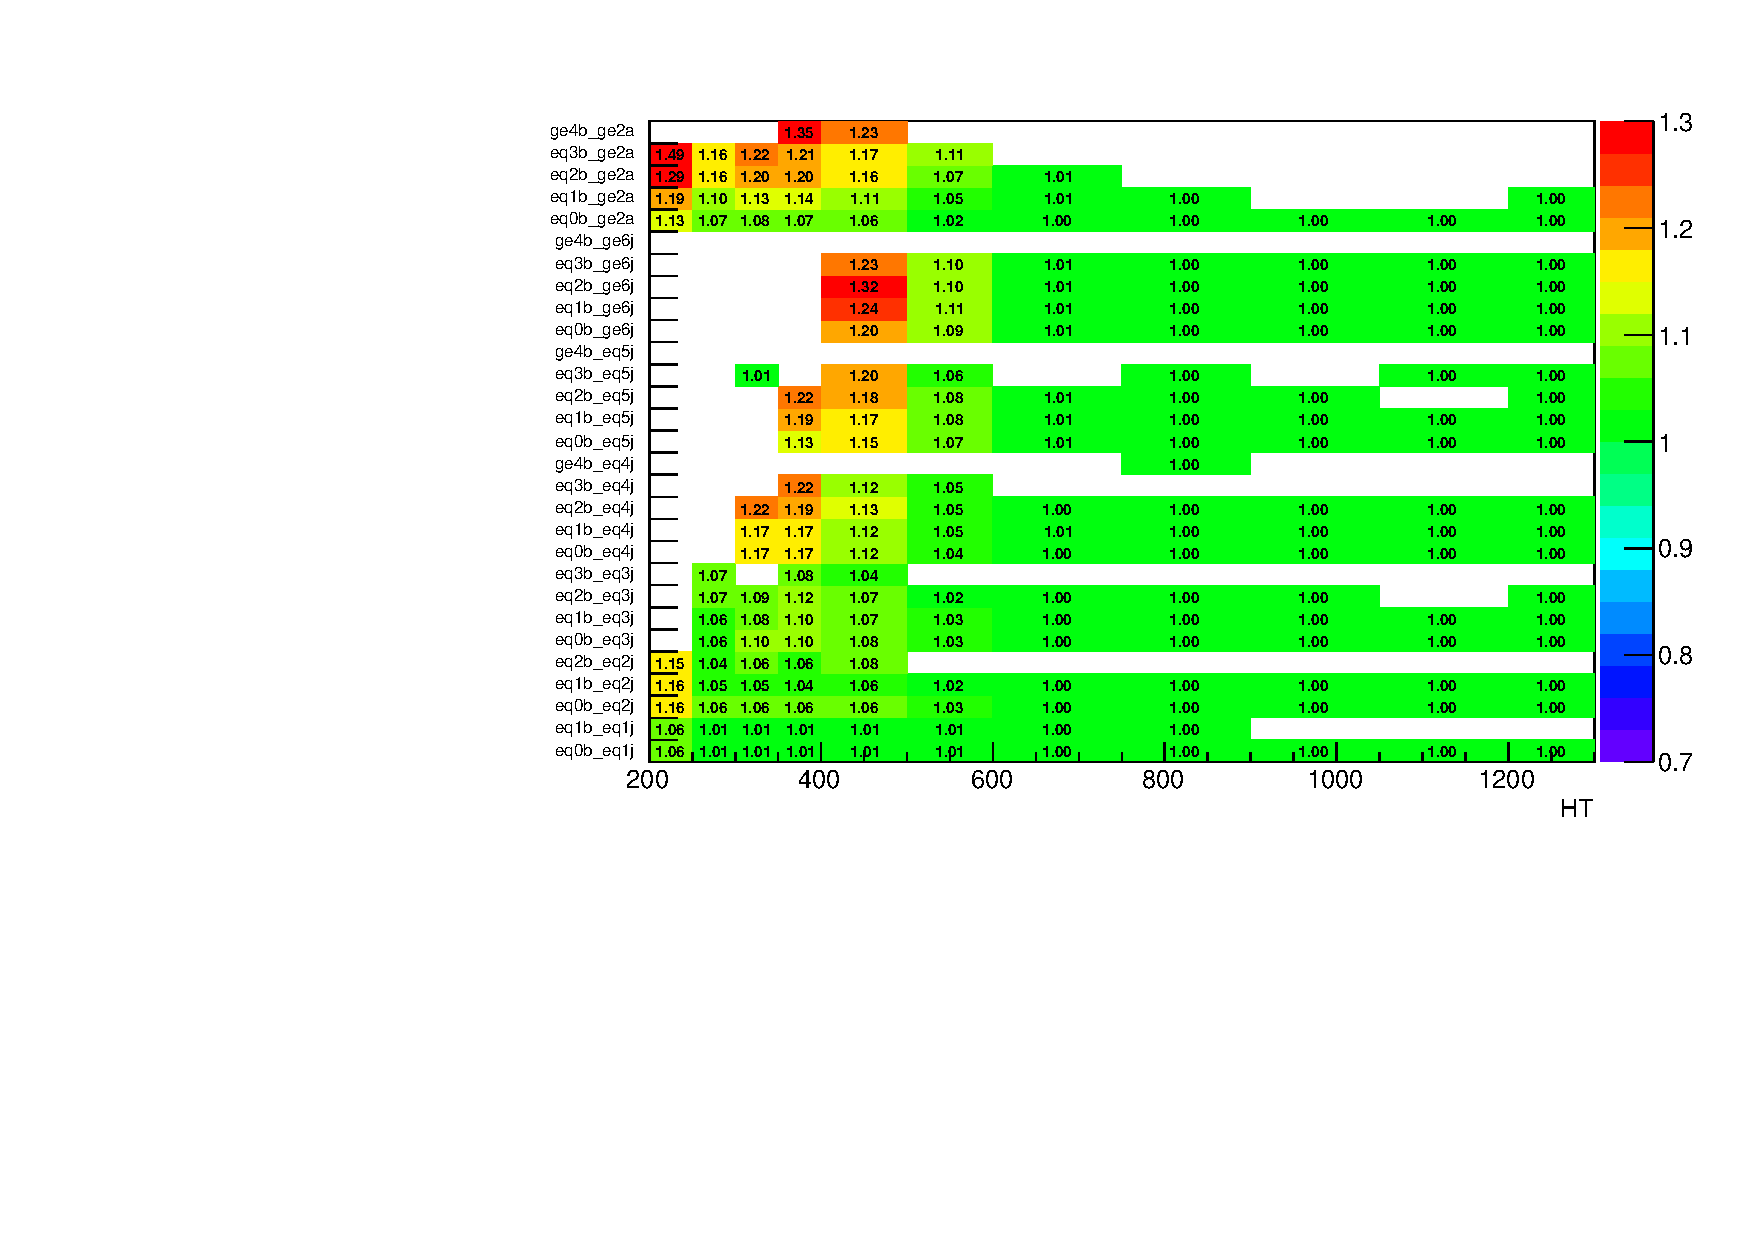
\includegraphics[width=0.5\textwidth]{figures/mcSystematics36p4fb/Ttw/mu/ratiotfh_ht_mht_alltriggerWeight_Up.pdf}
  } ~~
  \subfigure[trigger weight down variation]{
    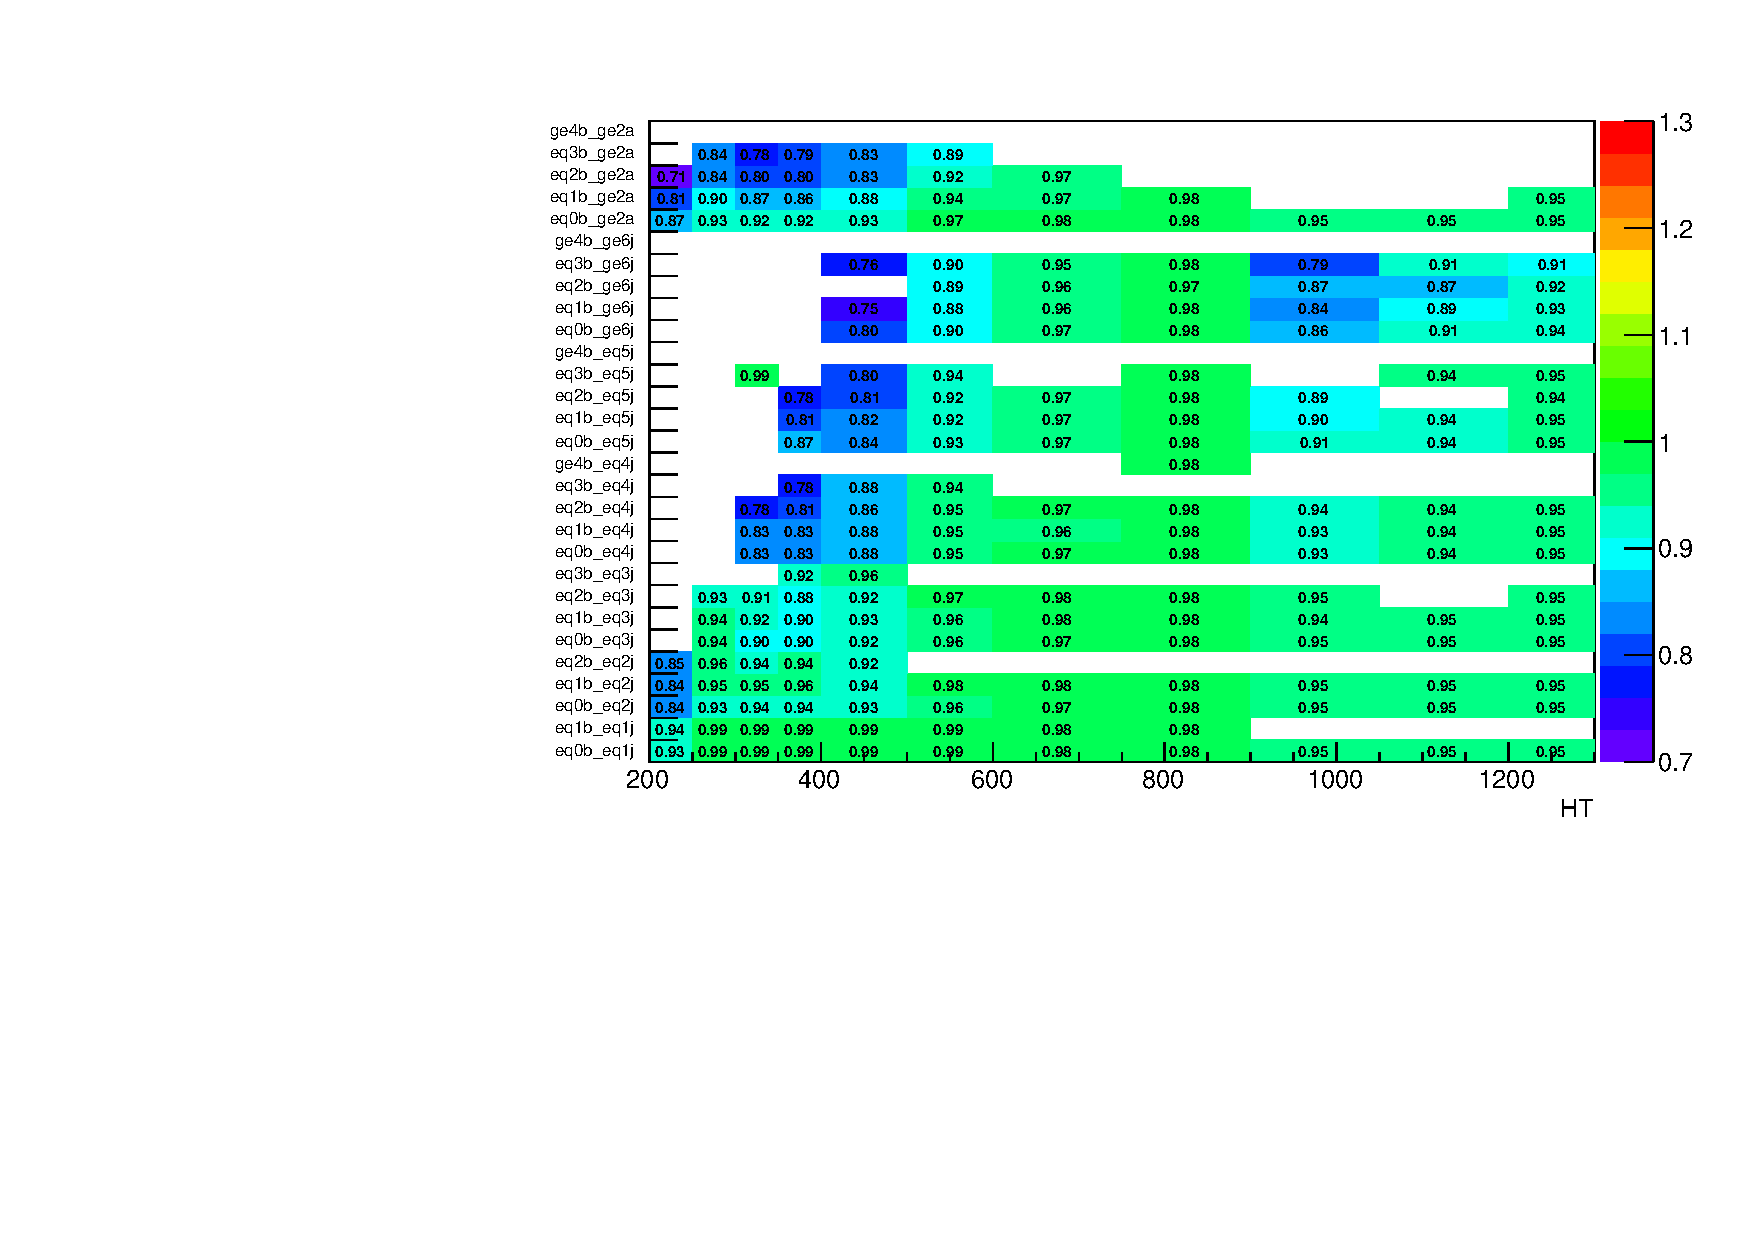
\includegraphics[width=0.5\textwidth]{figures/mcSystematics36p4fb/Ttw/mu/ratiotfh_ht_mht_alltriggerWeight_Down.pdf}
  }\\

  \caption{\label{fig:tfSyst_trigger_muToTtw} The relative change in the $\mj \rightarrow \mathrm{tt+W}$ transfer
  factors when varying trigger weight in MC within its uncertainties, as a function of \scalht and jet category. 
  Variations corresponding to $+1\sigma$ ($-1\sigma$) are shown in the left (right) figure. 
  }
\end{figure}

\clearpage
\subsection{Lepton trigger / identification / isolation efficiency}

\begin{figure}[!h]
  \centering
  \subfigure[muon scale factor up variation]{
    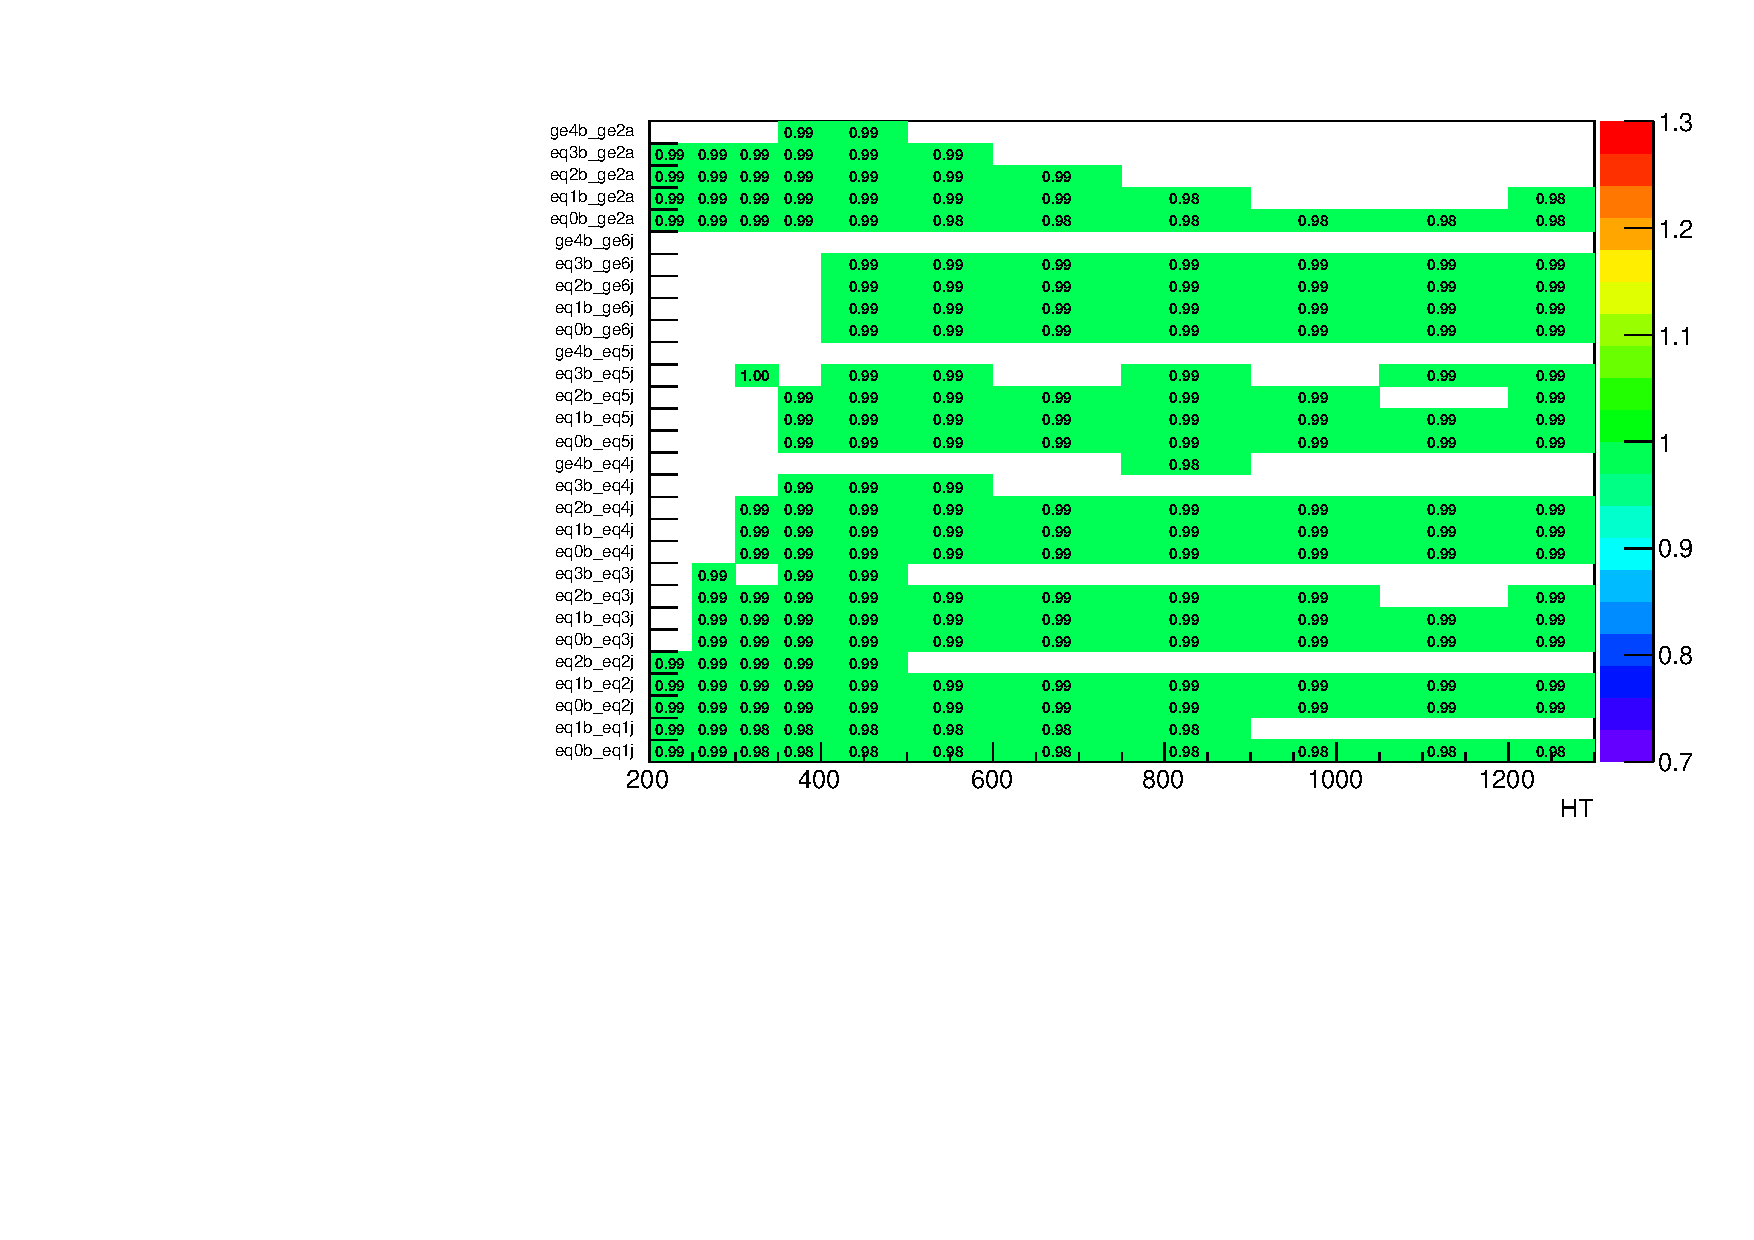
\includegraphics[width=0.5\textwidth]{figures/mcSystematics36p4fb/Ttw/mu/ratiotfh_ht_mht_allmuonSfWeight_Up.pdf}
  } ~~
  \subfigure[muon scale factor down variation]{
    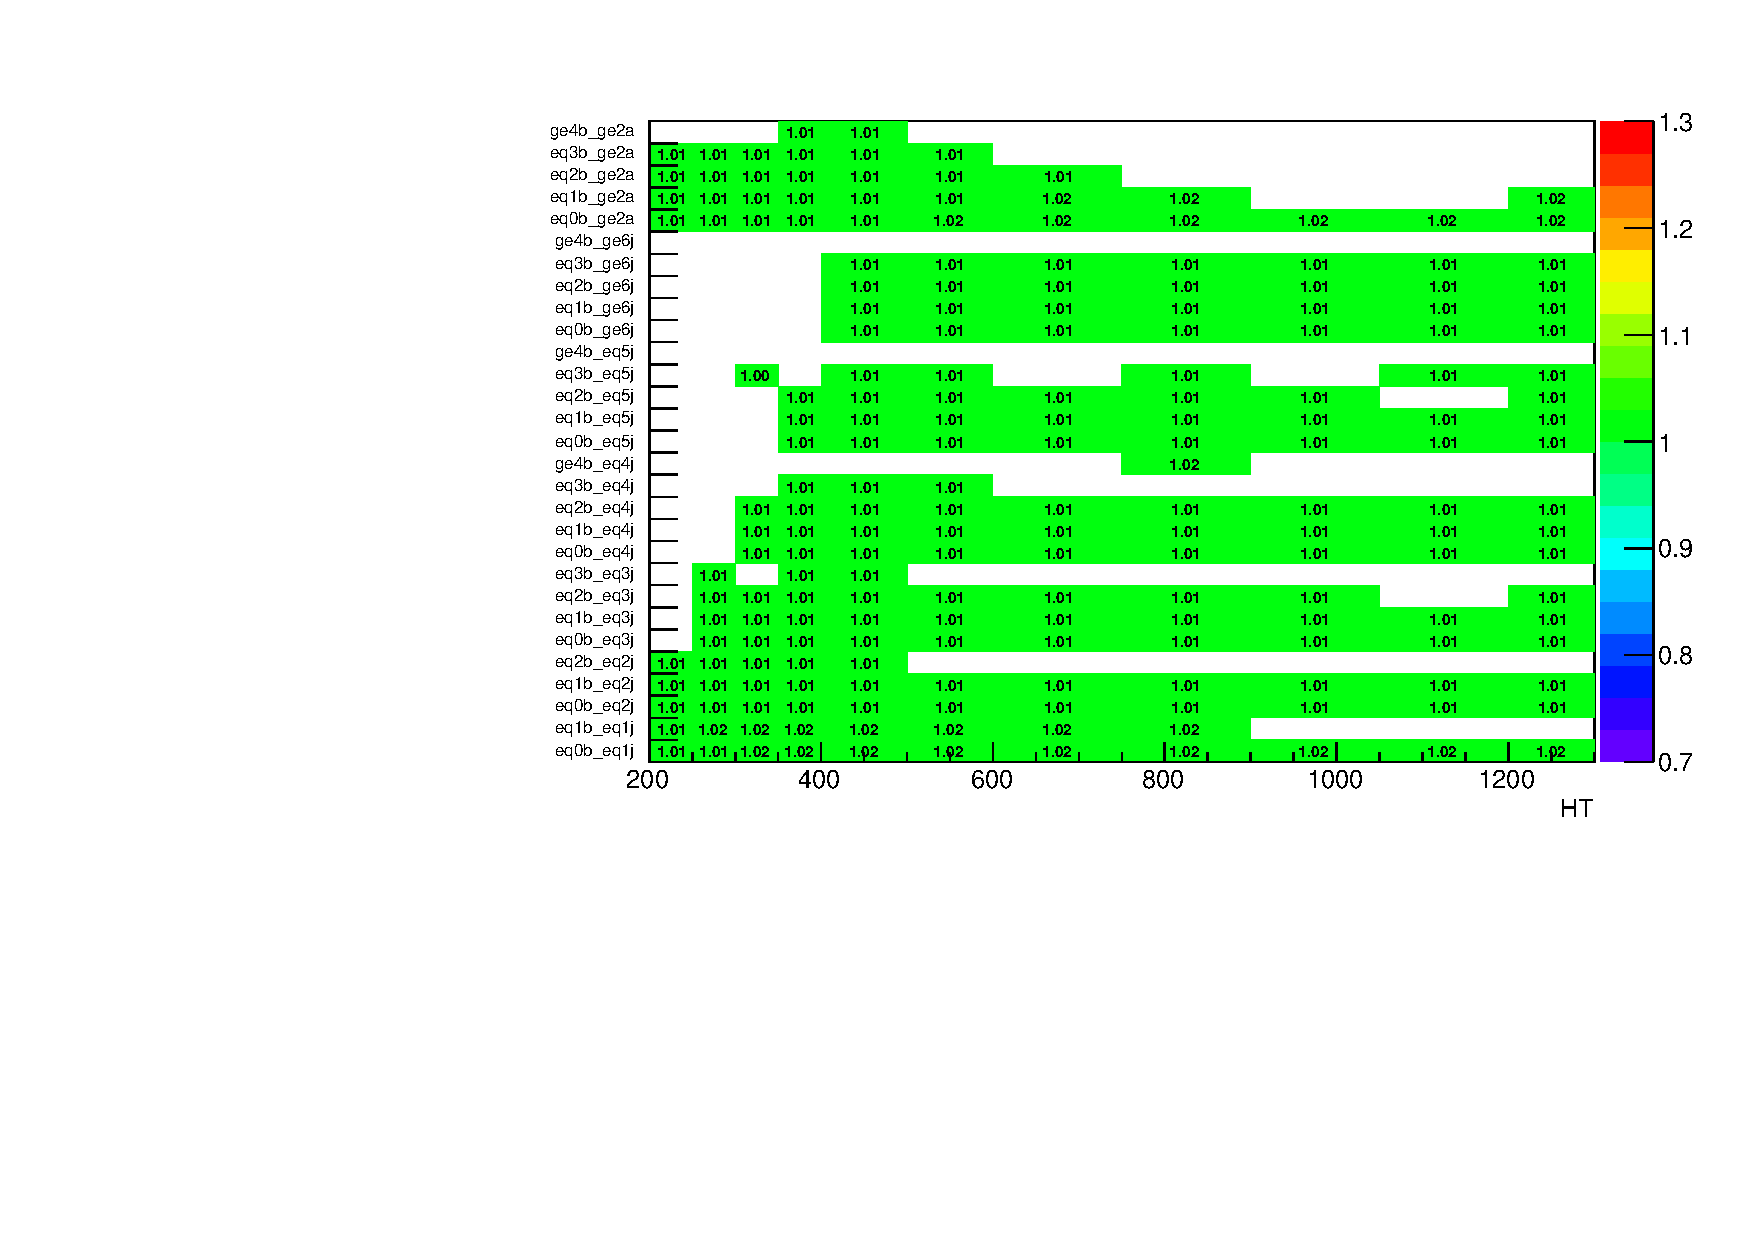
\includegraphics[width=0.5\textwidth]{figures/mcSystematics36p4fb/Ttw/mu/ratiotfh_ht_mht_allmuonSfWeight_Down.pdf}
  }\\

  \caption{\label{fig:tfSyst_muon_scale_factor_muToTtw} The relative change in the $\mj \rightarrow \mathrm{tt+W}$ transfer
  factors when varying muon scale factor in MC within its uncertainties, as a function of \scalht and jet category. 
  Variations corresponding to $+1\sigma$ ($-1\sigma$) are shown in the left (right) figure. 
  }
\end{figure}

\subsection{Jet energy scale}

\begin{figure}[!h]
  \centering
  \subfigure[JEC up variation]{
    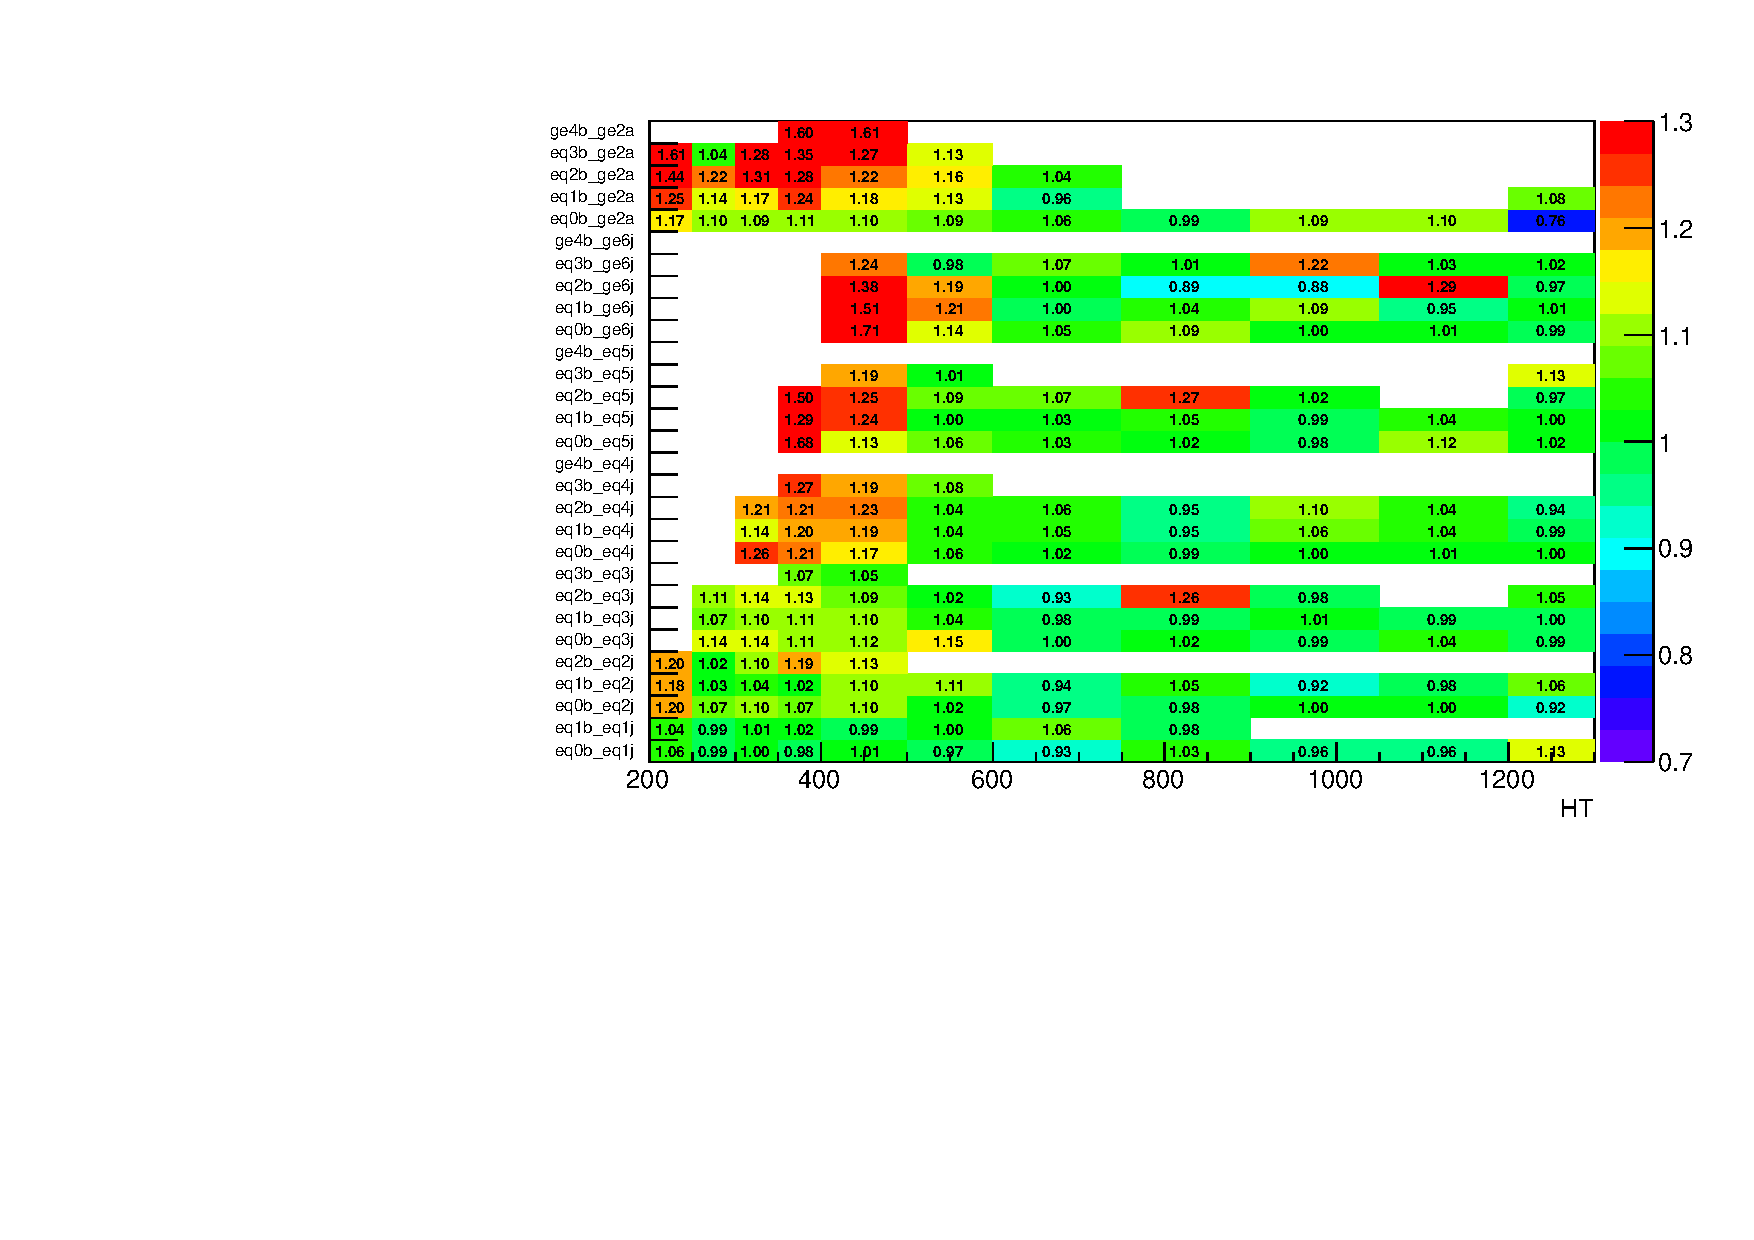
\includegraphics[width=0.5\textwidth]{figures/mcSystematics36p4fb/Ttw/mu/ratiotfh_ht_mht_alljecWeight_Up.pdf}
  } ~~
  \subfigure[JEC down variation]{
    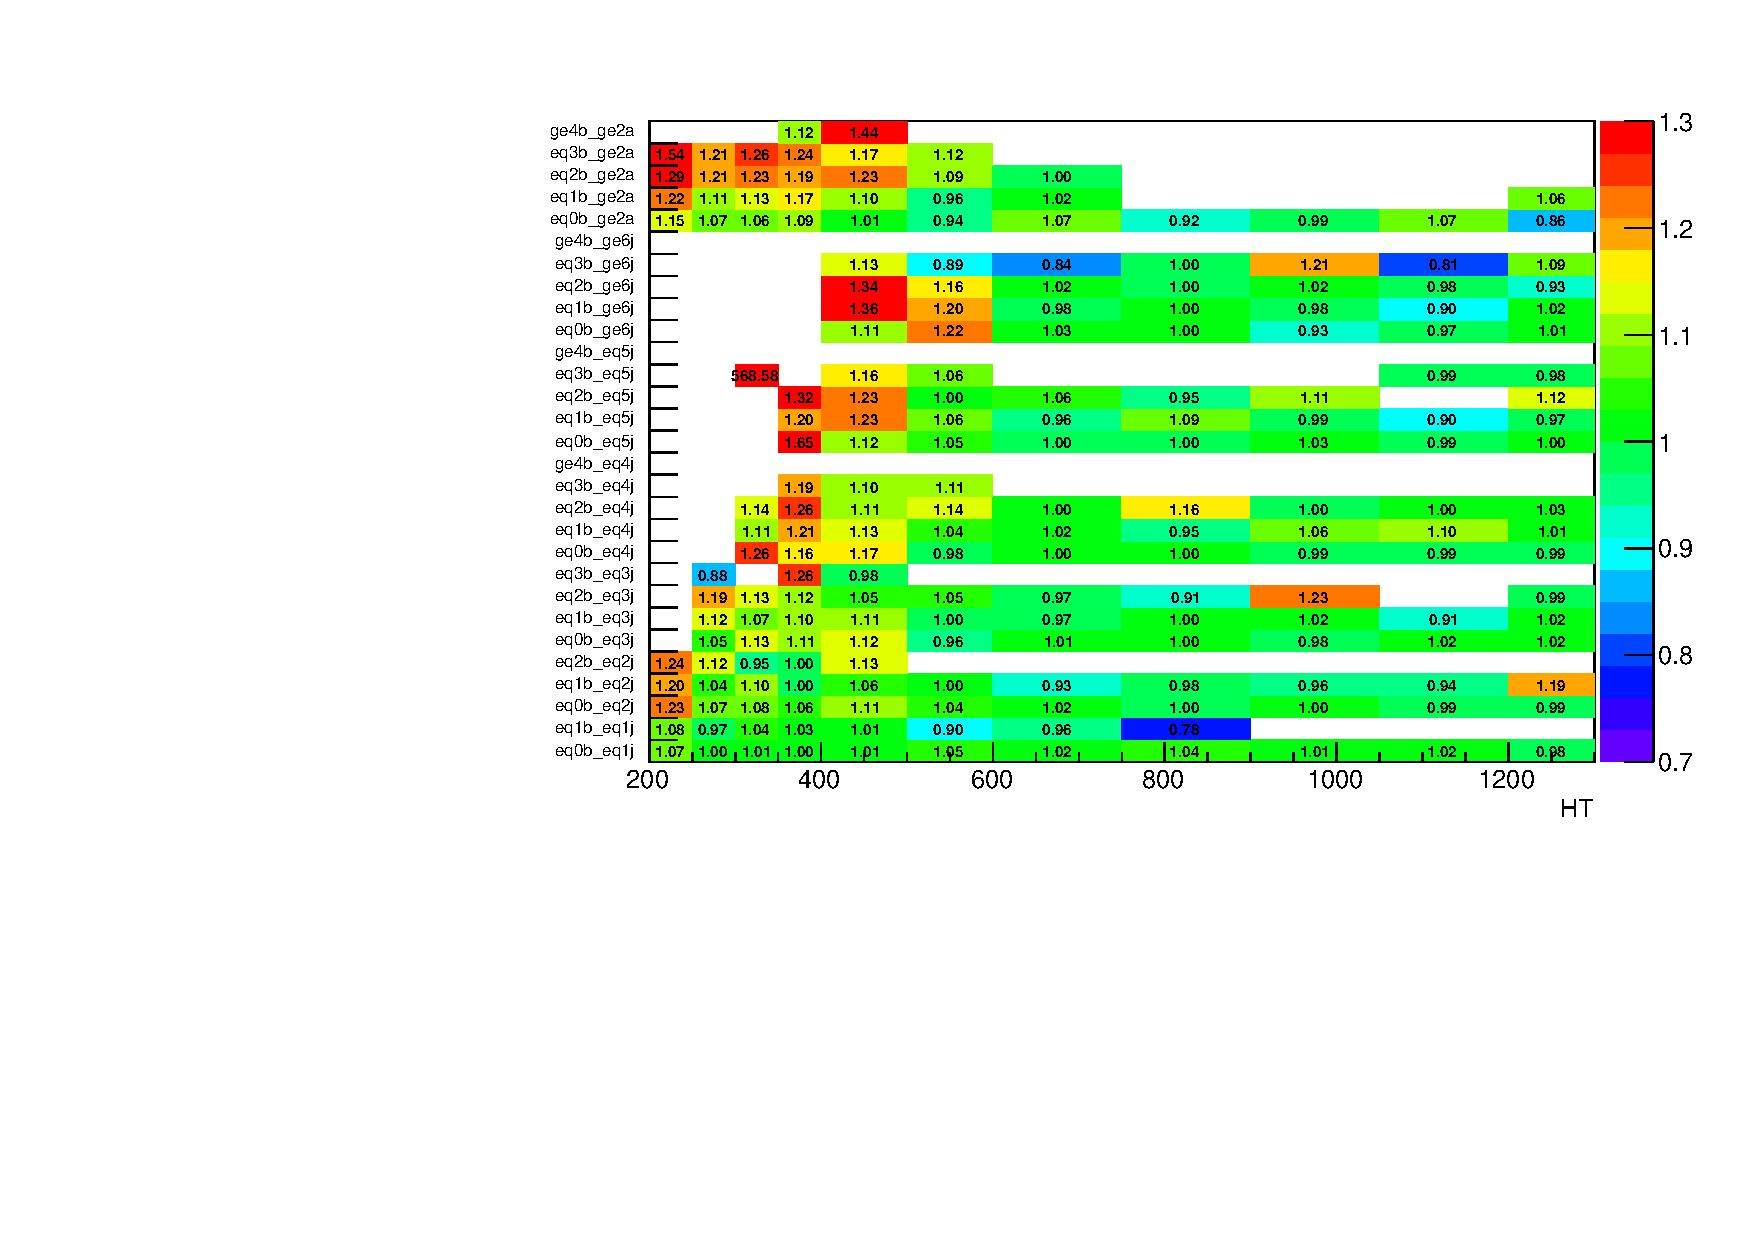
\includegraphics[width=0.5\textwidth]{figures/mcSystematics36p4fb/Ttw/mu/ratiotfh_ht_mht_alljecWeight_Down.pdf}
  }\\

  \caption{\label{fig:tfSyst_jec_muToTtw} The relative change in the
  $\mj \rightarrow \mathrm{\ttbar+W}$ transfer
  factors when varying JEC in MC within its uncertainties, as a function of \scalht and jet category. 
  Variations corresponding to $+1\sigma$ ($-1\sigma$) are shown in the left (right) figure. 
  }
\end{figure}

\clearpage
\subsection{b-tagging efficiency}

\begin{figure}[!h]
  \centering
  \subfigure[b-tag SF (heavy) up variation]{
    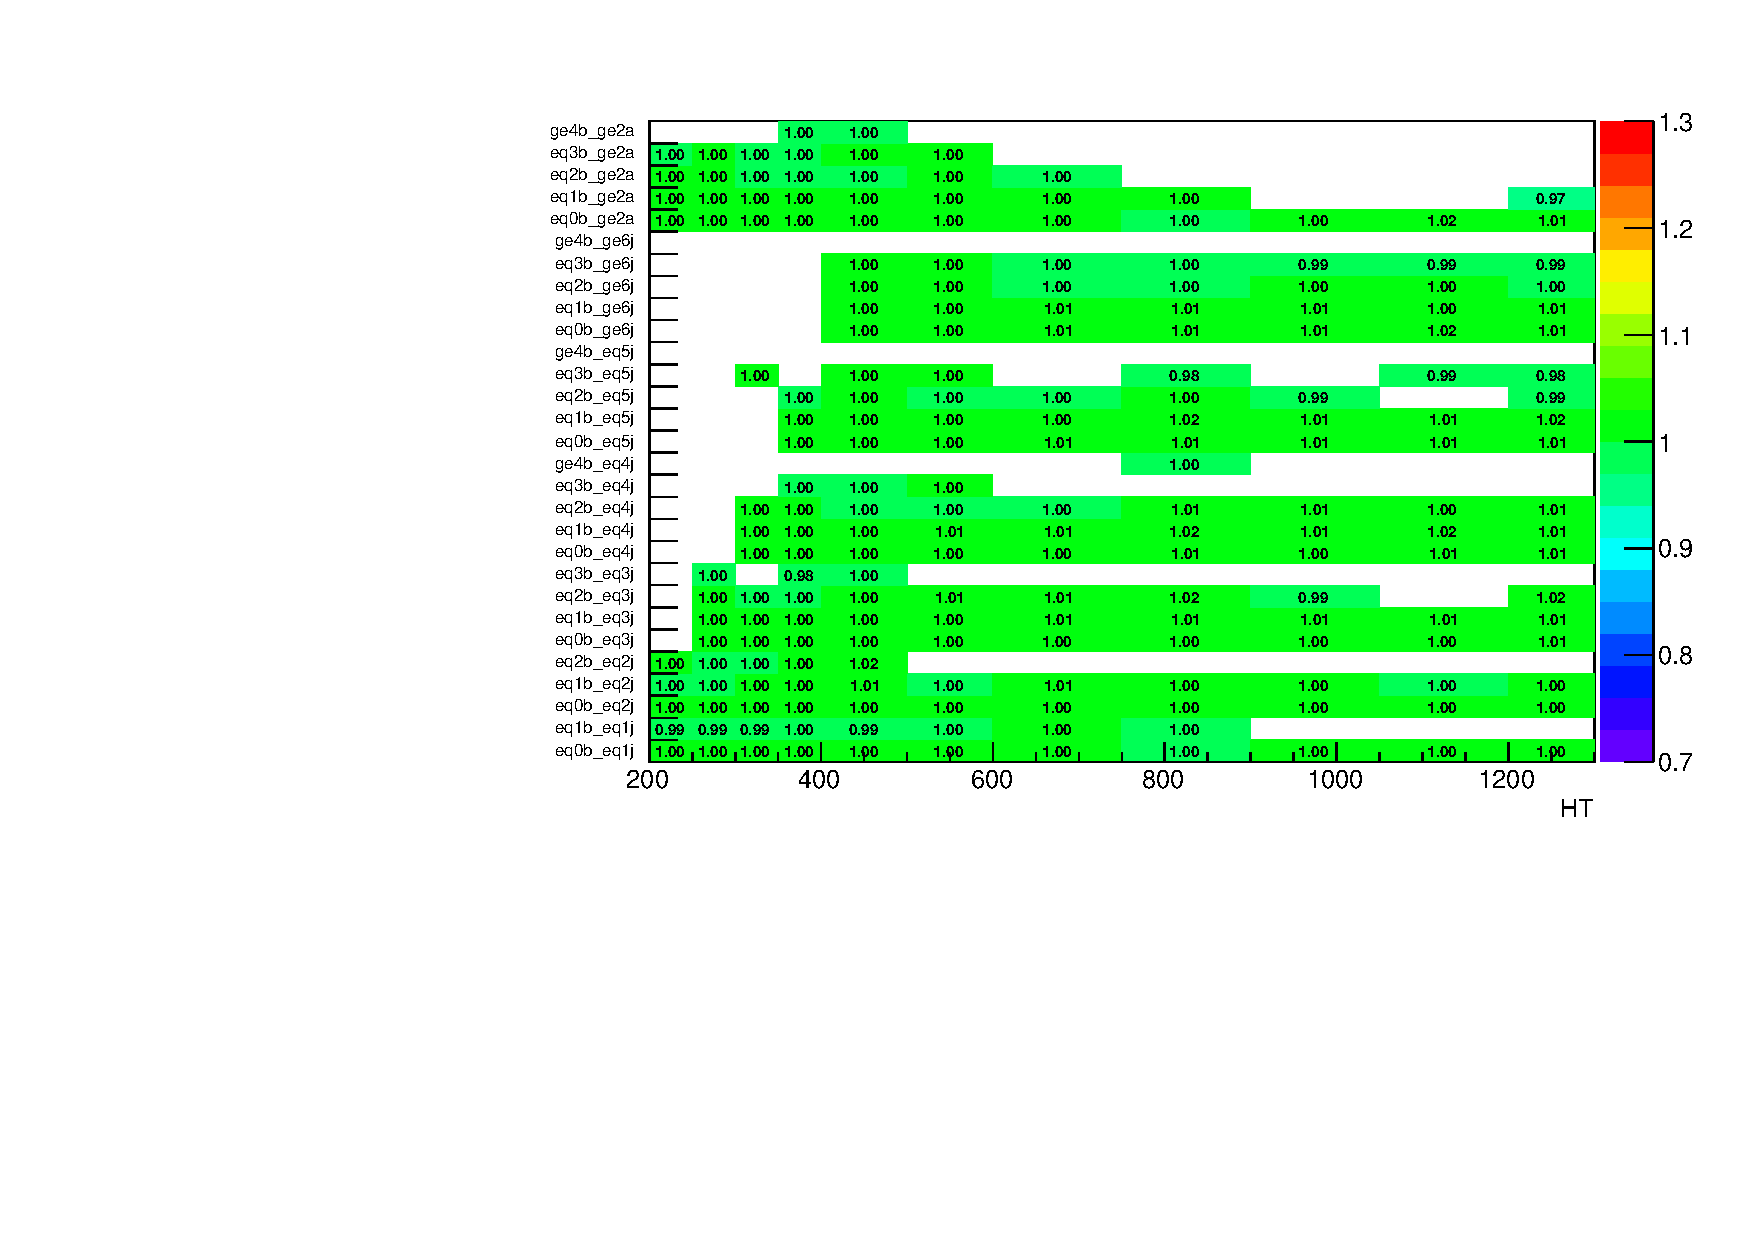
\includegraphics[width=0.5\textwidth]{figures/mcSystematics36p4fb/Ttw/mu/ratiotfh_ht_mht_allbsfWeight_Up.pdf}
  } ~~
  \subfigure[b-tag SF (heavy) down variation]{
    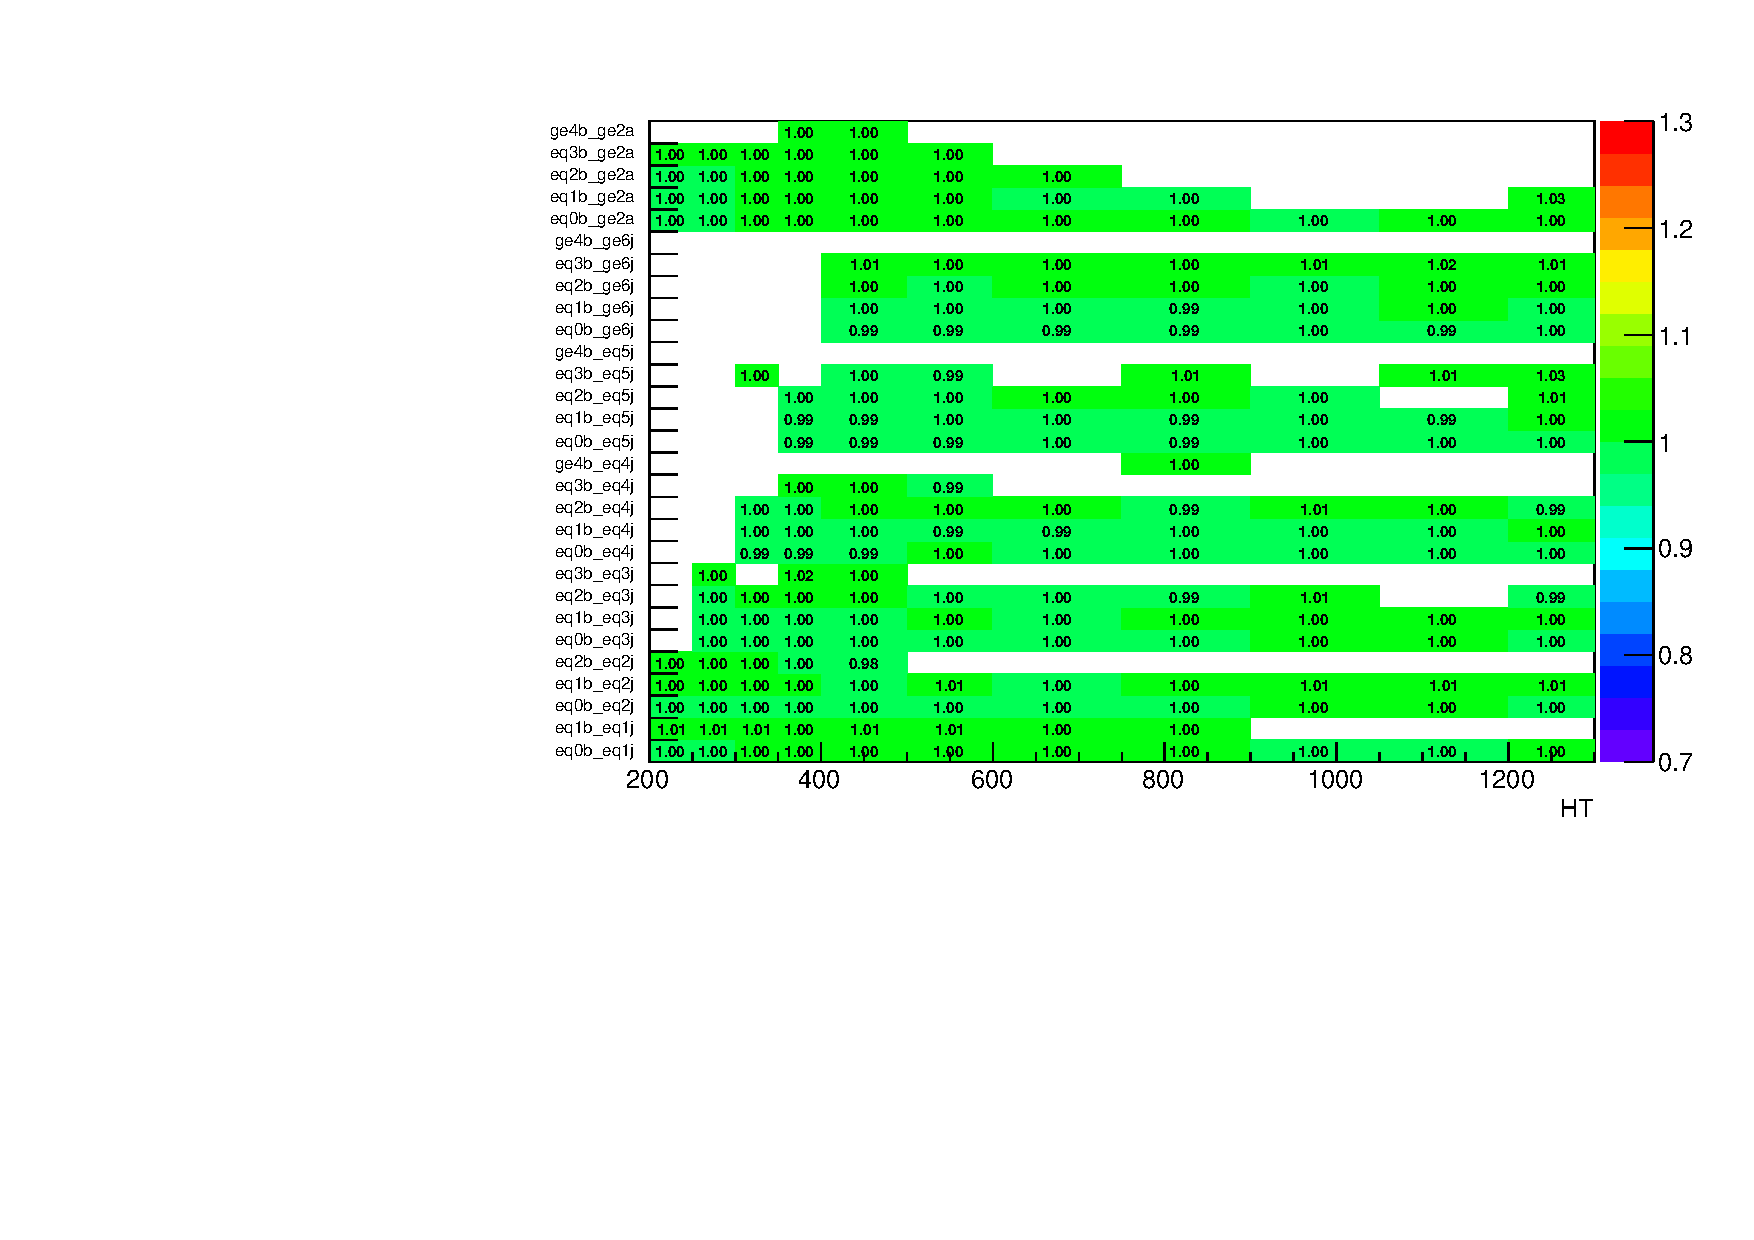
\includegraphics[width=0.5\textwidth]{figures/mcSystematics36p4fb/Ttw/mu/ratiotfh_ht_mht_allbsfWeight_Down.pdf}
  }\\

  \caption{\label{fig:tfSyst_bsf_muToTtw} The relative change in the $\mj \rightarrow \mathrm{tt+W}$ transfer
  factors when varying b-tag SF for heavy jets in MC within its uncertainties, as a function of \scalht and jet category. 
  Variations corresponding to $+1\sigma$ ($-1\sigma$) are shown in the left (right) figure. 
  }
\end{figure}

\subsection{b-tagging mistag}

\begin{figure}[!h]
  \centering
  \subfigure[b-tag SF (light) up variation]{
    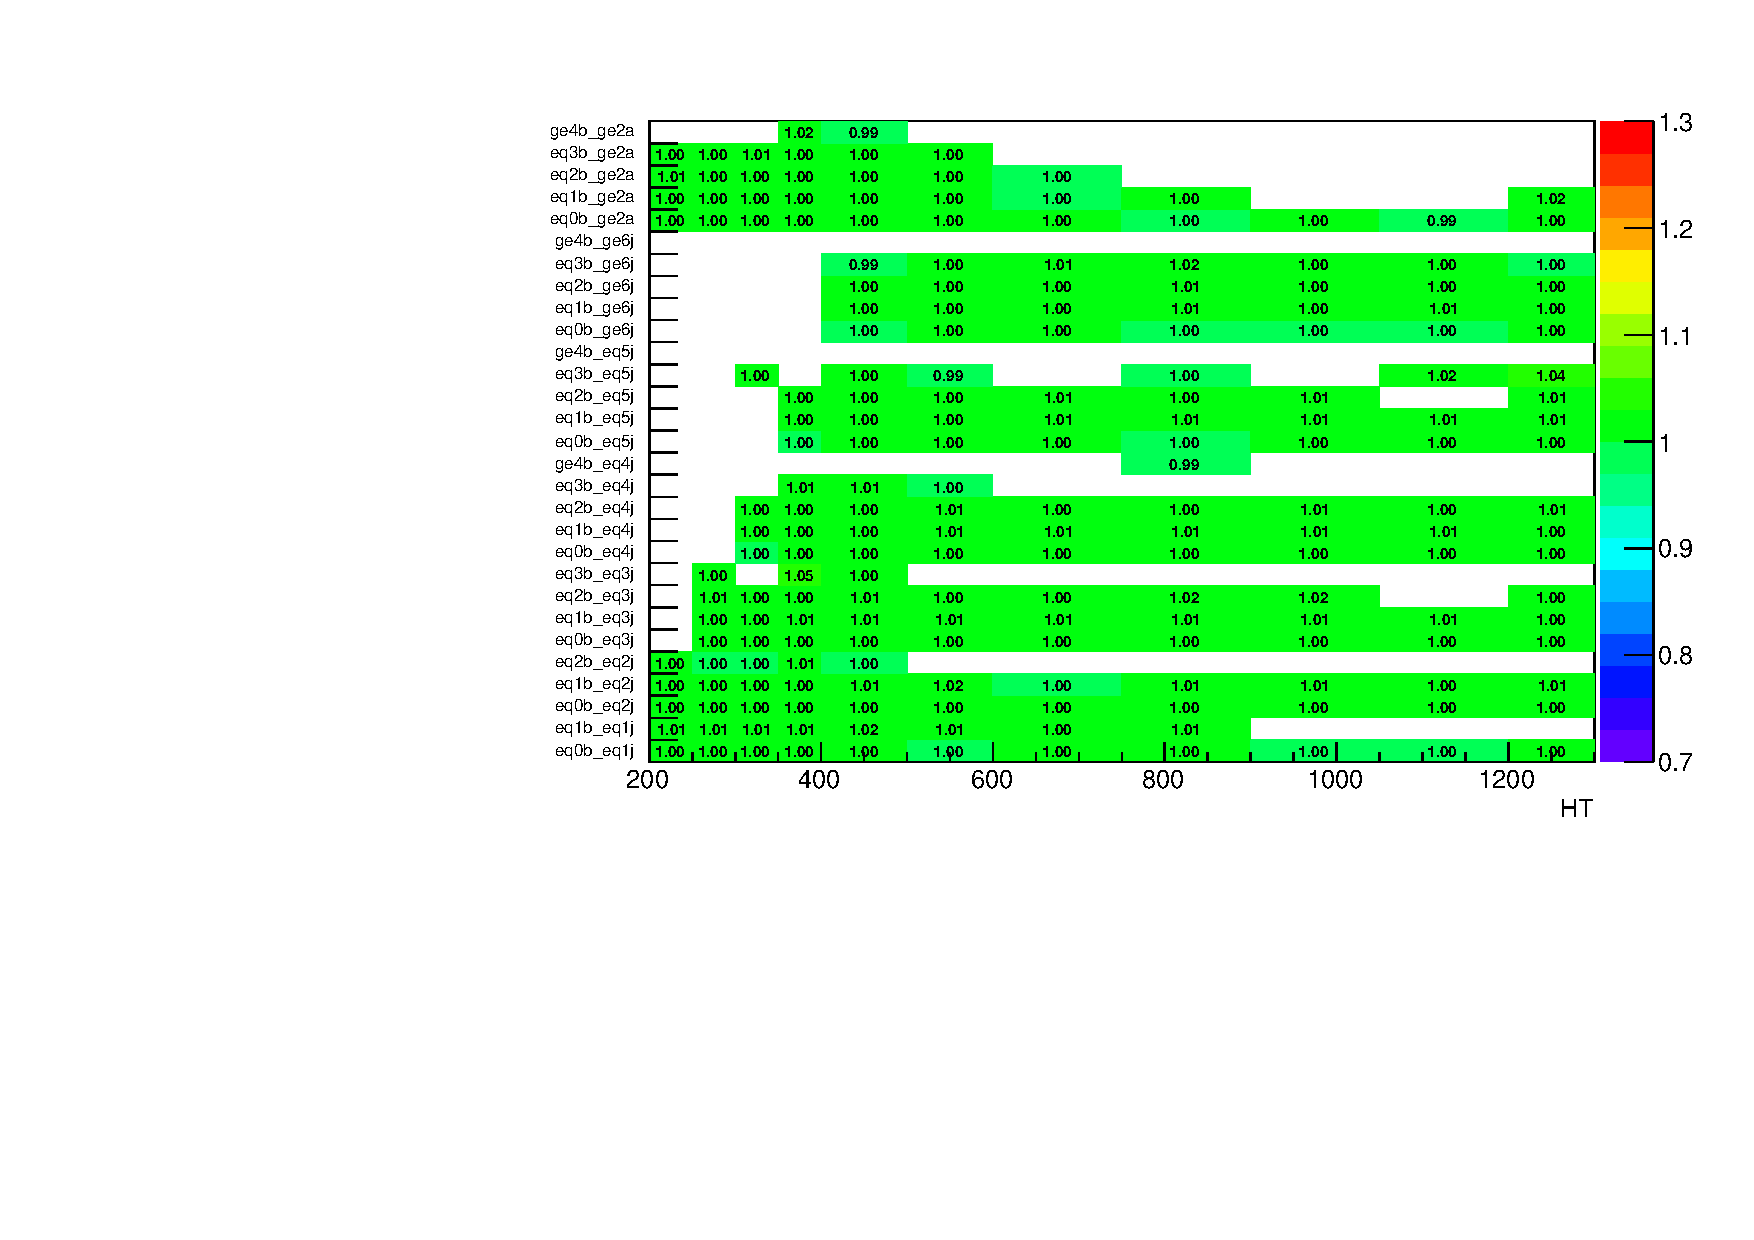
\includegraphics[width=0.5\textwidth]{figures/mcSystematics36p4fb/Ttw/mu/ratiotfh_ht_mht_allbsfLightWeight_Up.pdf}
  } ~~
  \subfigure[b-tag SF (light) down variation]{
    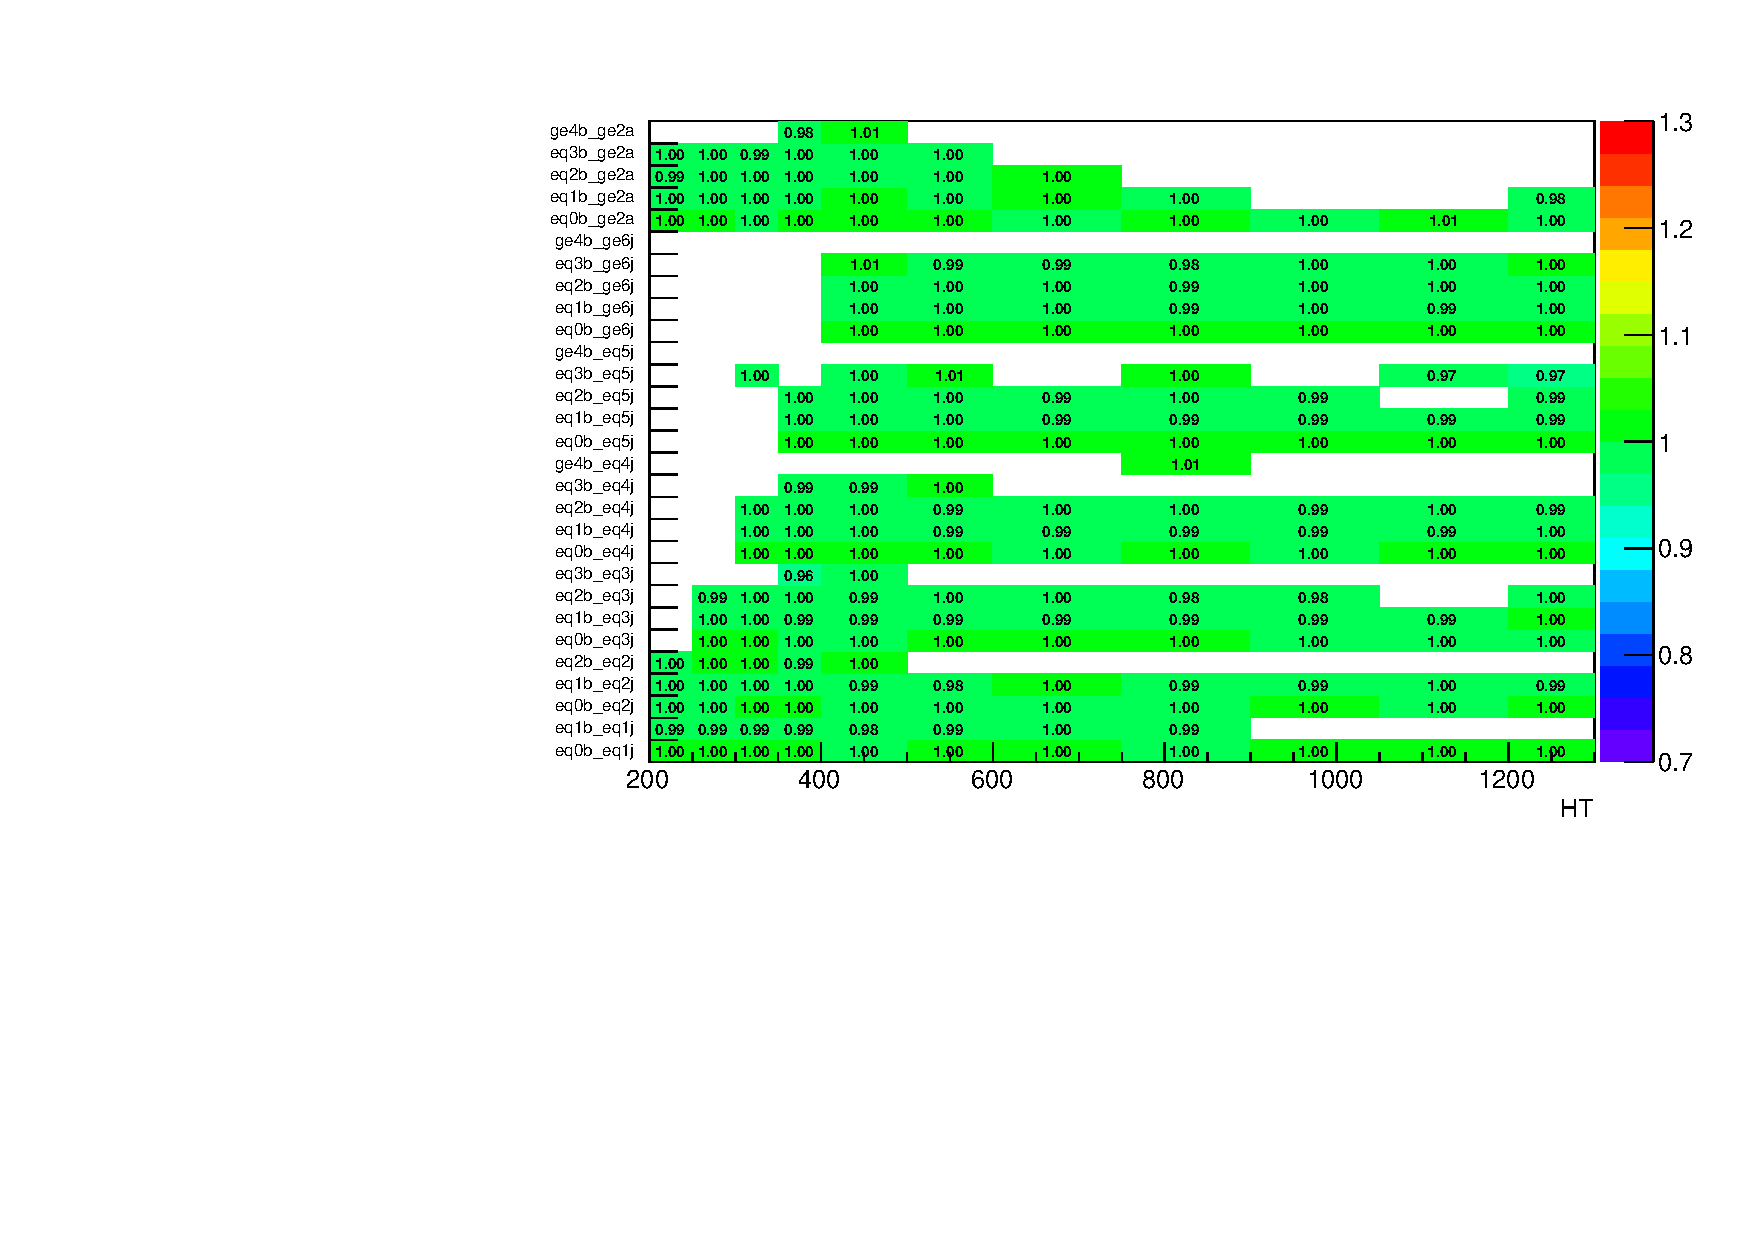
\includegraphics[width=0.5\textwidth]{figures/mcSystematics36p4fb/Ttw/mu/ratiotfh_ht_mht_allbsfLightWeight_Down.pdf}
  }\\

  \caption{\label{fig:tfSyst_bsfl_muToTtw} The relative change in the $\mj \rightarrow \mathrm{tt+W}$ transfer
  factors when varying b-tag SF for light jets in MC within its uncertainties, as a function of \scalht and jet category. 
  Variations corresponding to $+1\sigma$ ($-1\sigma$) are shown in the left (right) figure. 
  }
\end{figure}

\clearpage
\subsection{Extrapolation in \texorpdfstring{\alphat}{AlphaT}}

\begin{figure}[h!]
  \begin{center}
    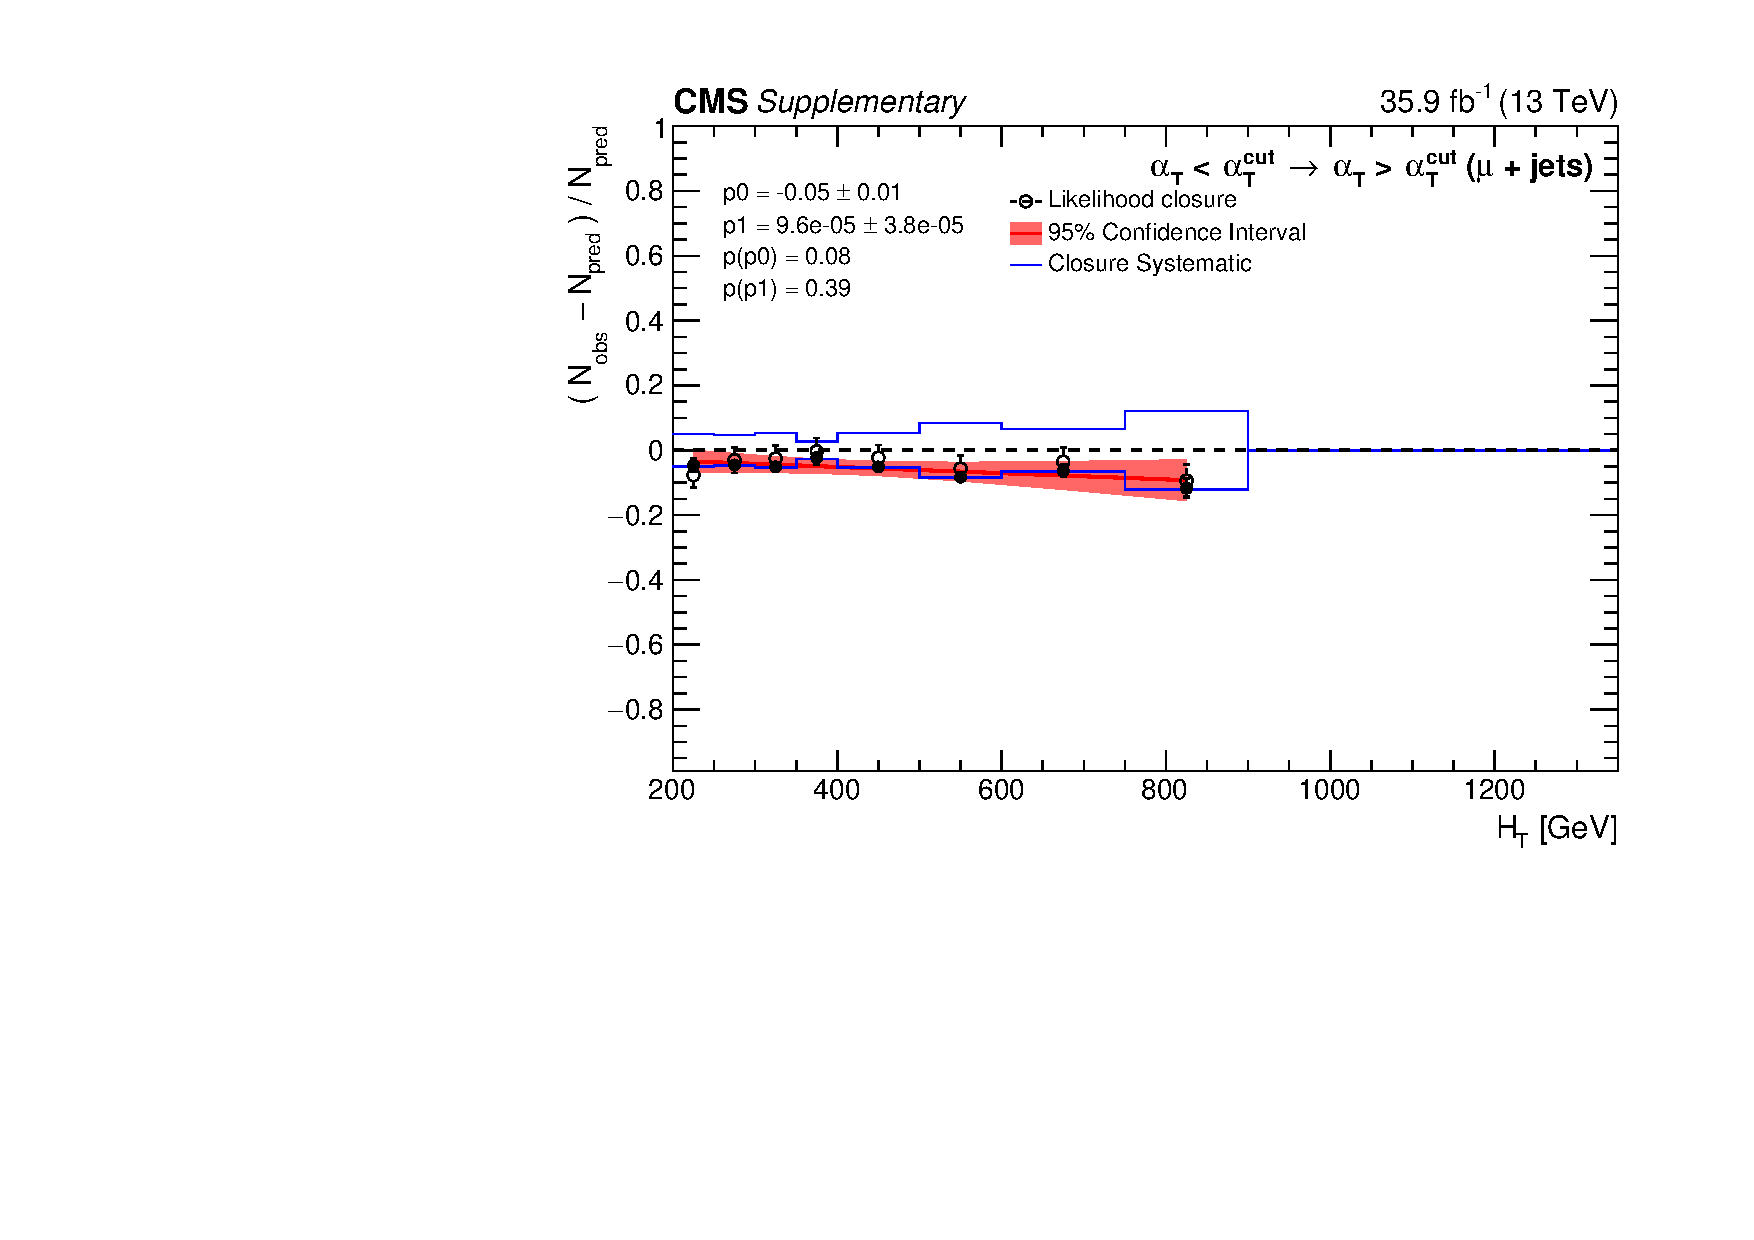
\includegraphics[width=0.45\textwidth]{figures/closureTests/AlphaT/SingleMu_alphaTExtrapolation_ht.pdf}~
    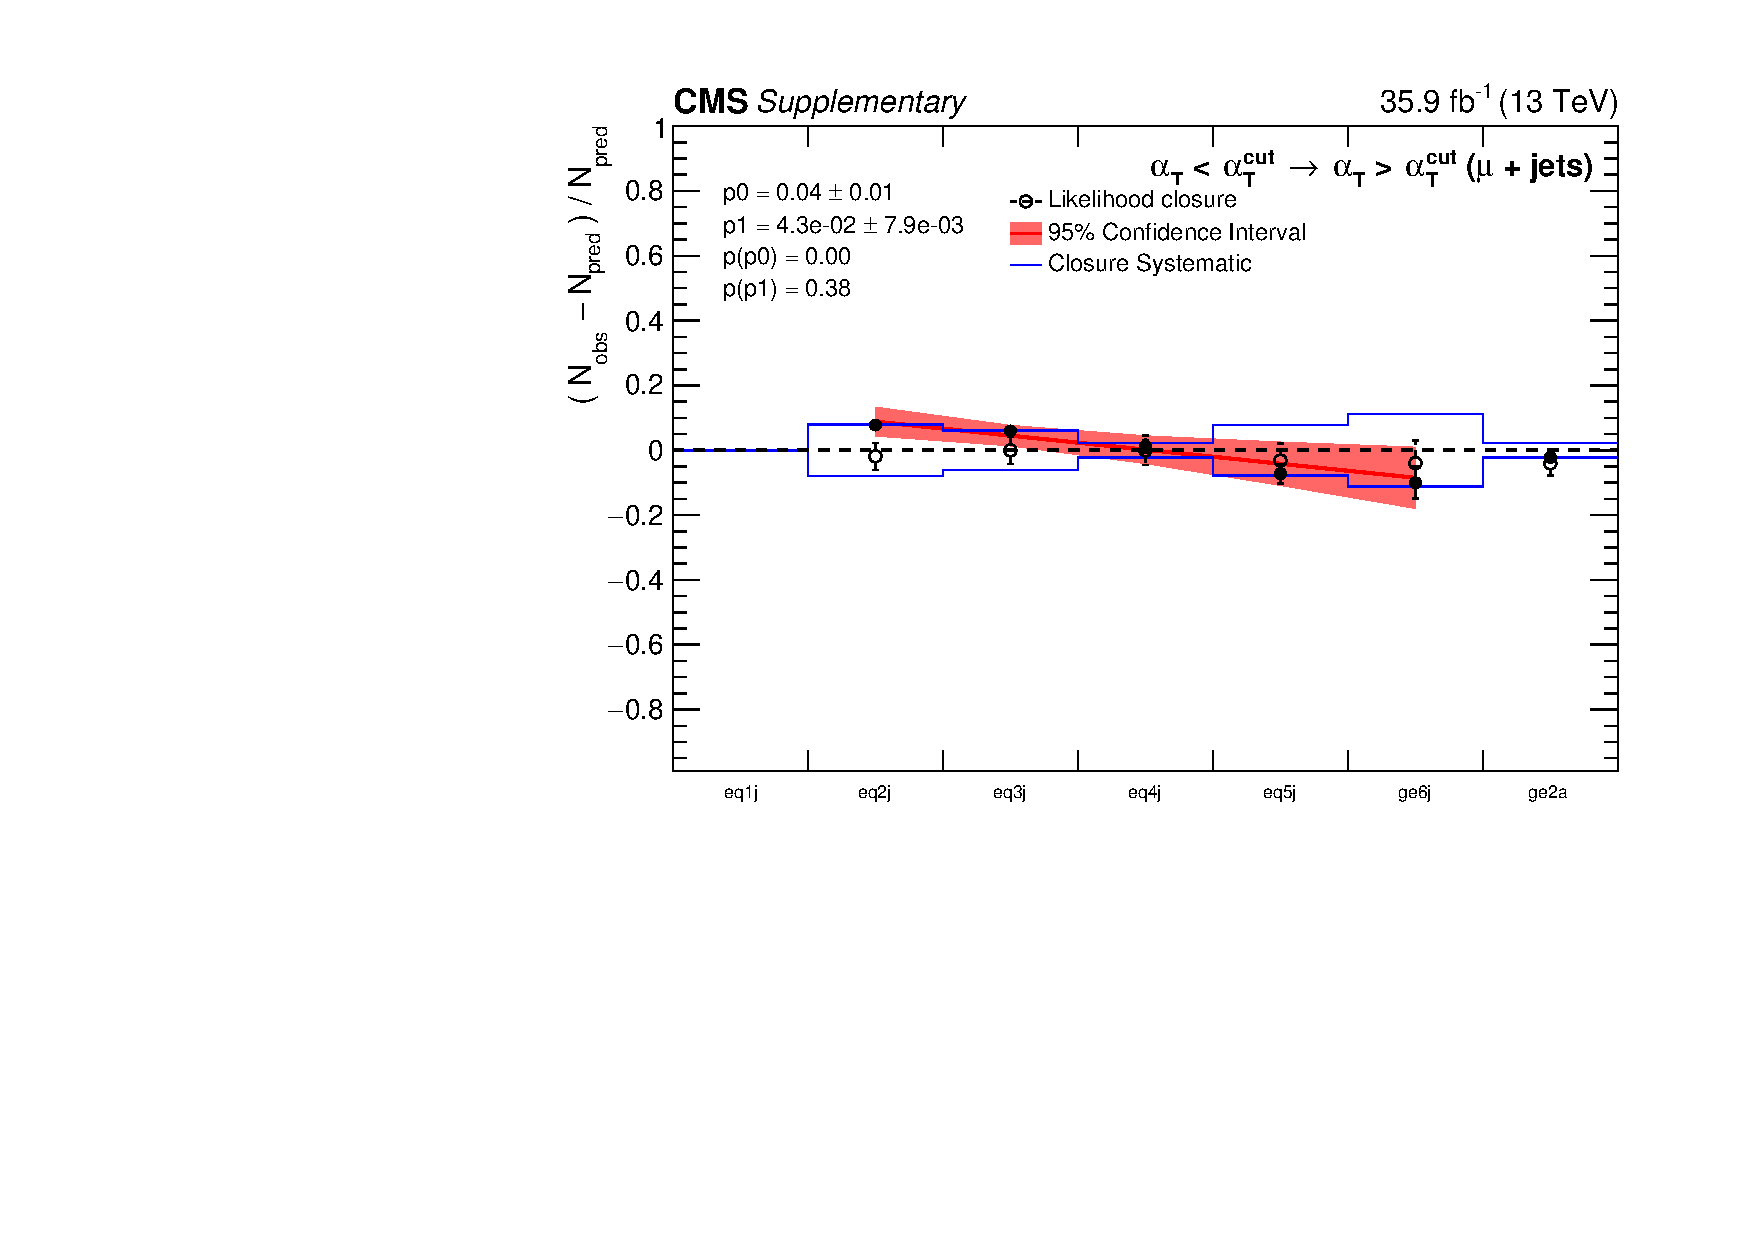
\includegraphics[width=0.45\textwidth]{figures/closureTests/AlphaT/SingleMu_alphaTExtrapolation_nJet.pdf}\\
    \caption{Data-driven closure tests probing the modelling of an
      extrapolation in the \alphat variable with the \mj sample. The
      level of closure (solid markers) is indicated as a function of
      \scalht (left) and \njet (right). The blue histogram indicates
      the quadrature sum of the magnitude of non-closure and its
      statistical uncertainty. The post-fit closure (open markers) is
      also shown (see text for details).  }
    \label{fig:closure_AlphaT_mu}
  \end{center} 
\end{figure}

\begin{figure}[h!]
  \begin{center}
    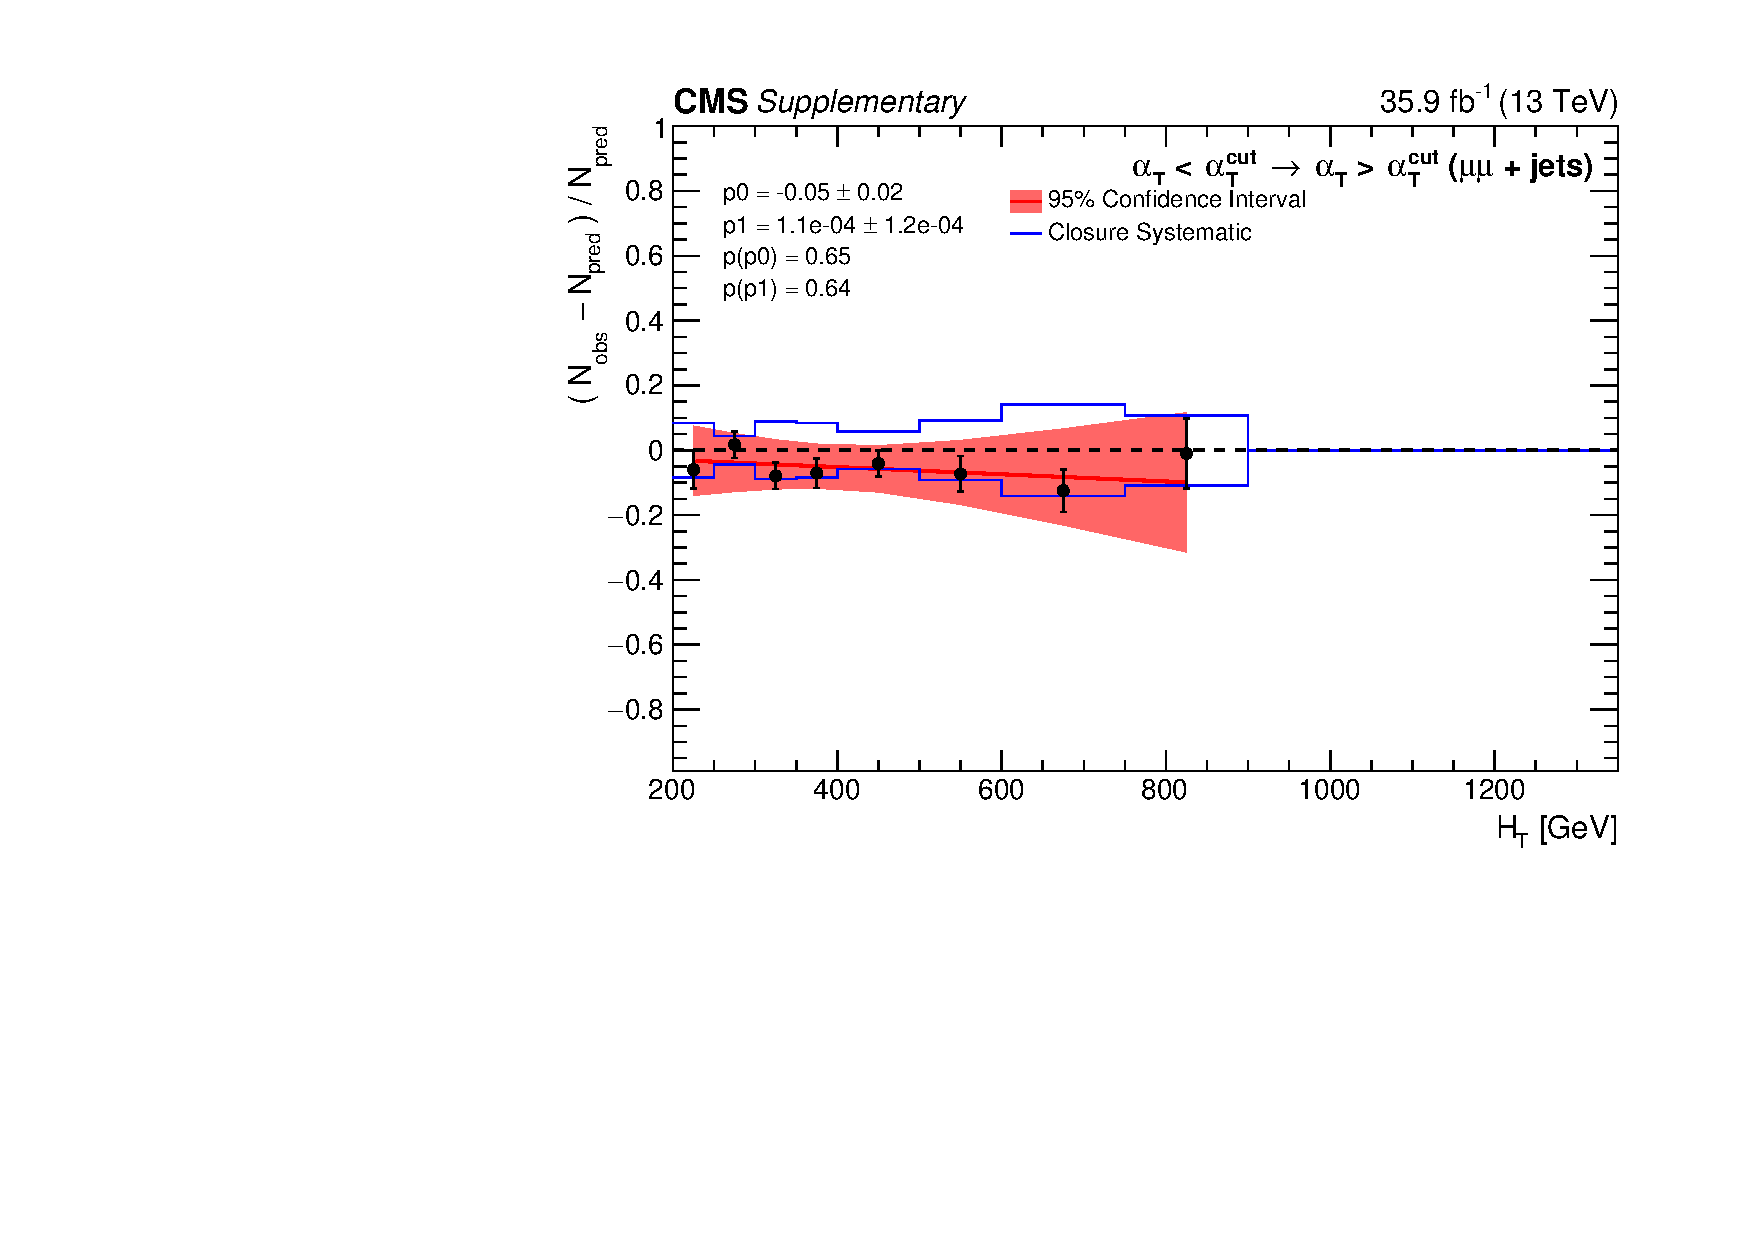
\includegraphics[width=0.45\textwidth]{figures/closureTests/AlphaT/DoubleMu_alphaTExtrapolation_ht.pdf}~
    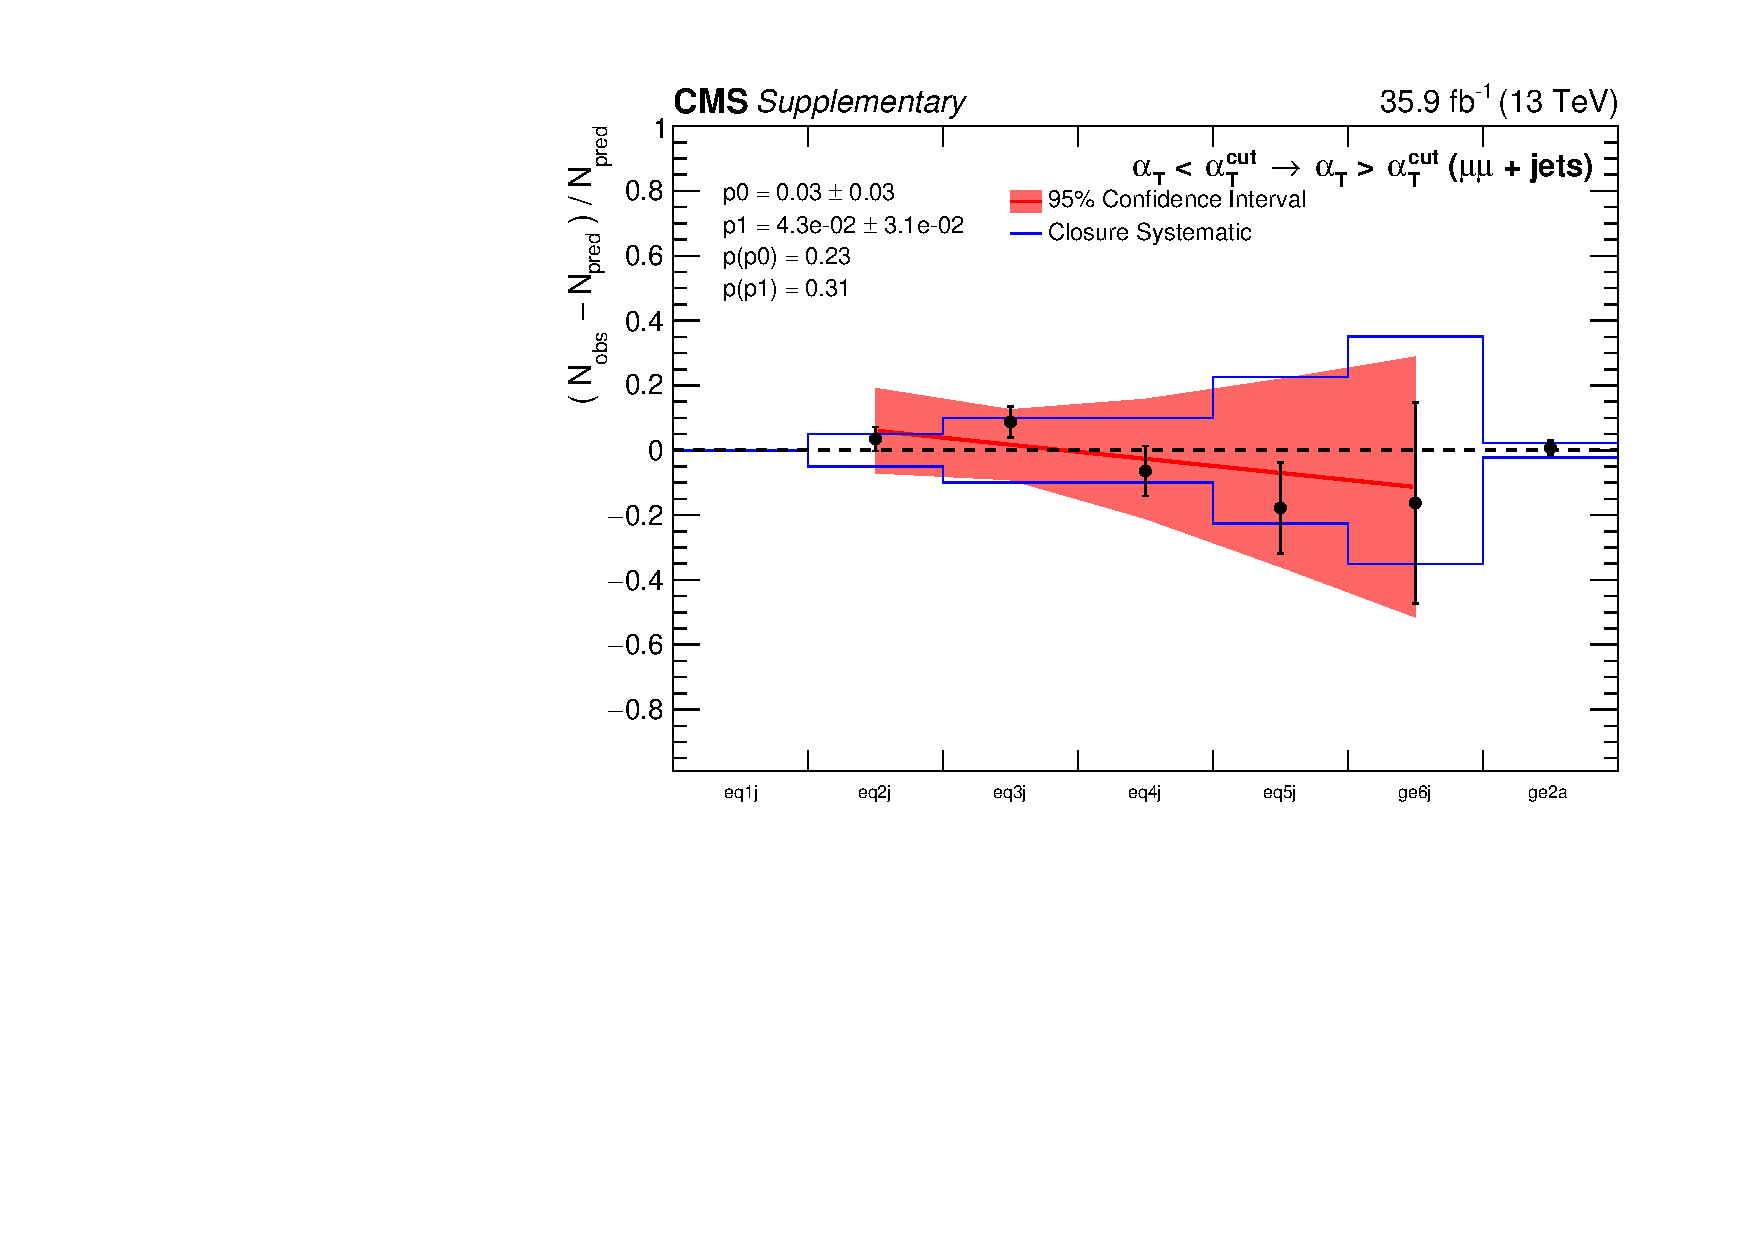
\includegraphics[width=0.45\textwidth]{figures/closureTests/AlphaT/DoubleMu_alphaTExtrapolation_nJet.pdf}\\ 
    \caption{As for Fig.~\ref{fig:closure_AlphaT_mu} but probing the
      modelling of an extrapolation in the \alphat variable with the
      \mmj sample.
    }
    \label{fig:closure_AlphaT_mumu}
  \end{center} 
\end{figure}

%\begin{figure}[h!]
%  \begin{center}
%    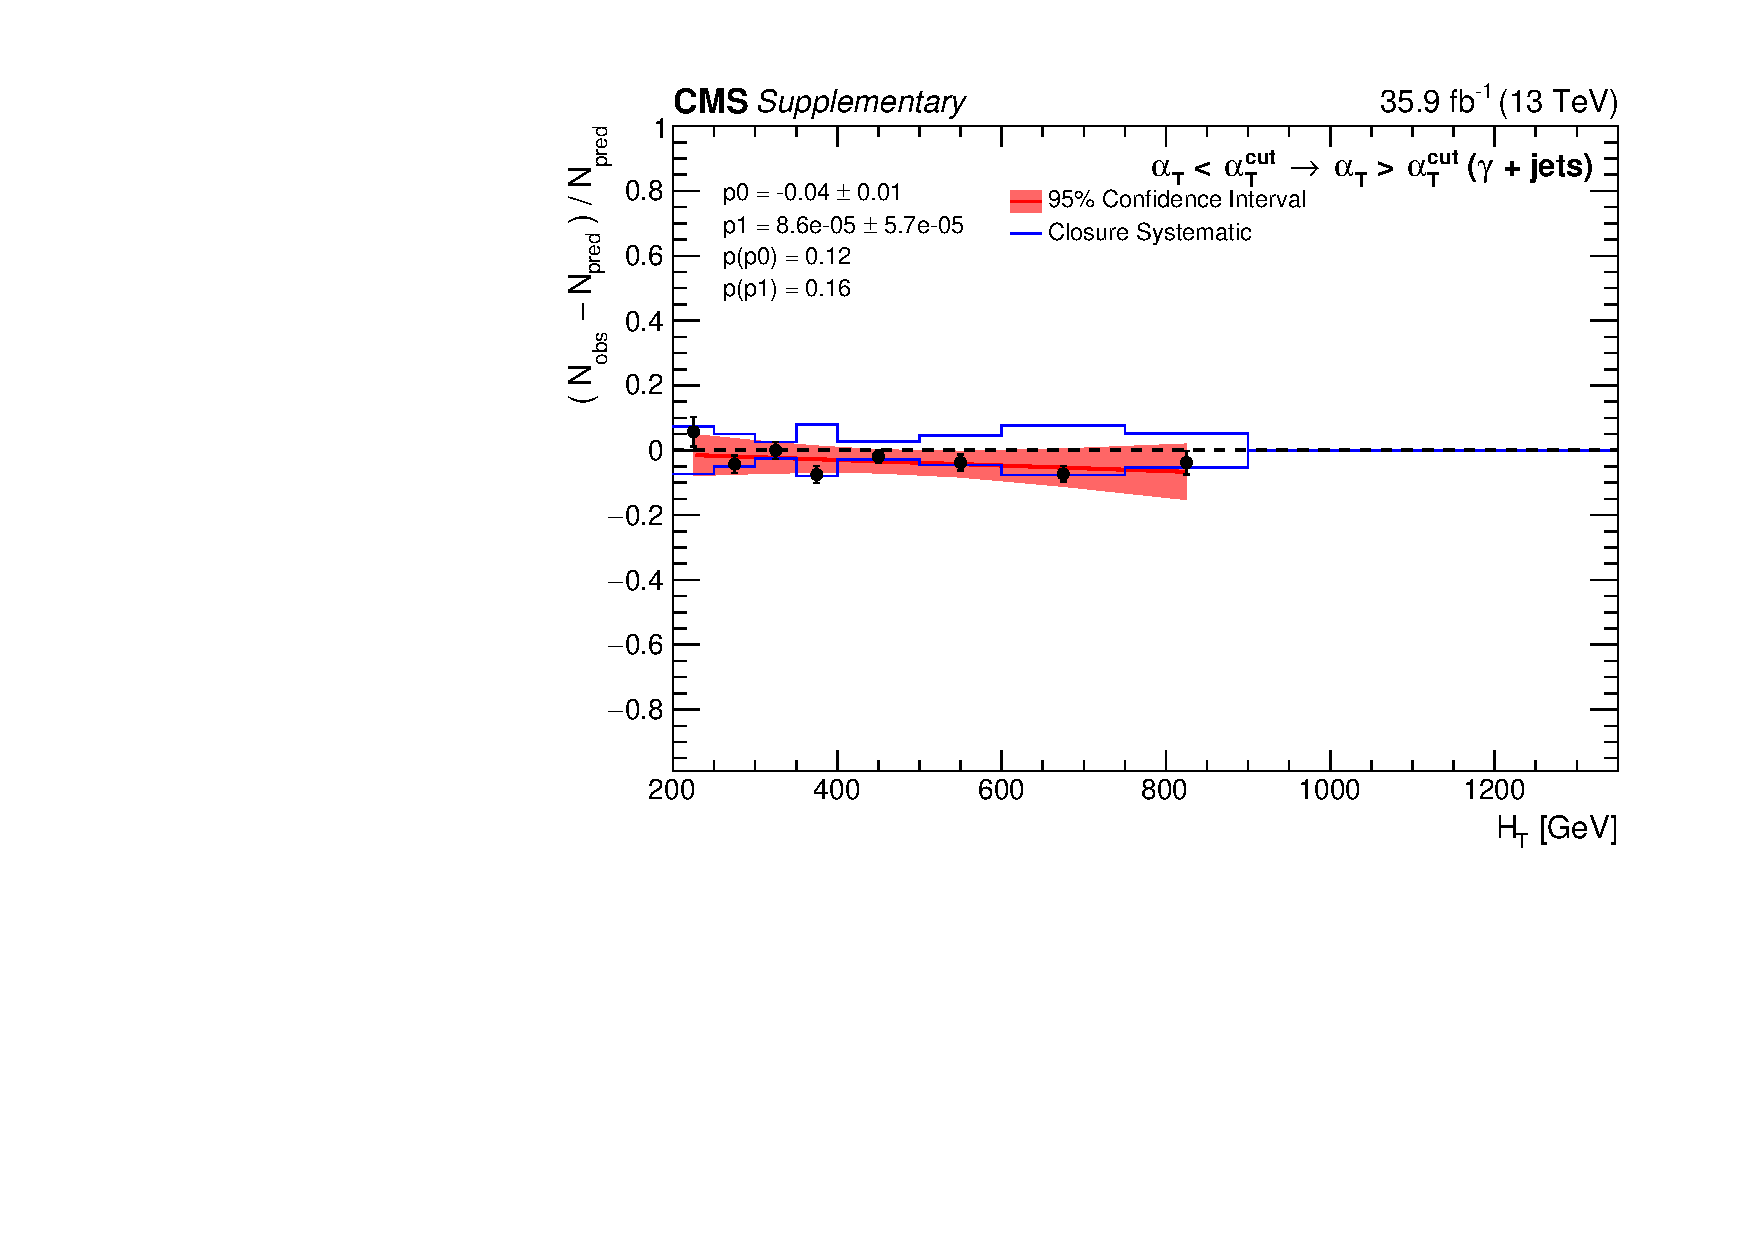
\includegraphics[width=0.45\textwidth]{figures/closureTests/AlphaT/SinglePhoton_alphaTExtrapolation_ht.pdf}~
%    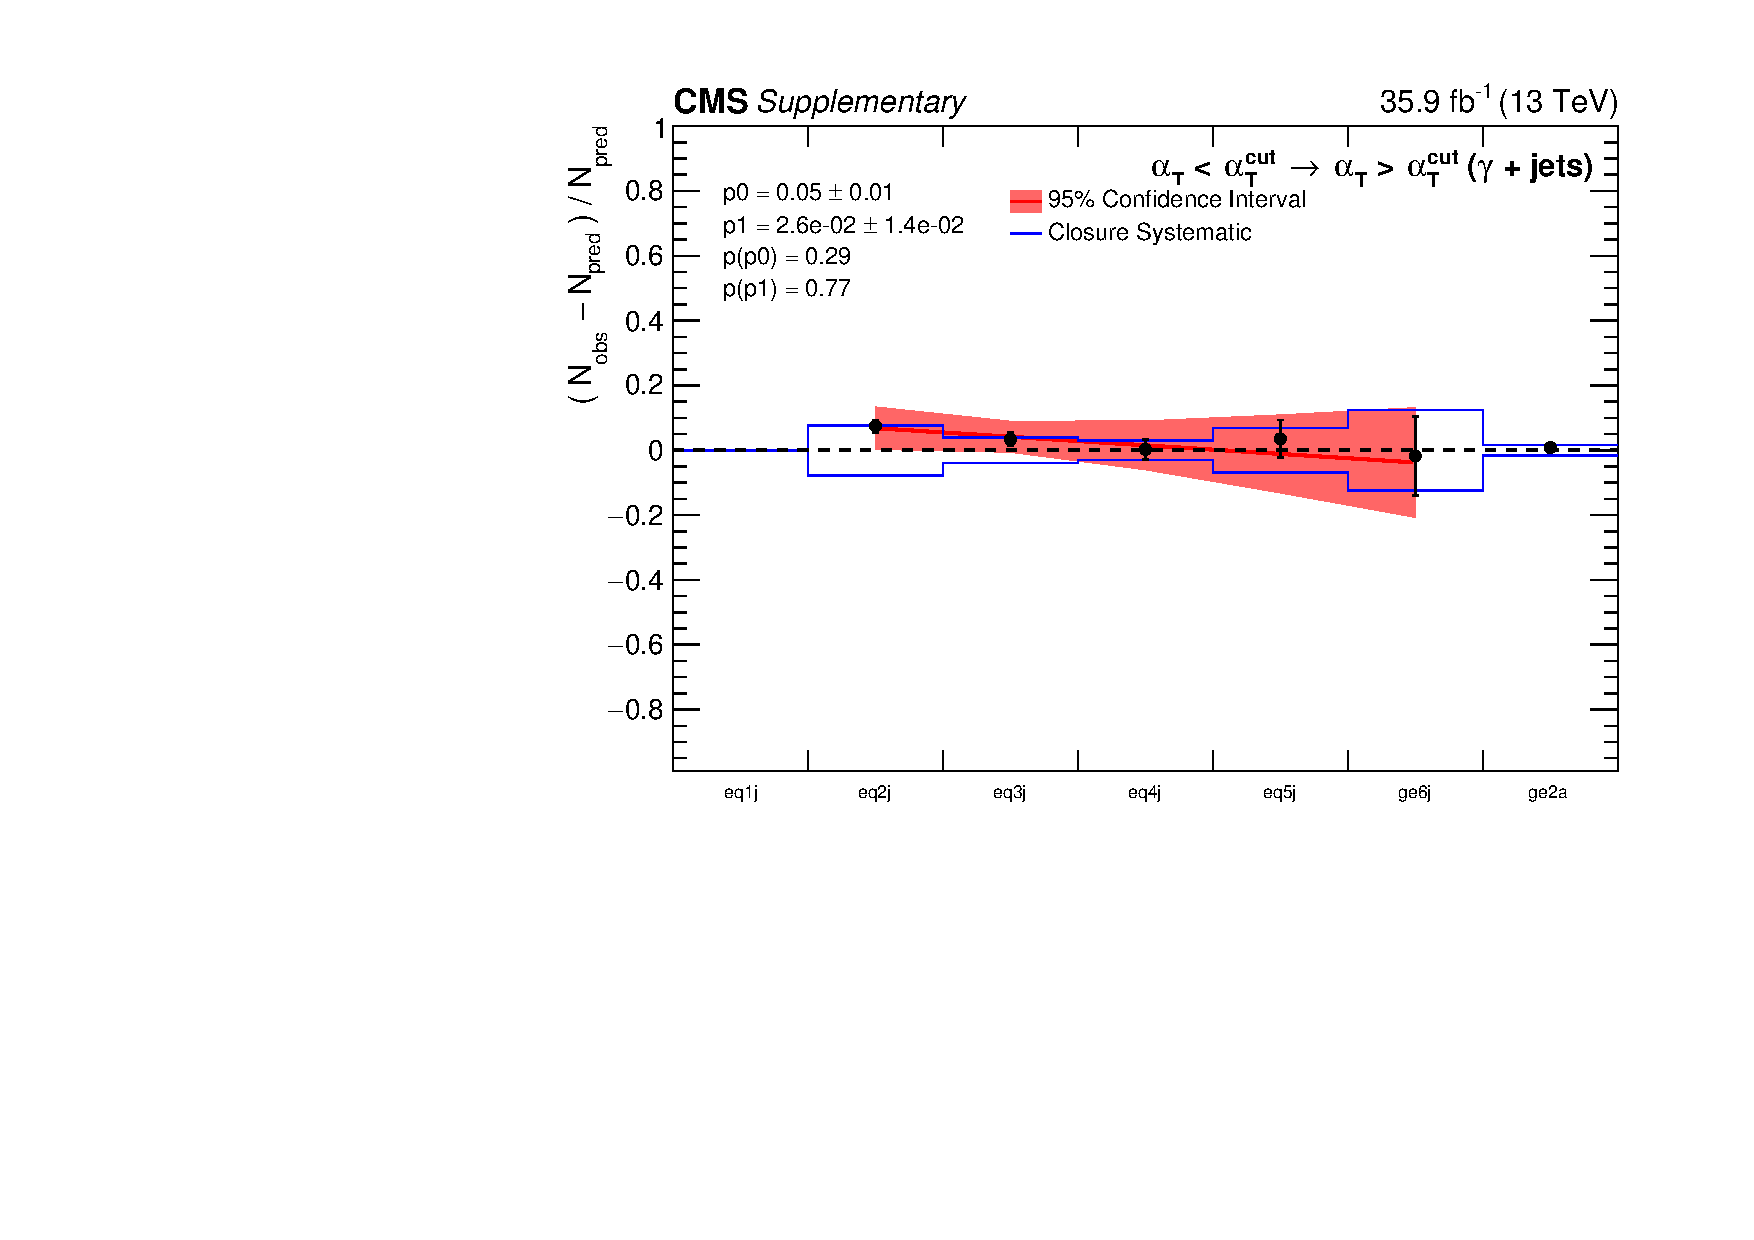
\includegraphics[width=0.45\textwidth]{figures/closureTests/AlphaT/SinglePhoton_alphaTExtrapolation_nJet.pdf}\\ 
%    \caption{As for Fig.~\ref{fig:closure_AlphaT_mu} but probing the
%      modelling of an extrapolation in the \alphat variable with the
%      \gj sample.
%    }
%    \label{fig:closure_AlphaT_phot}
%  \end{center} 
%\end{figure}

\begin{figure}[h!]
  \begin{center}
    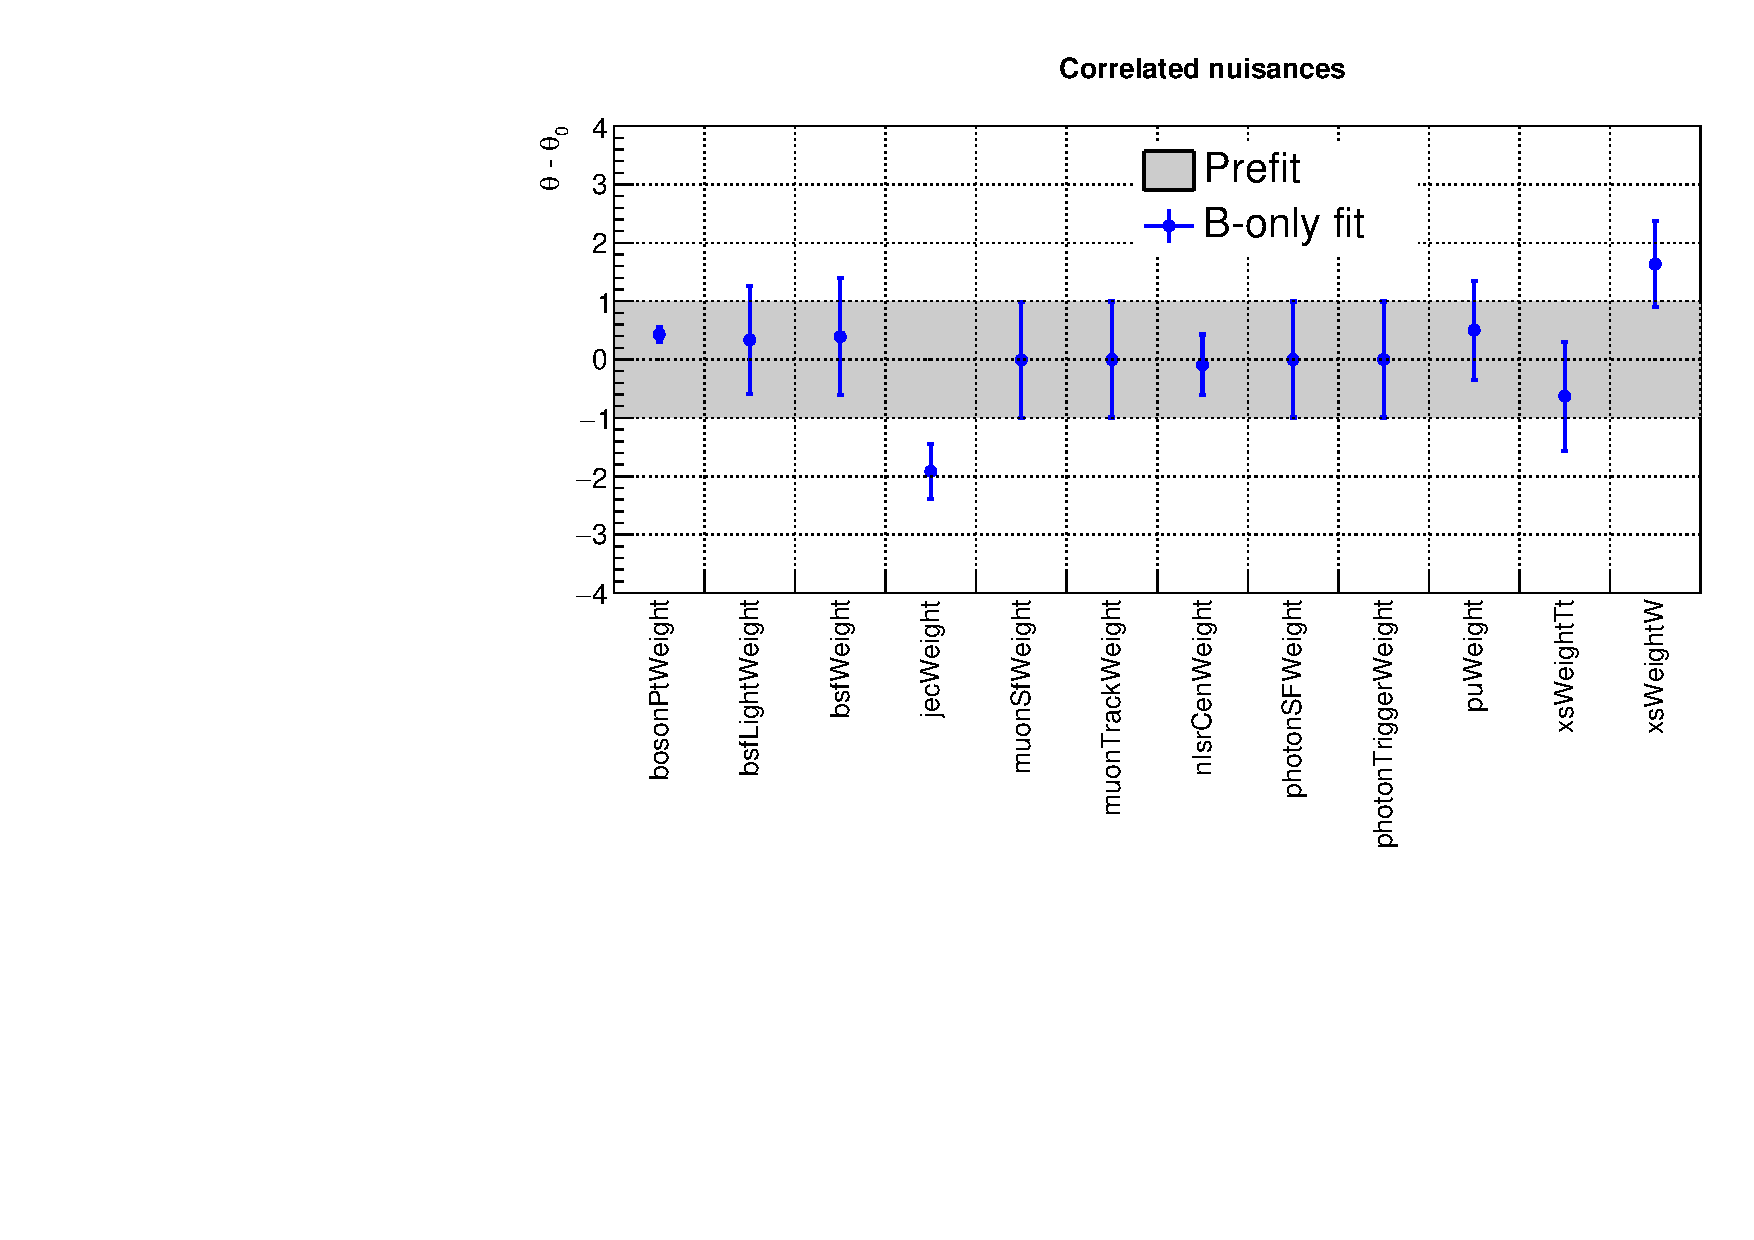
\includegraphics[width=0.45\textwidth]{figures/closureTests/AlphaT/AlphaT_Correlated_nuisances.pdf}
    \caption{The post-fit nuisance parameter values (relative to
      pre-fit) for the \alphat closure test when implemented as a
      binned likelihood fit.} 
    \label{fig:closure_AlphaT_LH_mu}
  \end{center} 
\end{figure}

\clearpage
\subsection{Extrapolation in \texorpdfstring{\bdphi}{biased dPhi}}

\begin{figure}[h!]
  \begin{center}
    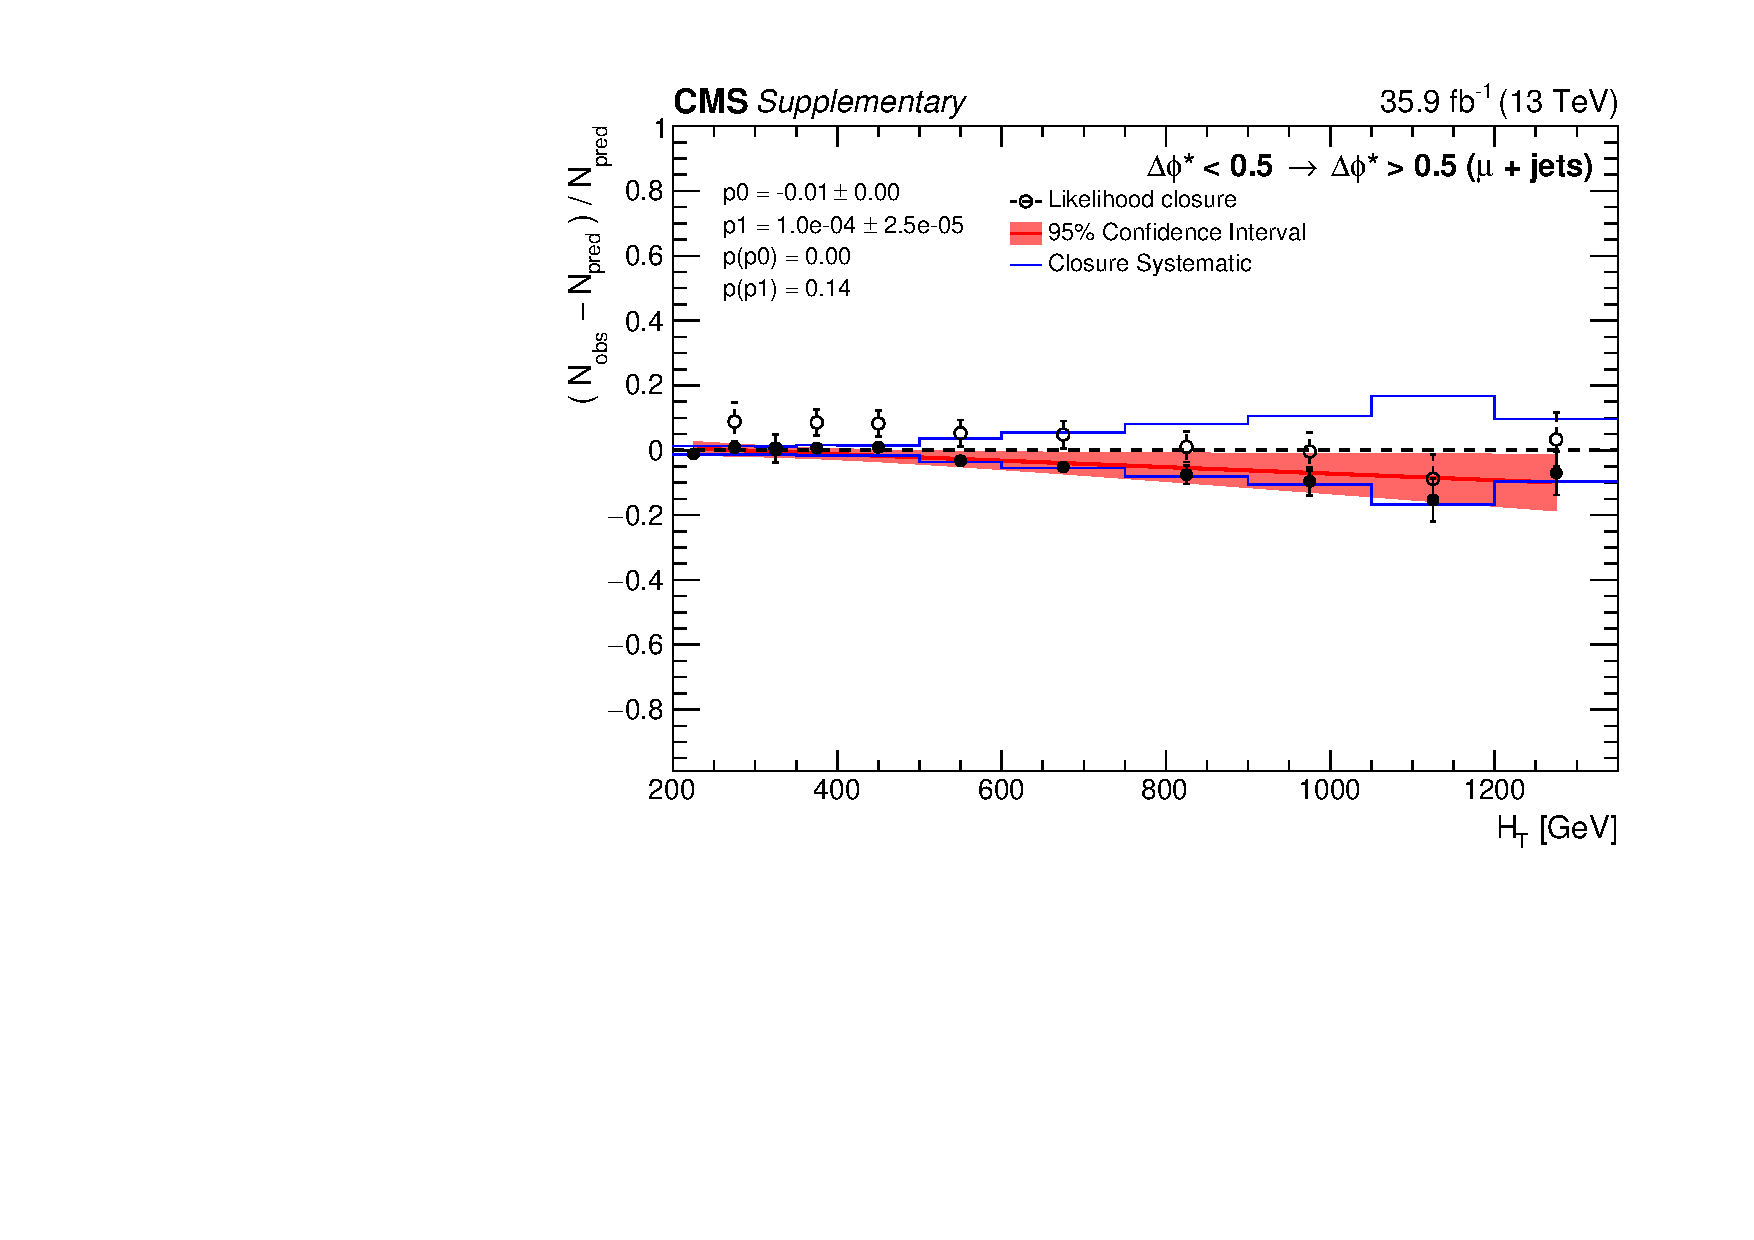
\includegraphics[width=0.45\textwidth]{figures/closureTests/bDPhi/SingleMu_bdphiExtrapolation_ht.pdf}~
    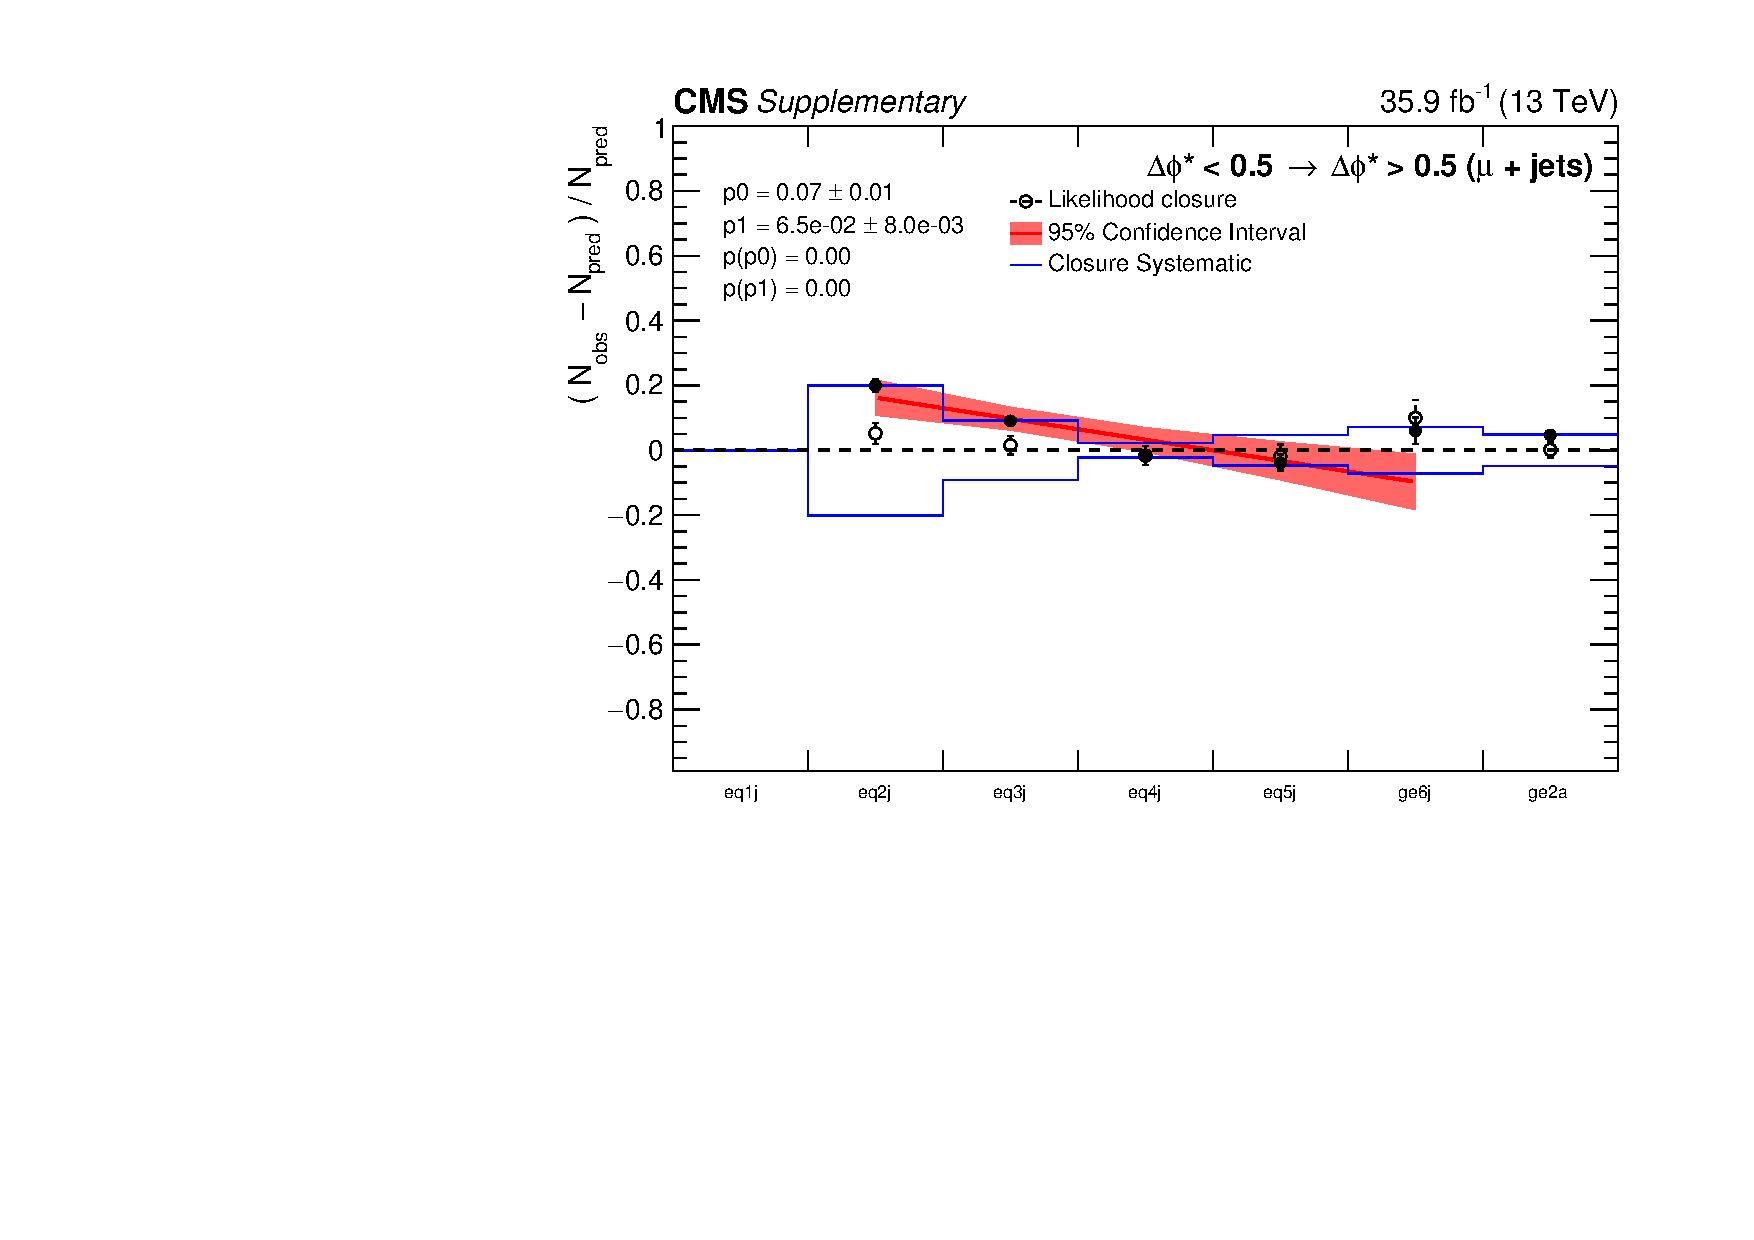
\includegraphics[width=0.45\textwidth]{figures/closureTests/bDPhi/SingleMu_bdphiExtrapolation_nJet.pdf}\\
    \caption{Data-driven closure tests probing the modelling of an
      extrapolation in the \bdphi variable with the \mj sample. The
      level of closure (solid markers) is indicated as a function of
      \scalht (left) and \njet (right). The blue histogram indicates
      the quadrature sum of the magnitude of non-closure and its
      statistical uncertainty. The post-fit closure (open markers) is
      also shown (see text for details).  }
    \label{fig:closure_bDPhi_mu}
  \end{center} 
\end{figure}

\begin{figure}[h!]
  \begin{center}
    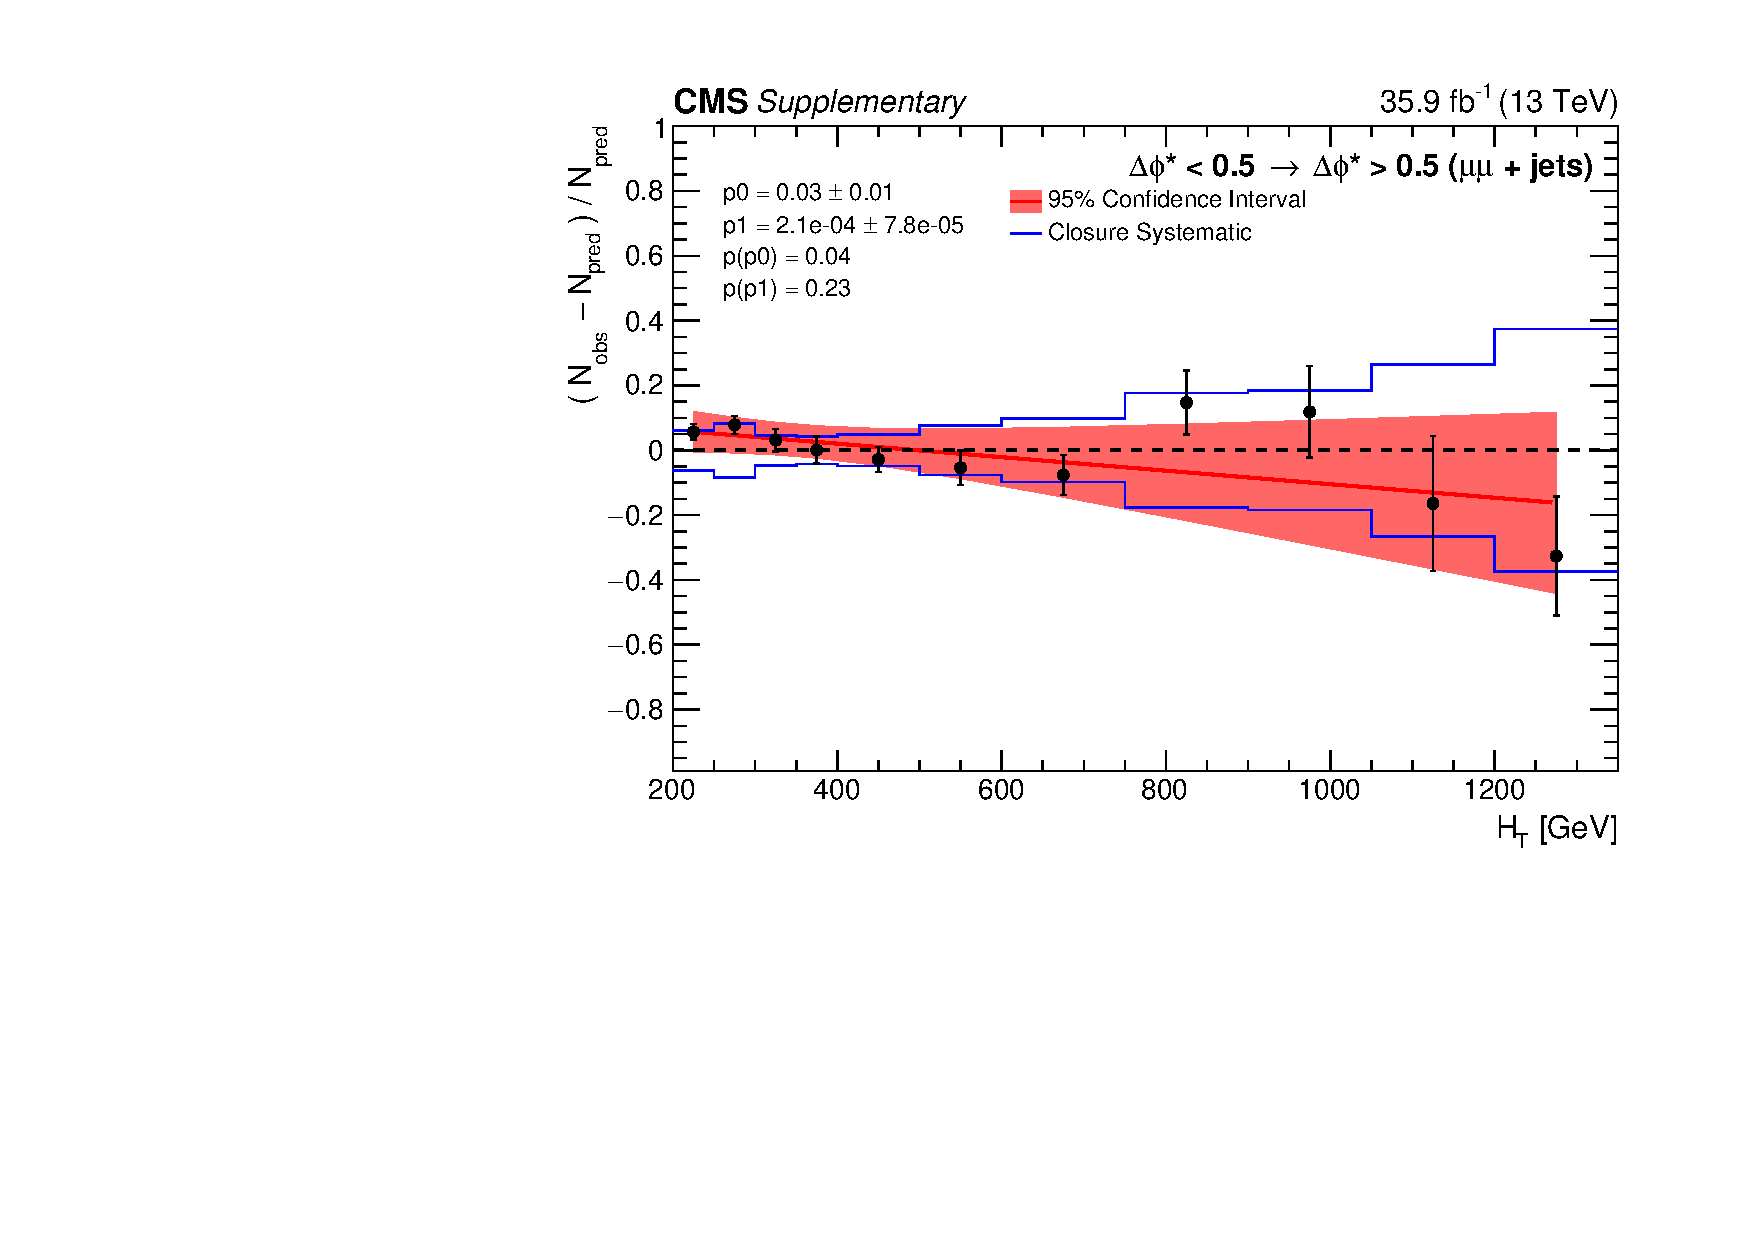
\includegraphics[width=0.45\textwidth]{figures/closureTests/bDPhi/DoubleMu_bdphiExtrapolation_ht.pdf}~
    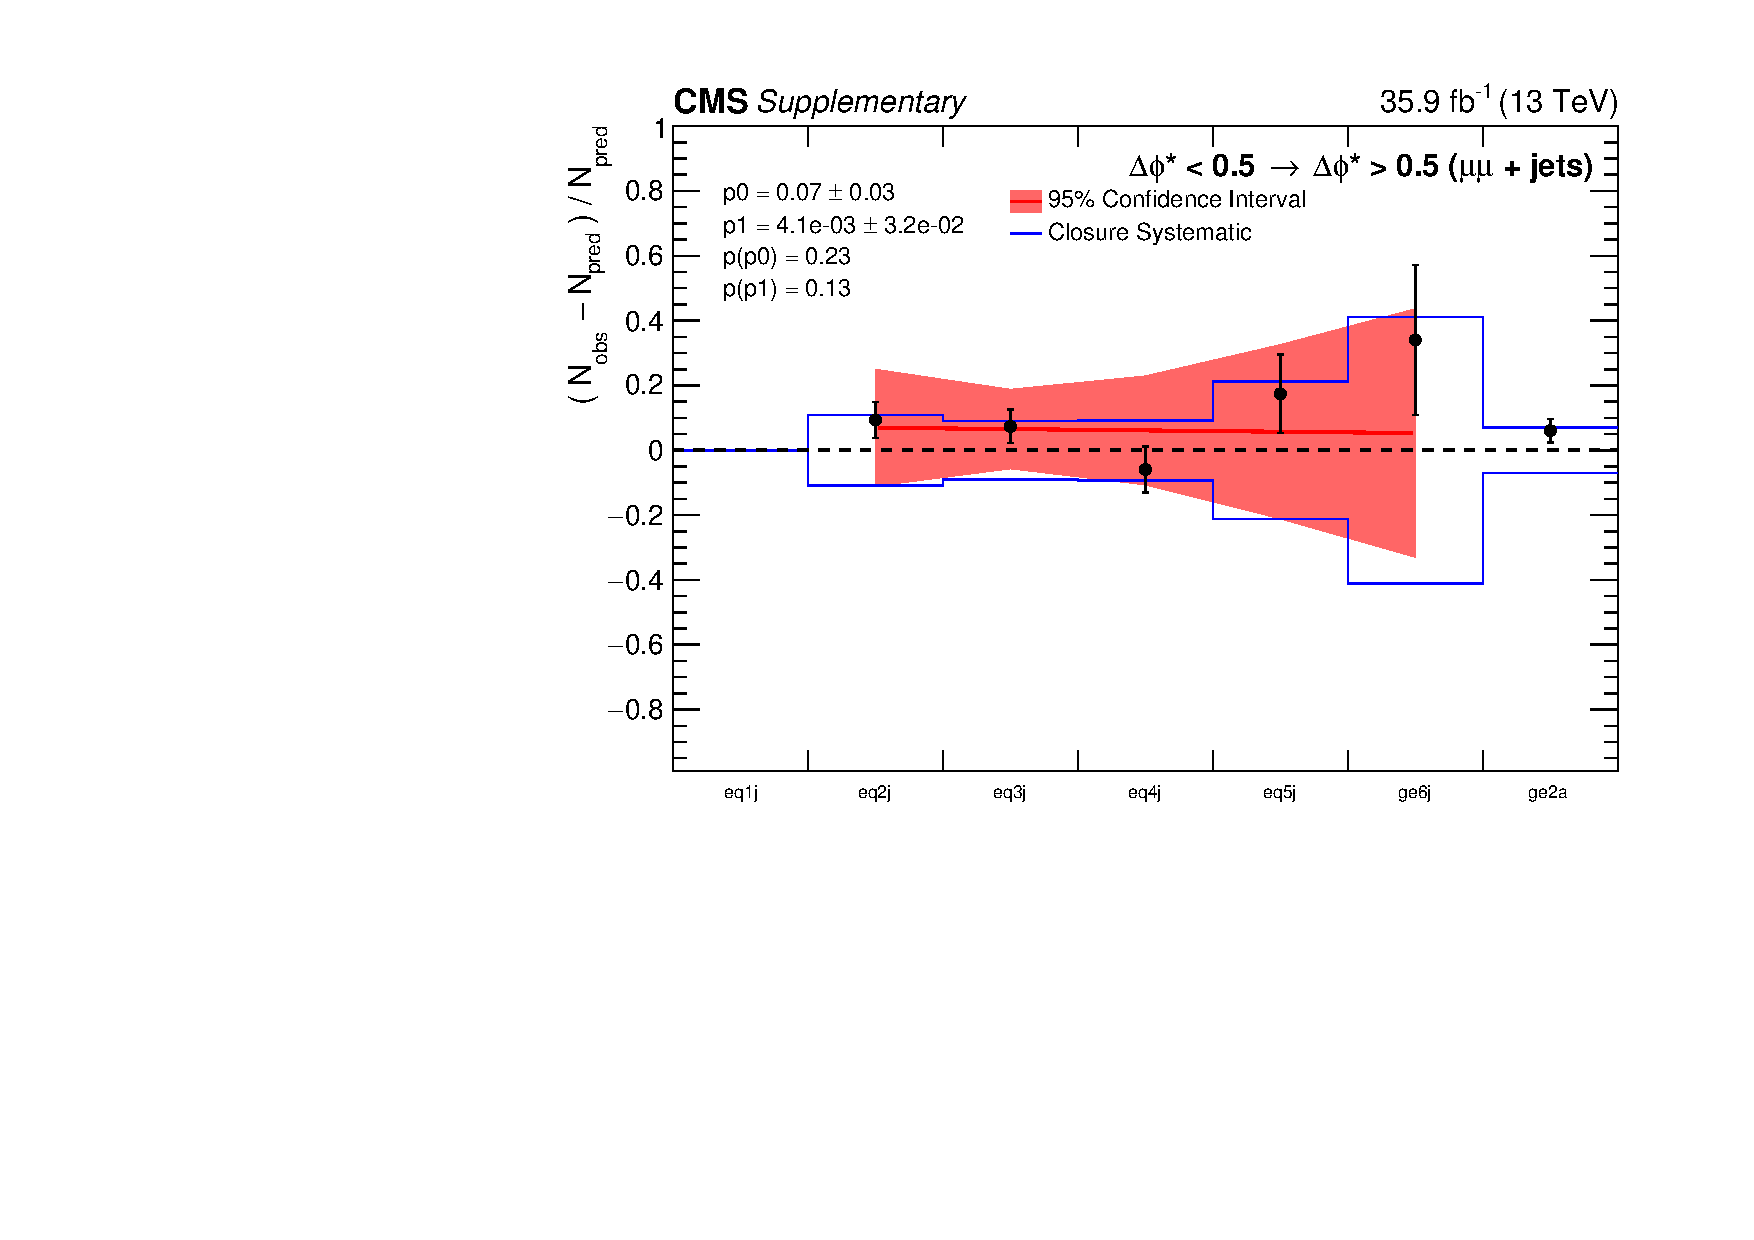
\includegraphics[width=0.45\textwidth]{figures/closureTests/bDPhi/DoubleMu_bdphiExtrapolation_nJet.pdf}\\ 
    \caption{As for Fig.~\ref{fig:closure_bDPhi_mu} but probing the
      modelling of an extrapolation in the \bdphi variable with the
      \mmj sample.
    }
    \label{fig:closure_bDPhi_mumu}
  \end{center} 
\end{figure}

\begin{figure}[h!]
  \begin{center}
    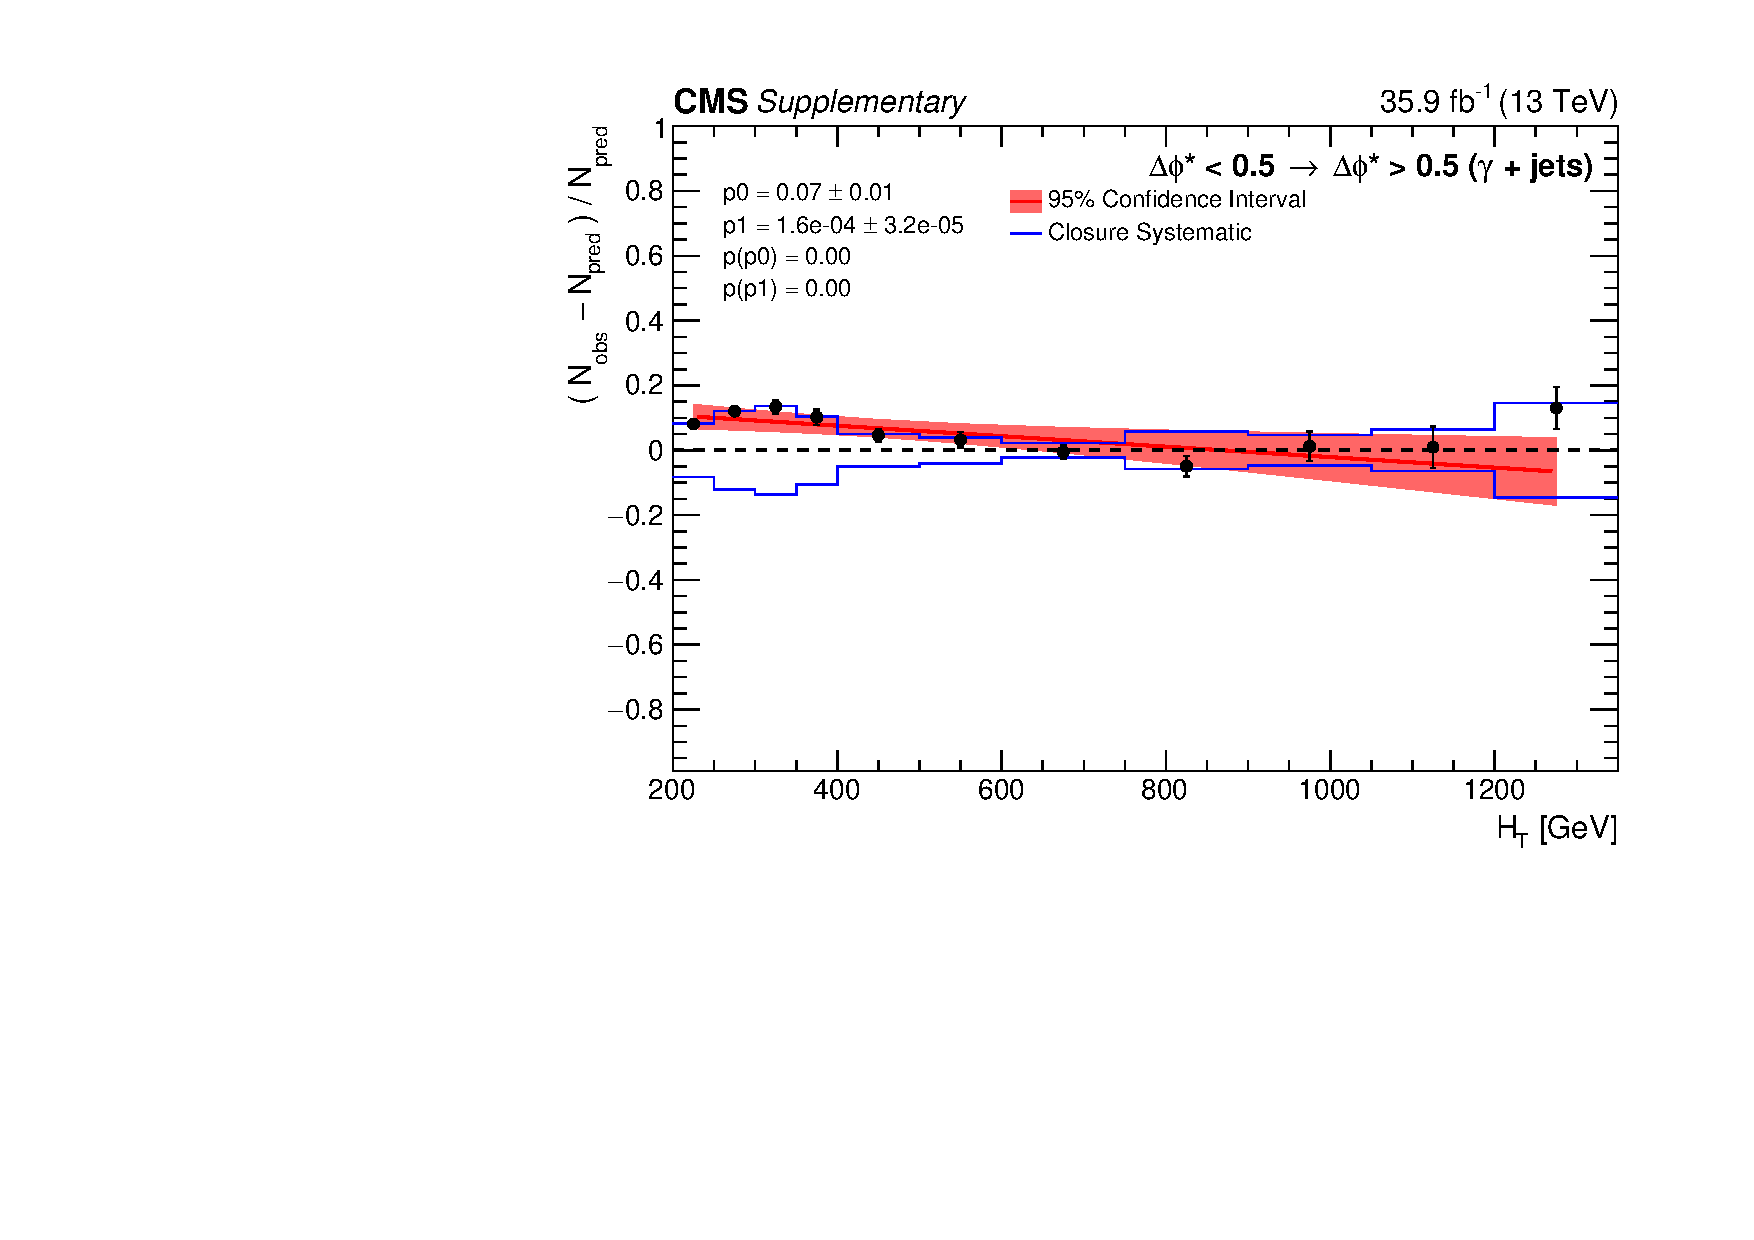
\includegraphics[width=0.45\textwidth]{figures/closureTests/bDPhi/SinglePhoton_bdphiExtrapolation_ht.pdf}~
    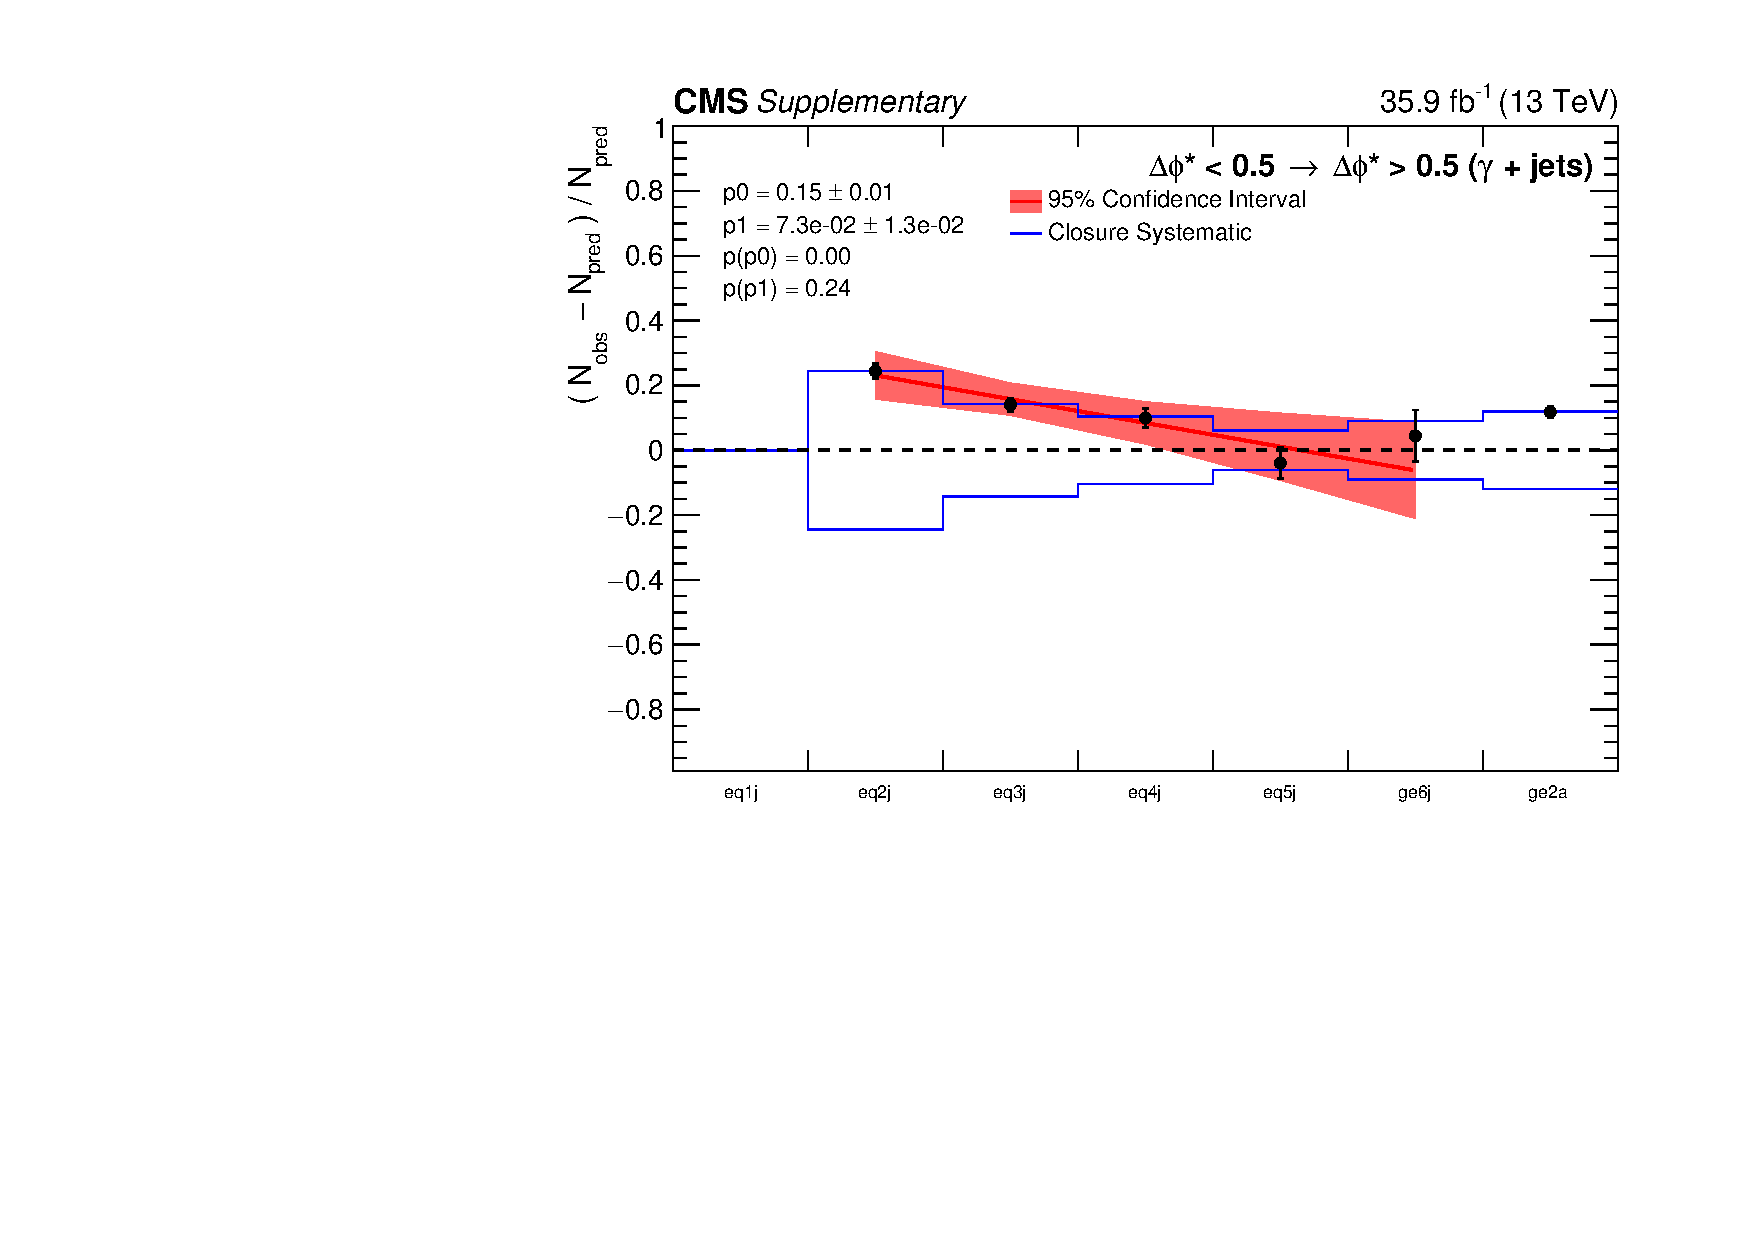
\includegraphics[width=0.45\textwidth]{figures/closureTests/bDPhi/SinglePhoton_bdphiExtrapolation_nJet.pdf}\\ 
    \caption{As for Fig.~\ref{fig:closure_bDPhi_mu} but probing the
      modelling of an extrapolation in the \bdphi variable with the
      \gj sample.
    }
    \label{fig:closure_bDPhi_phot}
  \end{center} 
\end{figure}

\clearpage
\subsection{Extrapolation in \texorpdfstring{\alphat}{AlphaT} and
  \texorpdfstring{\bdphi}{biased dPhi}}

\begin{figure}[h!]
  \begin{center}
    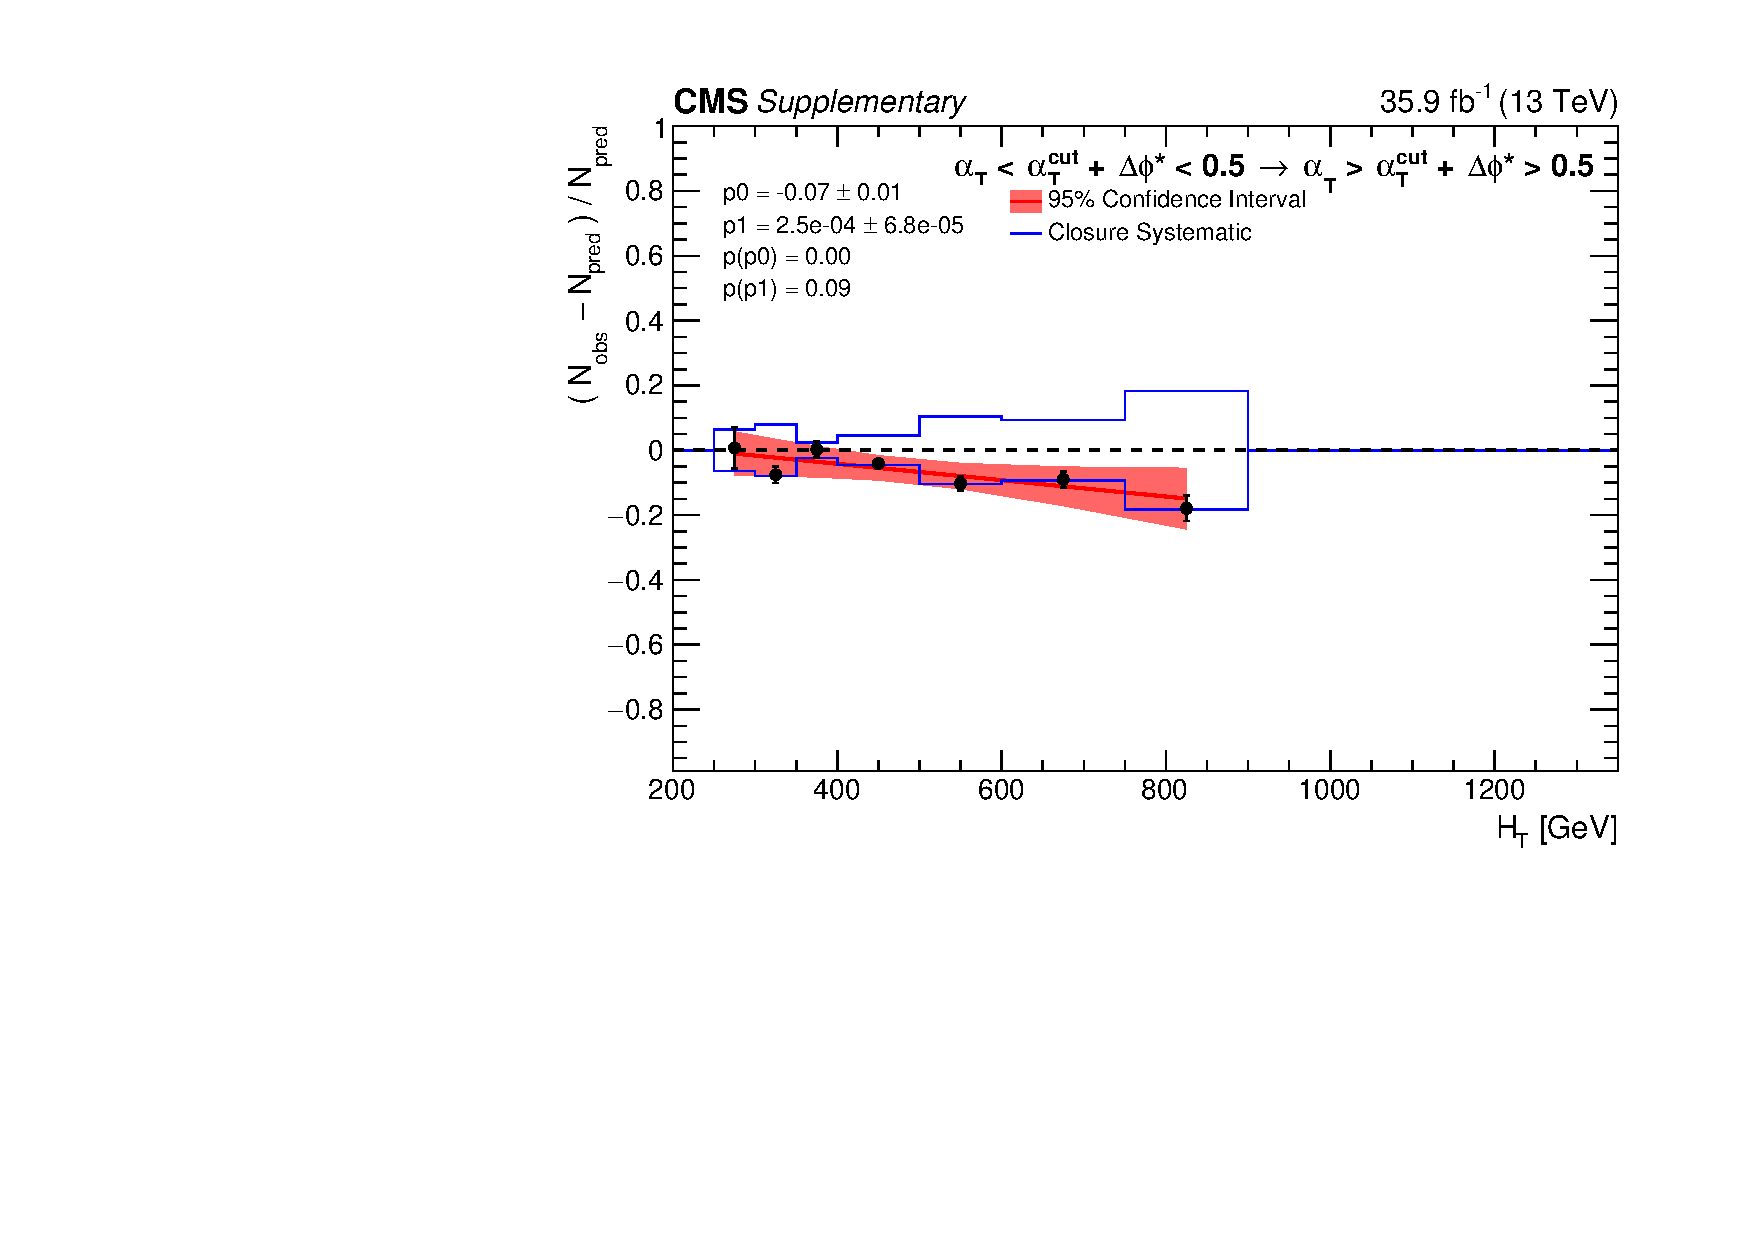
\includegraphics[width=0.45\textwidth]{figures/closureTests/AlphaT_bDPhi/SingleMu_alphaTbdphi_ht.pdf}~
    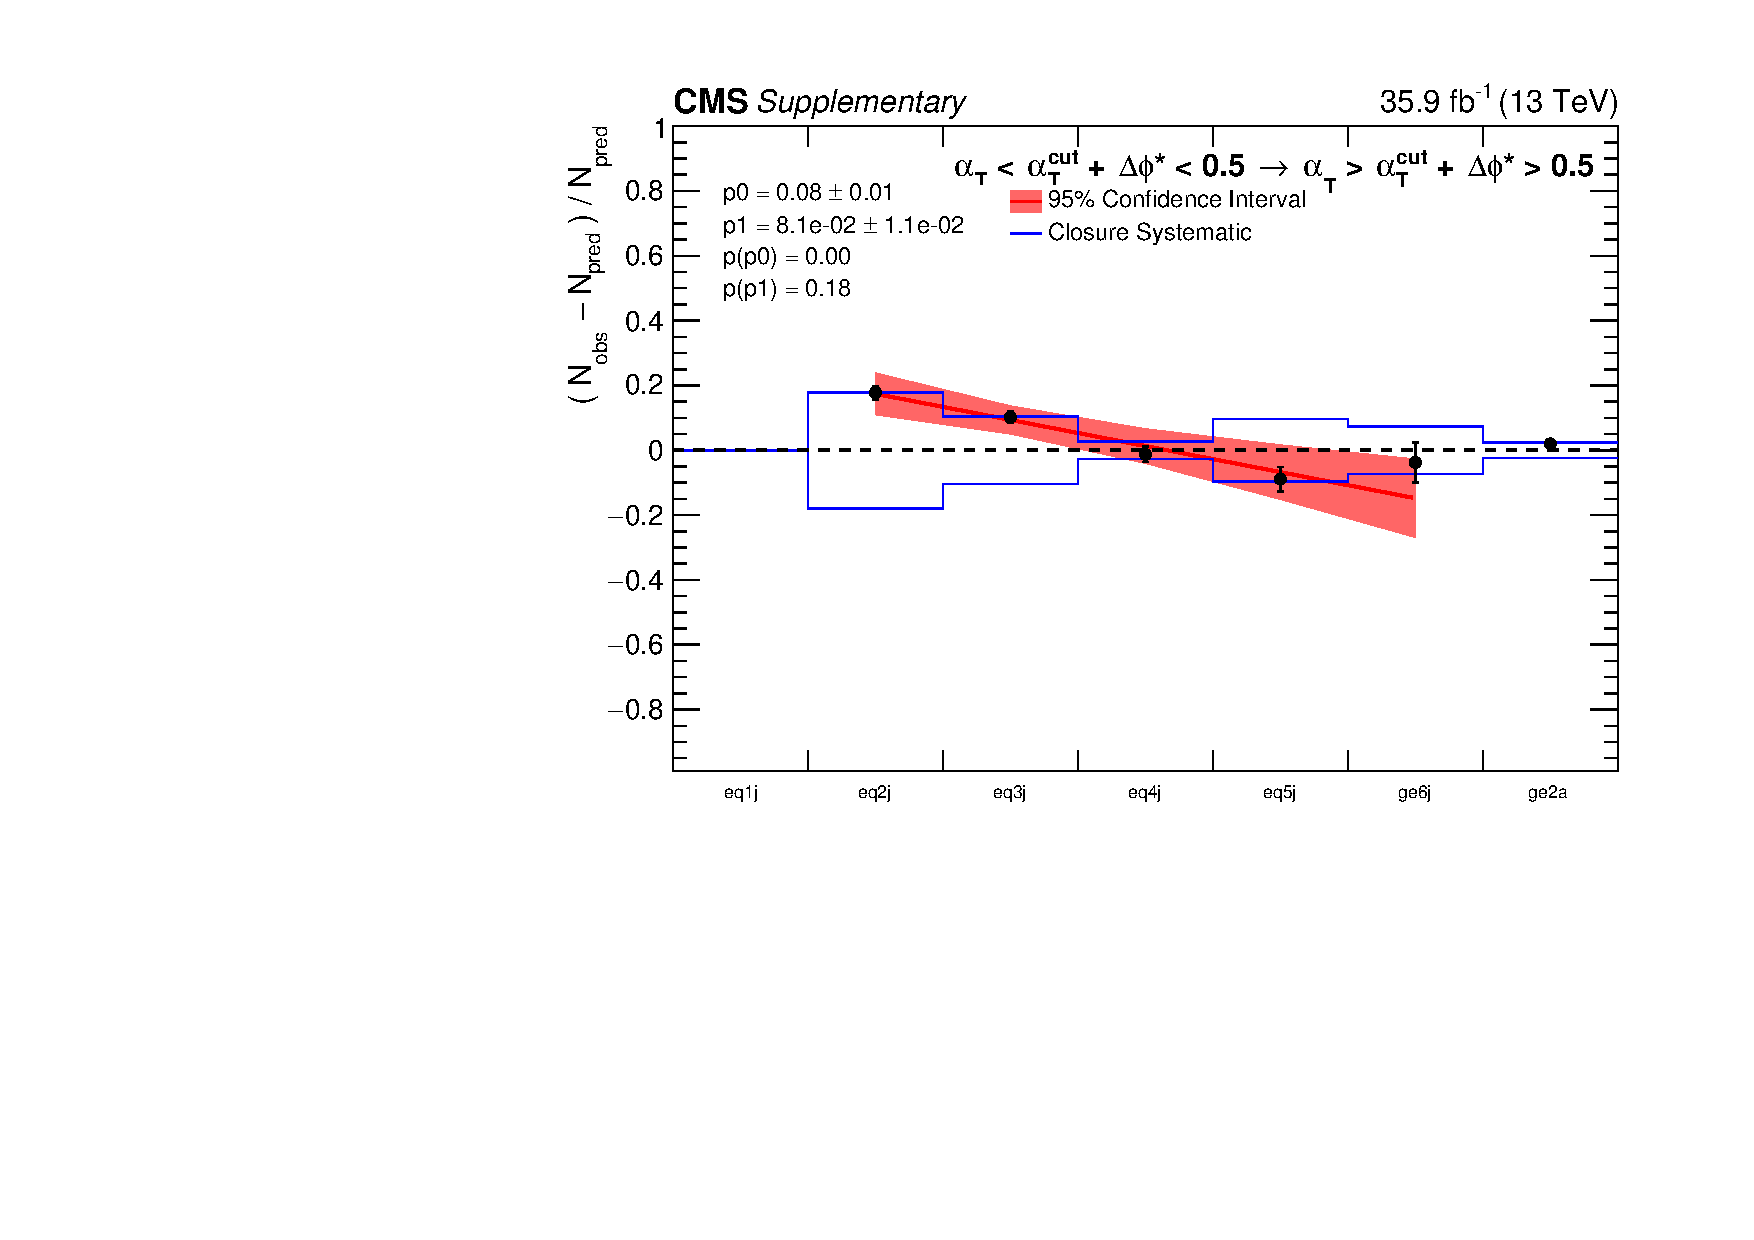
\includegraphics[width=0.45\textwidth]{figures/closureTests/AlphaT_bDPhi/SingleMu_alphaTbdphi_nJet.pdf}\\
    \caption{Data-driven closure tests probing the modelling of an
      extrapolation in both \alphat and \bdphi variables, as done in
      the analysis, with the \mj sample. The level of closure (solid
      markers) is indicated as a function of \scalht (left) and \njet
      (right). The blue histogram indicates the quadrature sum of the
      magnitude of non-closure and its statistical uncertainty. The
      post-fit closure (open markers) is also shown (see text for
      details). \fixme{UPDATE PLOTS WITH CLOSURE FIT!} }
    \label{fig:closure_AlphaT_bDPhi_mu}
  \end{center} 
\end{figure}

\begin{figure}[h!]
  \begin{center}
    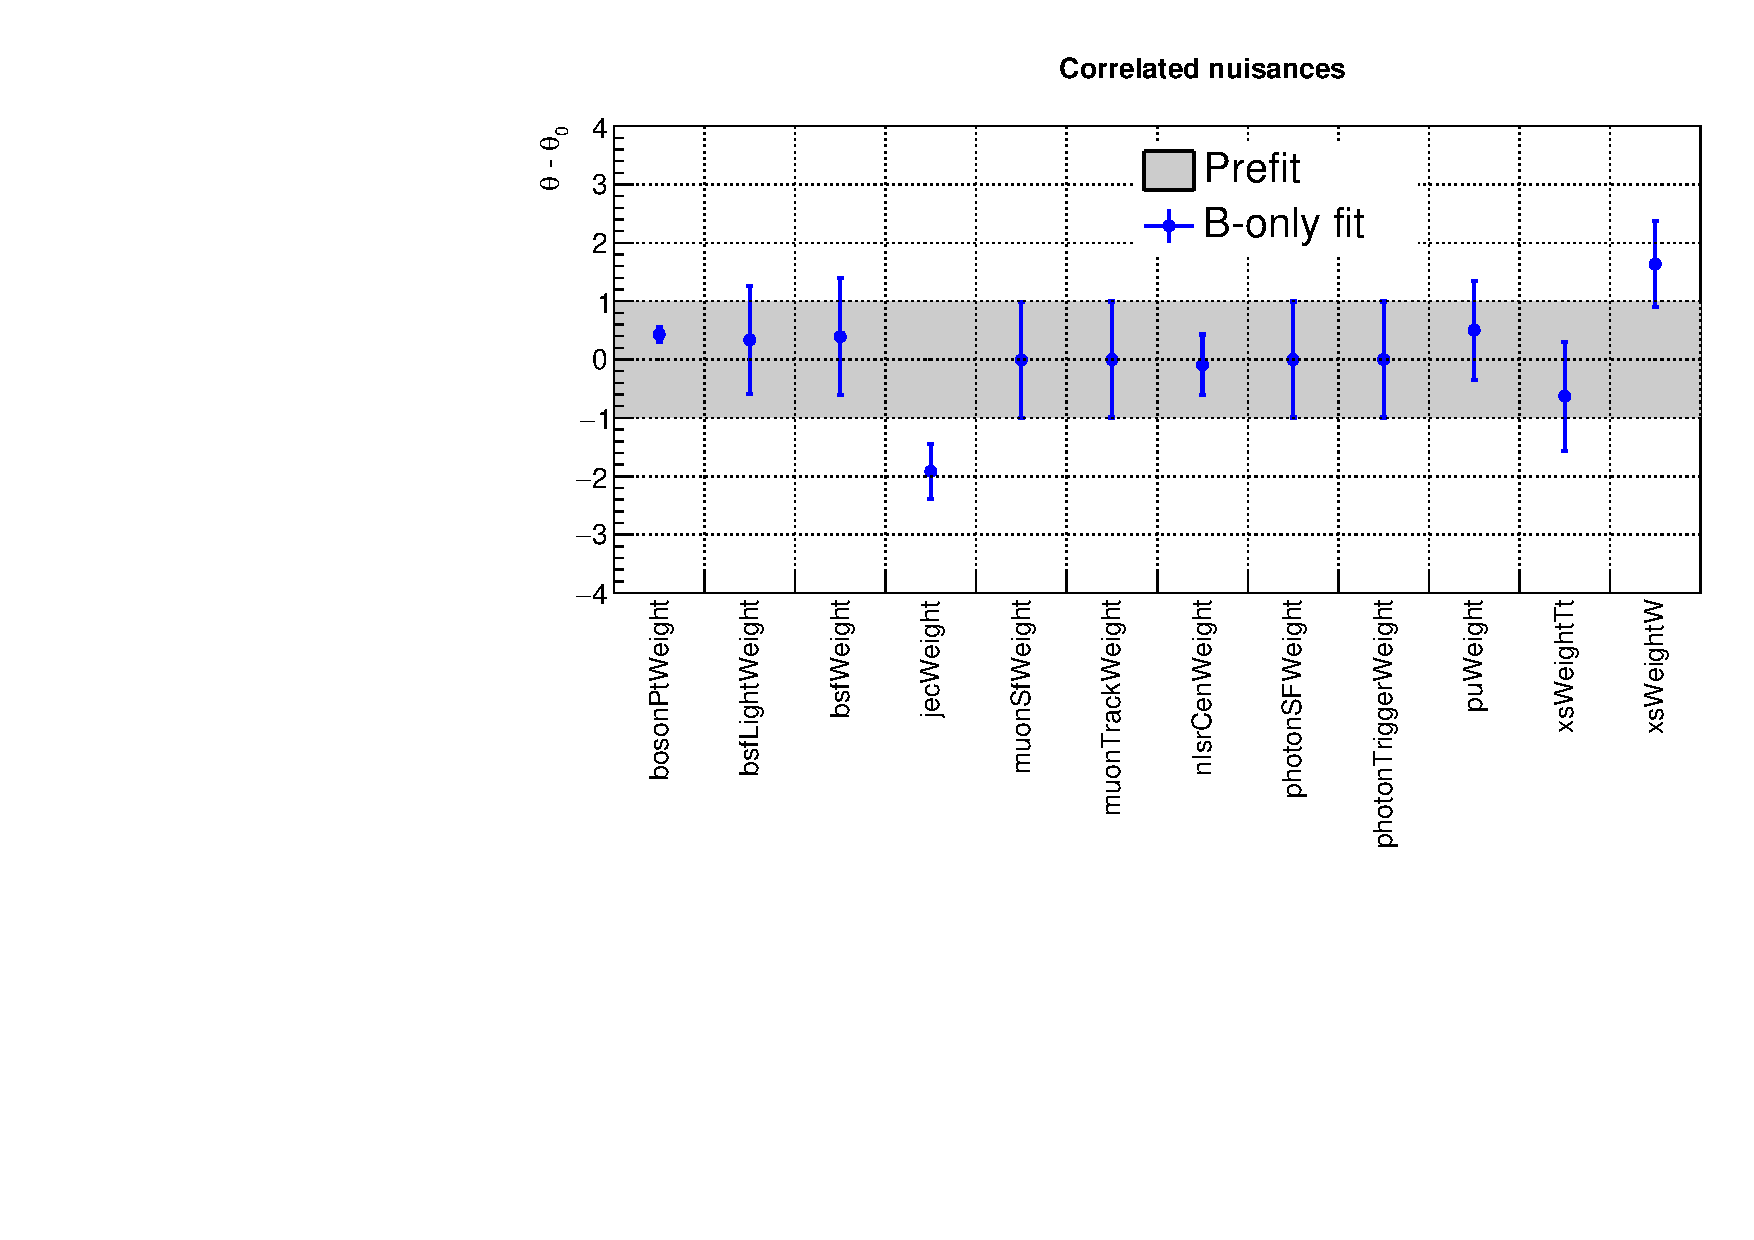
\includegraphics[width=0.45\textwidth]{figures/closureTests/AlphaT/AlphaT_Correlated_nuisances.pdf}
    \caption{The post-fit nuisance parameter values (relative to
      pre-fit) for the combined \alphat and \bdphi closure test when
      implemented as a binned likelihood fit. \fixme{UPDATE PLOT!!!}} 
    \label{fig:closure_AlphaT_bDPhi_LH_mu}
  \end{center} 
\end{figure}

\clearpage
\subsection{The effect of W polarisation on lepton acceptance}

\begin{figure}[h!]
  \begin{center}
    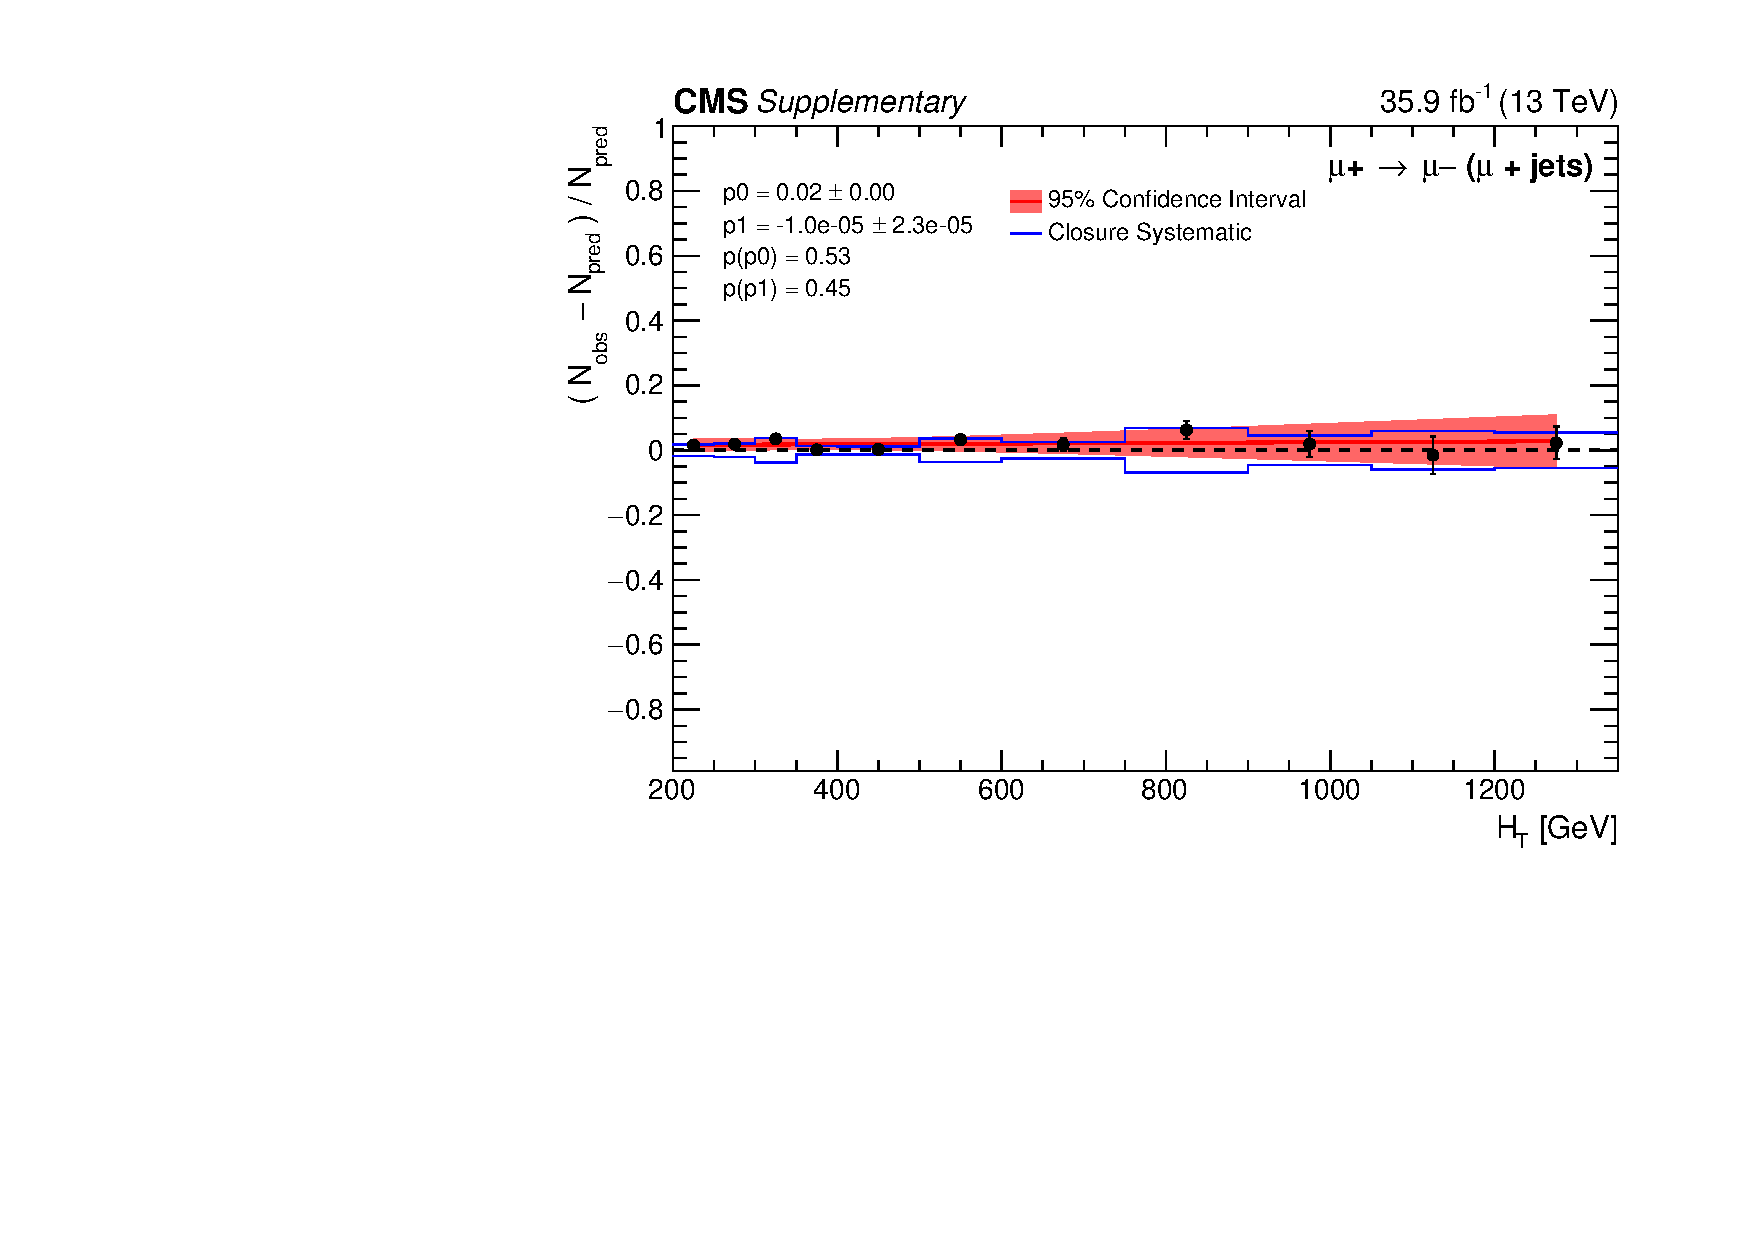
\includegraphics[width=0.45\textwidth]{figures/closureTests/WPol/SingleMuPlus_to_SingleMuMinus_ht.pdf}~
    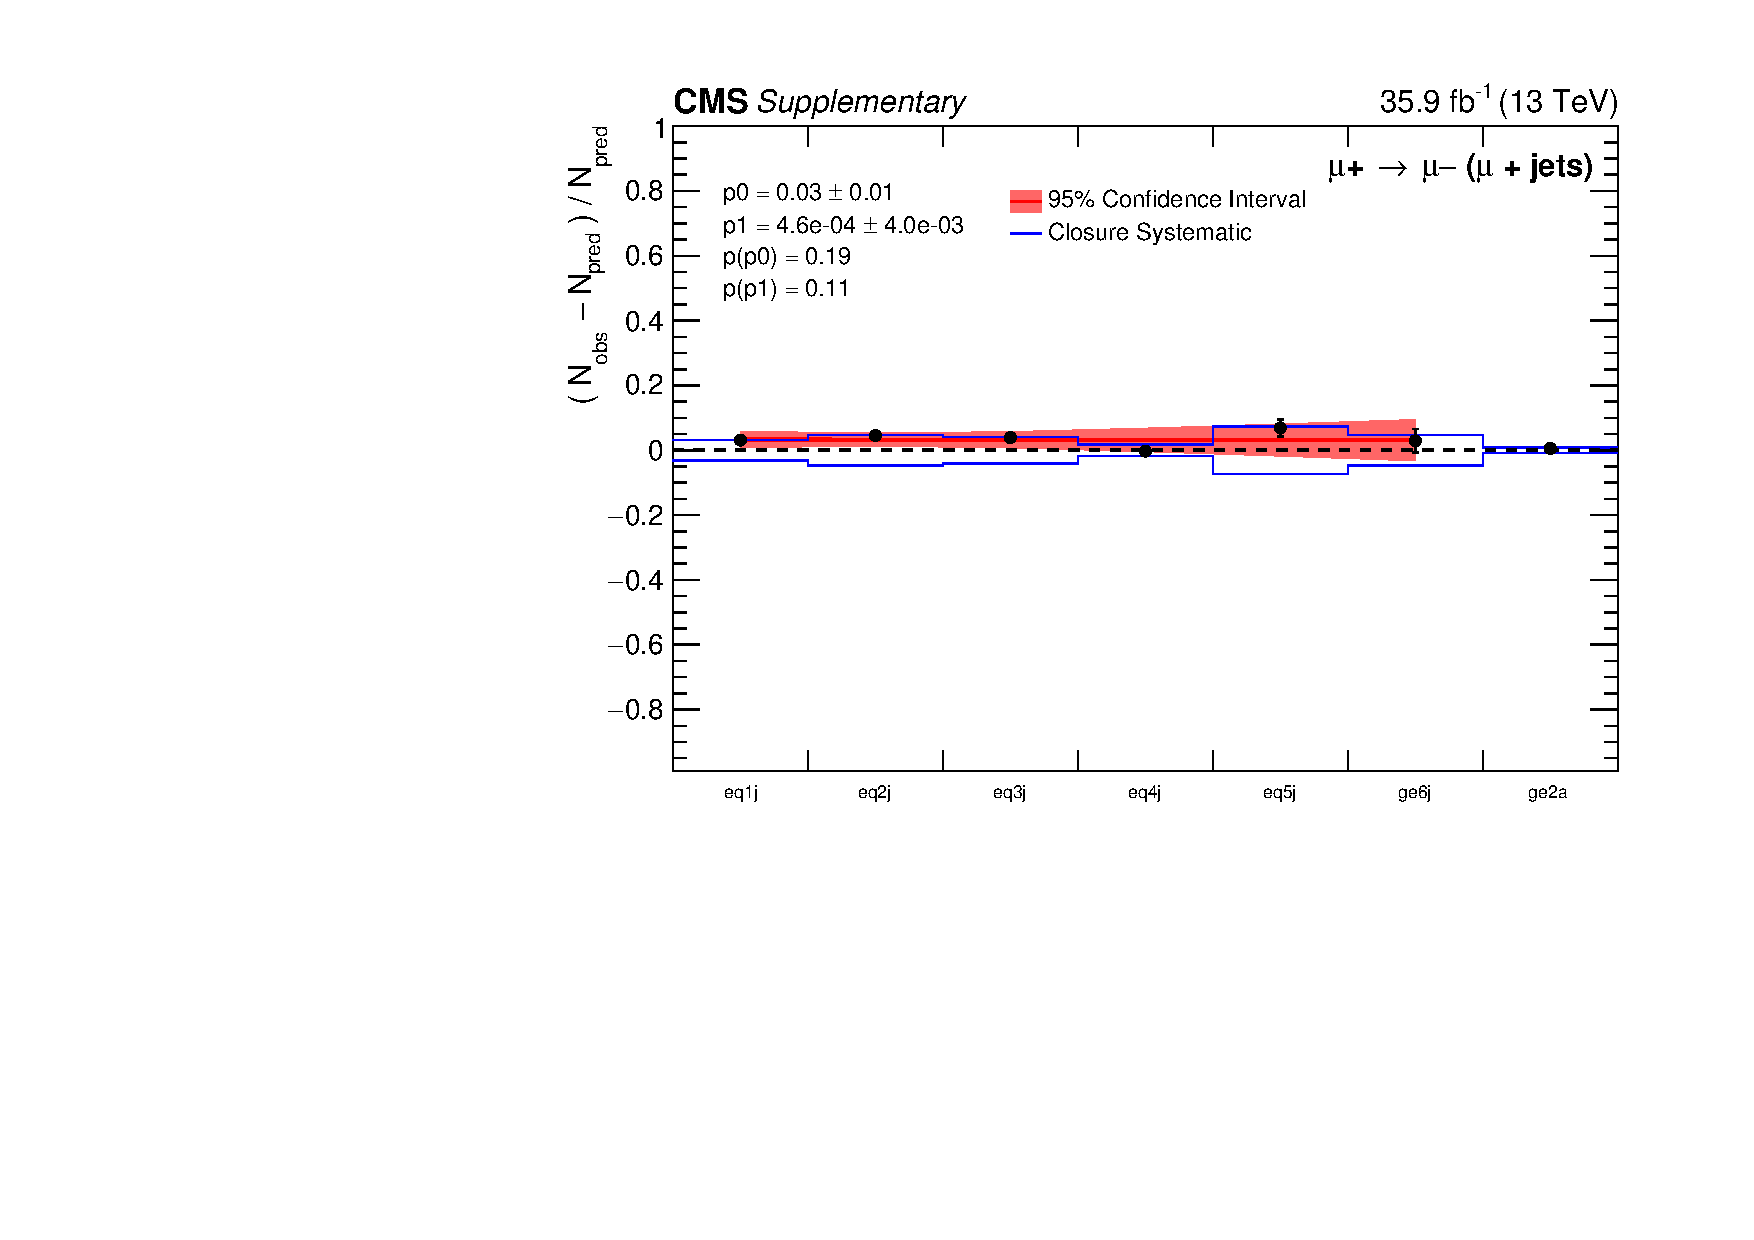
\includegraphics[width=0.45\textwidth]{figures/closureTests/WPol/SingleMuPlus_to_SingleMuMinus_nJet.pdf}\\
    \caption{Data-driven closure tests that probe the modelling of W
      polarisation in the \mj sample. The level of closure (solid
      markers) is indicated as a function of \scalht (left) and \njet
      (right). The blue histogram indicates the quadrature sum of the
      magnitude of non-closure and its statistical uncertainty. }
    \label{fig:closure_WPol_mu}
  \end{center} 
\end{figure}

\clearpage
\subsection{The single isolated track veto}

\begin{figure}[h!]
  \begin{center}
    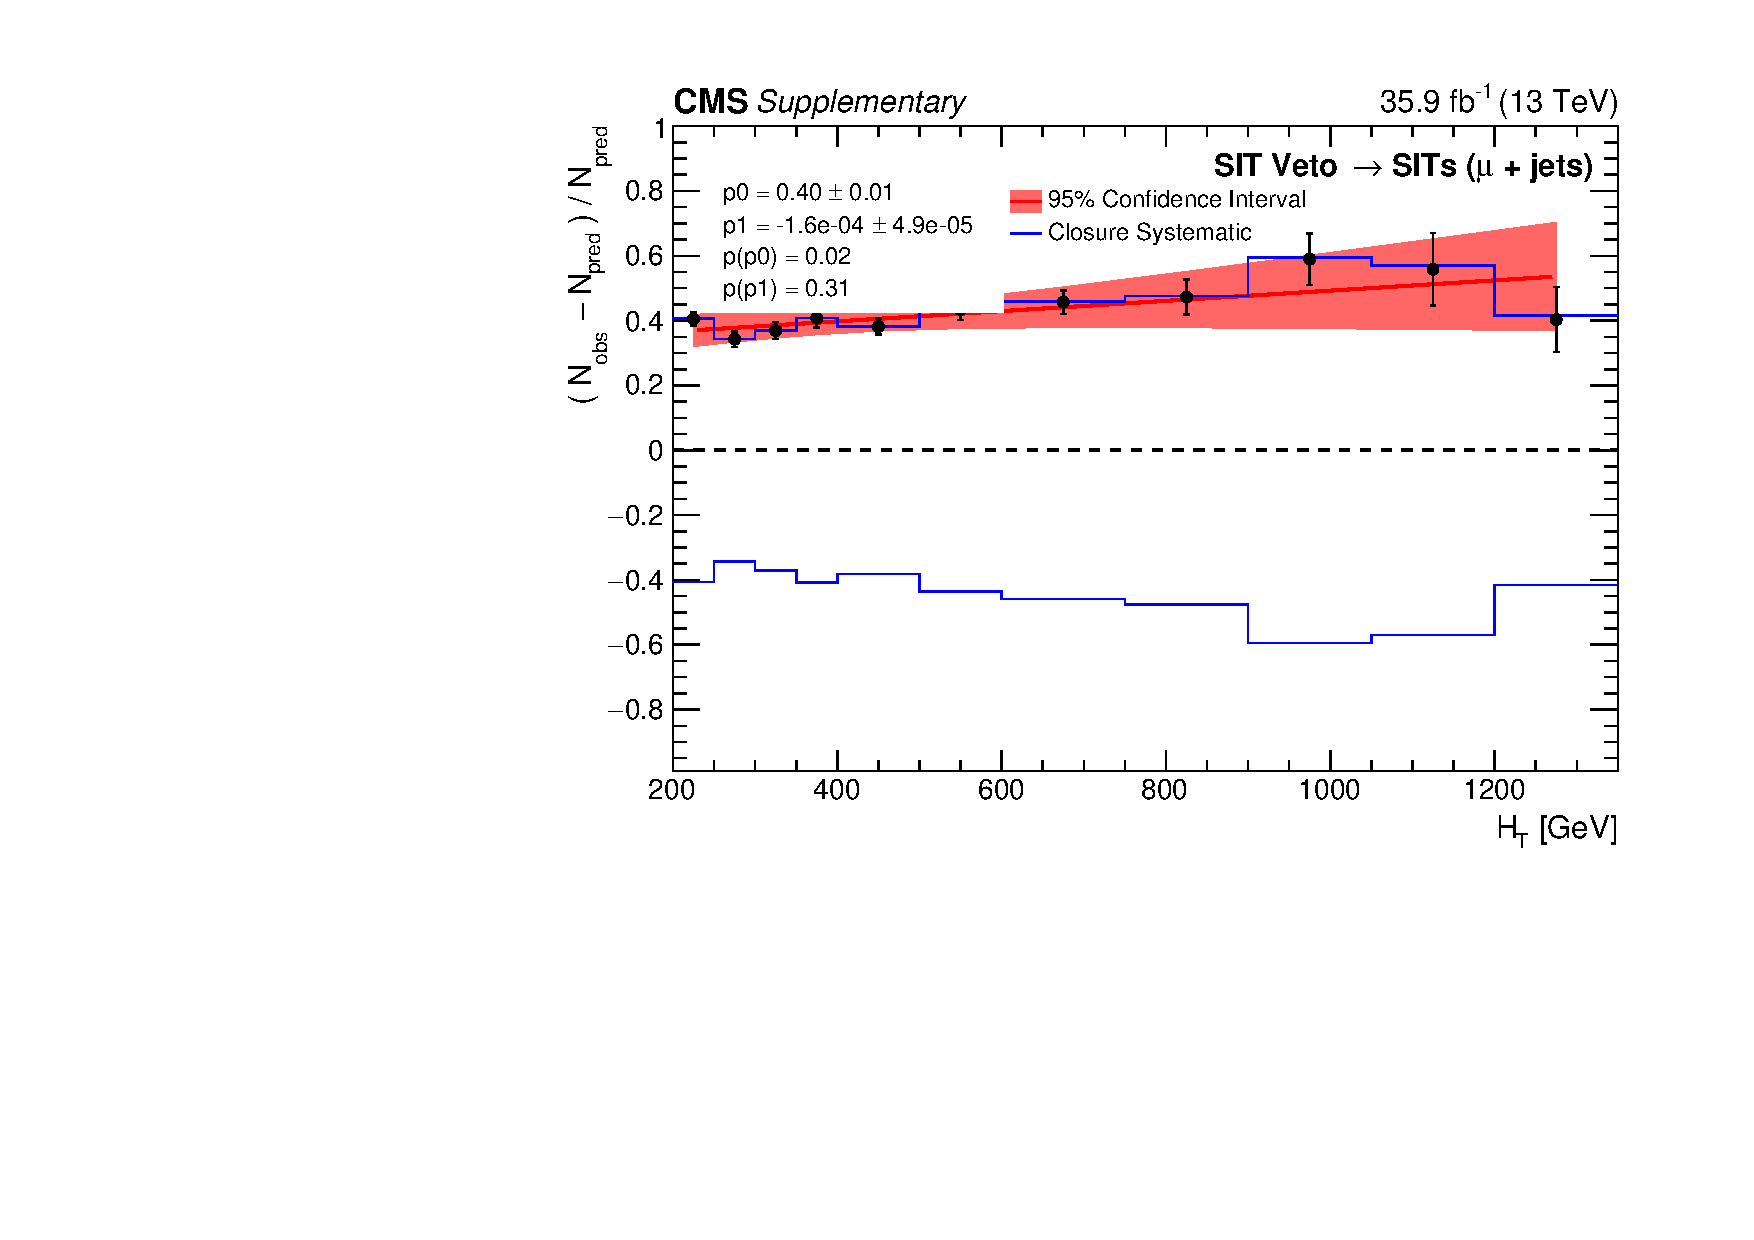
\includegraphics[width=0.45\textwidth]{figures/closureTests/SITV/SingleMu_Sit_ht.pdf}~
    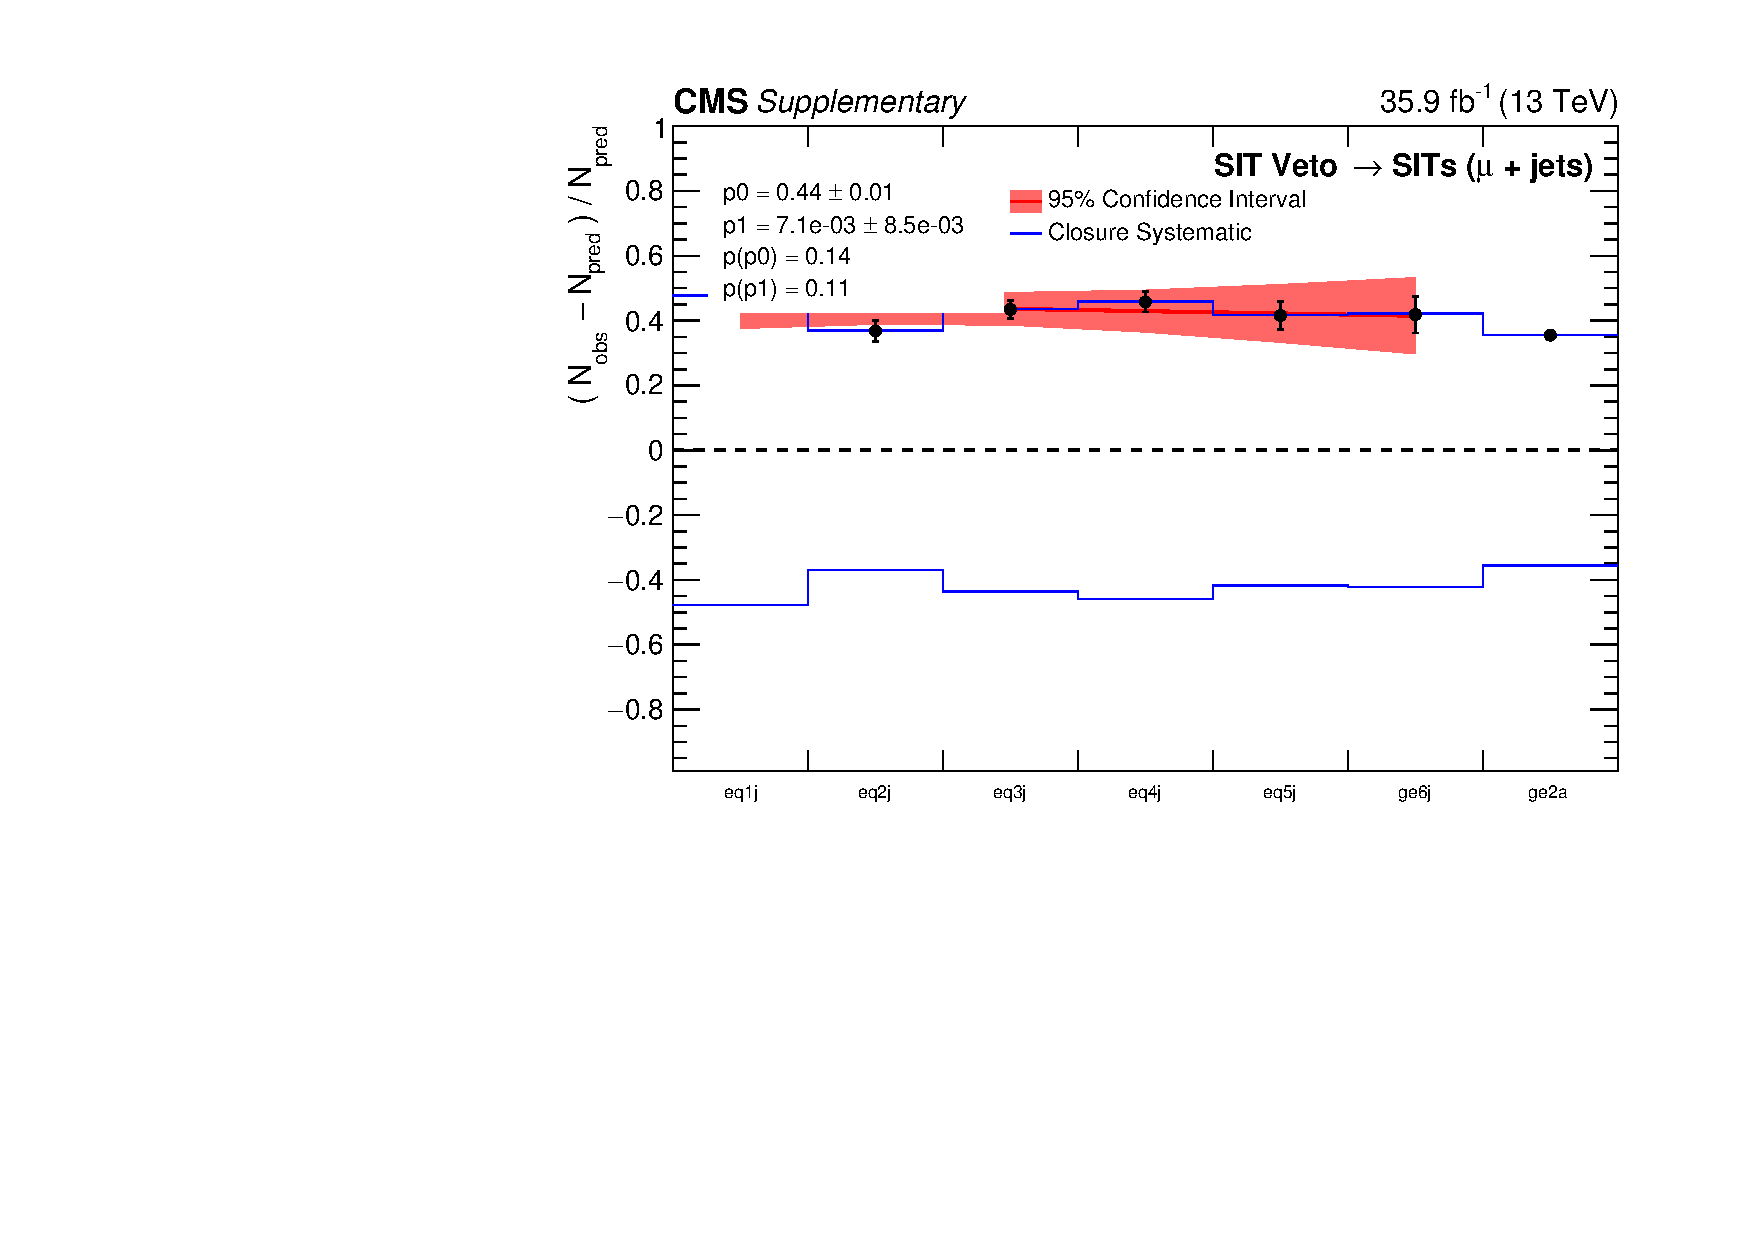
\includegraphics[width=0.45\textwidth]{figures/closureTests/SITV/SingleMu_Sit_nJet.pdf}\\
    \caption{Data-driven closure tests that probe the modelling of the
      single isolated track veto. The level of closure (solid markers)
      is indicated as a function of \scalht (left) and \njet
      (right). The blue histogram indicates the quadrature sum of the
      magnitude of non-closure and its statistical uncertainty. }
    \label{fig:closure_SITV_mu}
  \end{center} 
\end{figure}

\clearpage
\begin{figure}[h!]
  \begin{center}
    \includegraphics[width=0.3\textwidth,page=10,trim=0 100 50 100,clip]{figures/SITV/SIT/SIT.pdf}~
    \includegraphics[width=0.3\textwidth,page=6,trim=0 100 50 100,clip]{figures/SITV/SIT/SIT.pdf}~
    \includegraphics[width=0.3\textwidth,page=5,trim=0 100 50 100,clip]{figures/SITV/SIT/SIT.pdf}\\
    \includegraphics[width=0.3\textwidth,page=8,trim=0 100 50 100,clip]{figures/SITV/SIT/SIT.pdf}~
    \includegraphics[width=0.3\textwidth,page=4,trim=0 100 50 100,clip]{figures/SITV/SIT/SIT.pdf}~
    \includegraphics[width=0.3\textwidth,page=7,trim=0 100 50 100,clip]{figures/SITV/SIT/SIT.pdf}\\
    \includegraphics[width=0.3\textwidth,page=2,trim=0 100 50 100,clip]{figures/SITV/SIT/SIT.pdf}~
    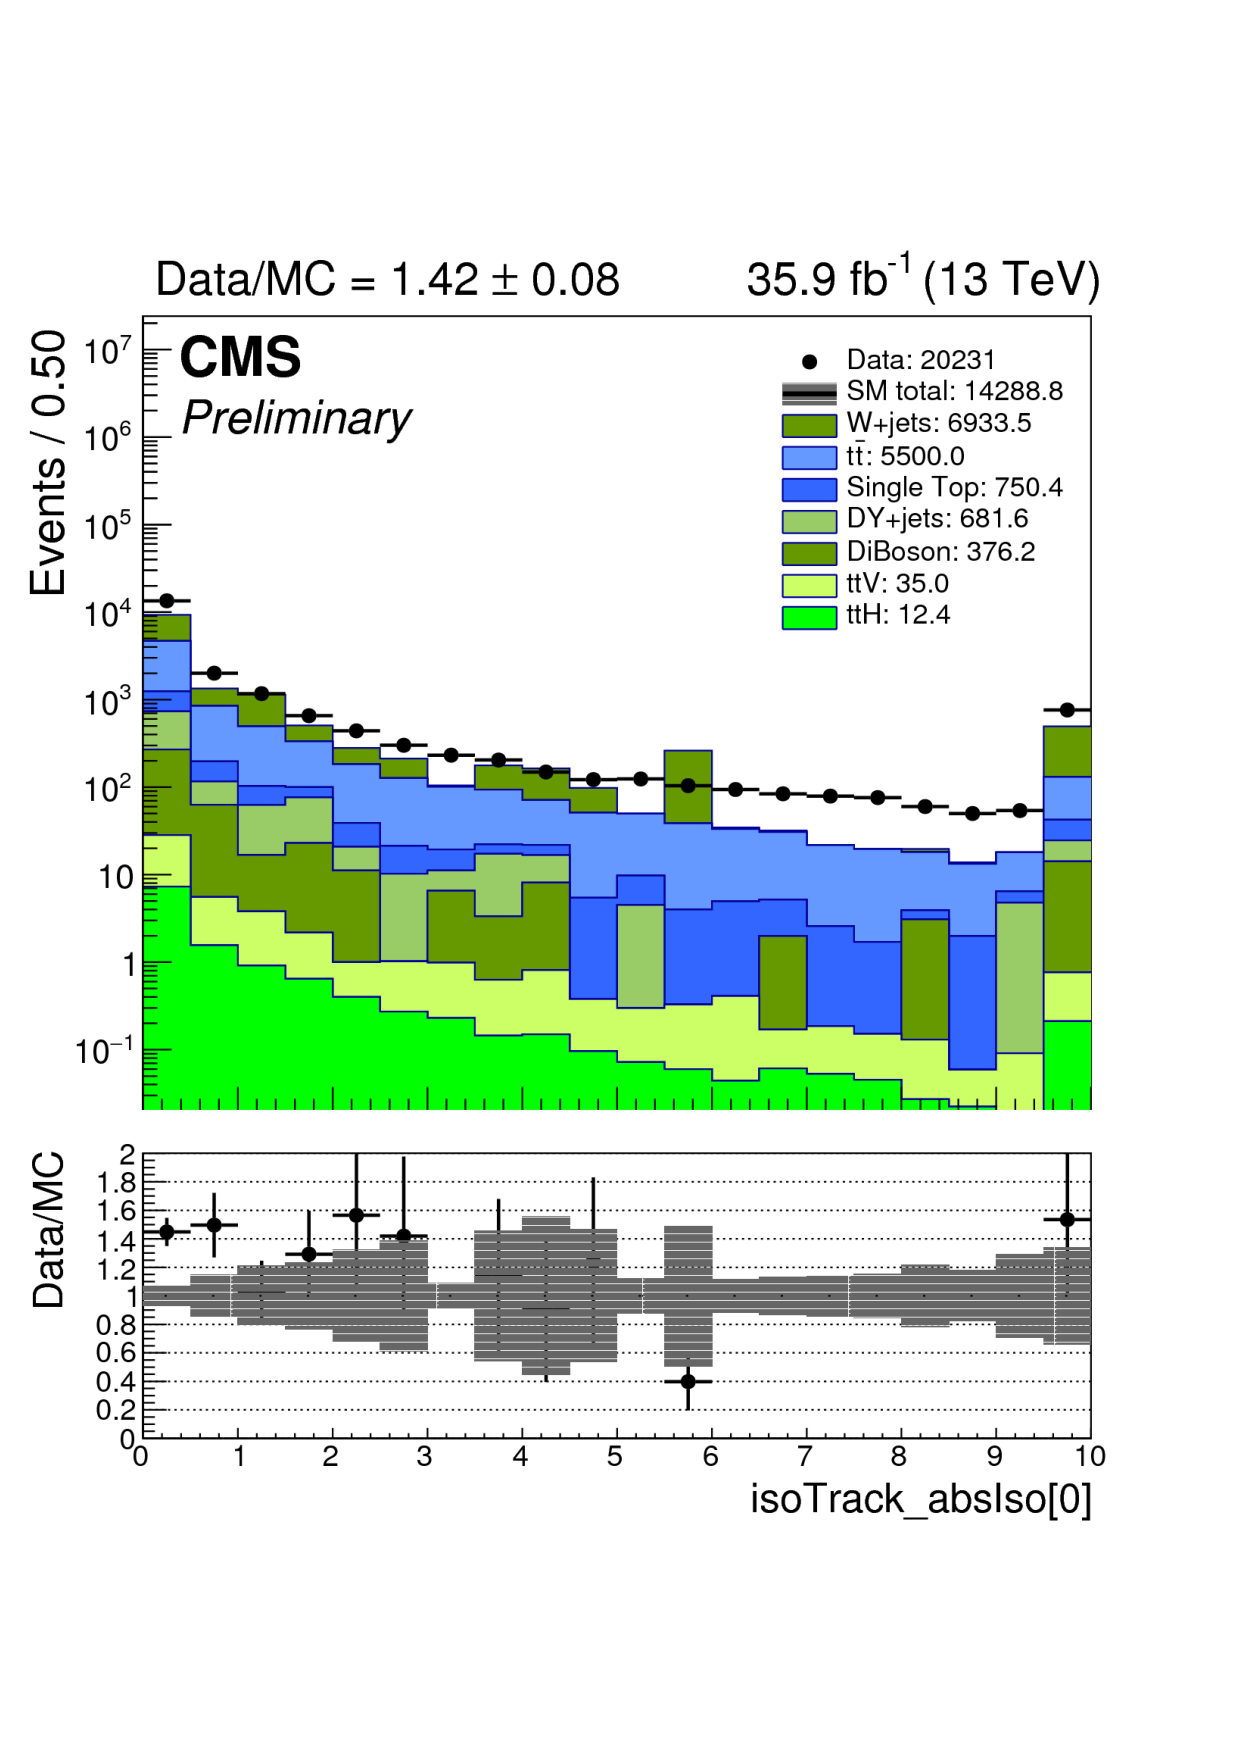
\includegraphics[width=0.3\textwidth,page=1,trim=0 100 50 100,clip]{figures/SITV/SIT/SIT.pdf}~
    \includegraphics[width=0.3\textwidth,page=9,trim=0 100 50 100,clip]{figures/SITV/SIT/SIT.pdf}\\
    \includegraphics[width=0.3\textwidth,page=3,trim=0 100 50 100,clip]{figures/SITV/SIT/SIT.pdf}~
    \caption{Distributions of various quantities related to SITs
      within a sample of \mj events containing at least SIT.}
    \label{fig:dataMC_SIT_mu}
  \end{center} 
\end{figure}

\clearpage
\begin{figure}[h!]
  \begin{center}
    \includegraphics[width=0.3\textwidth,page=18,trim=0 100 50 100,clip]{figures/SITV/Event/Event.pdf}~
    \includegraphics[width=0.3\textwidth,page=17,trim=0 100 50 100,clip]{figures/SITV/Event/Event.pdf}~
    \includegraphics[width=0.3\textwidth,page=13,trim=0 100 50 100,clip]{figures/SITV/Event/Event.pdf}\\
    \includegraphics[width=0.3\textwidth,page=3,trim=0 100 50 100,clip]{figures/SITV/Event/Event.pdf}~
    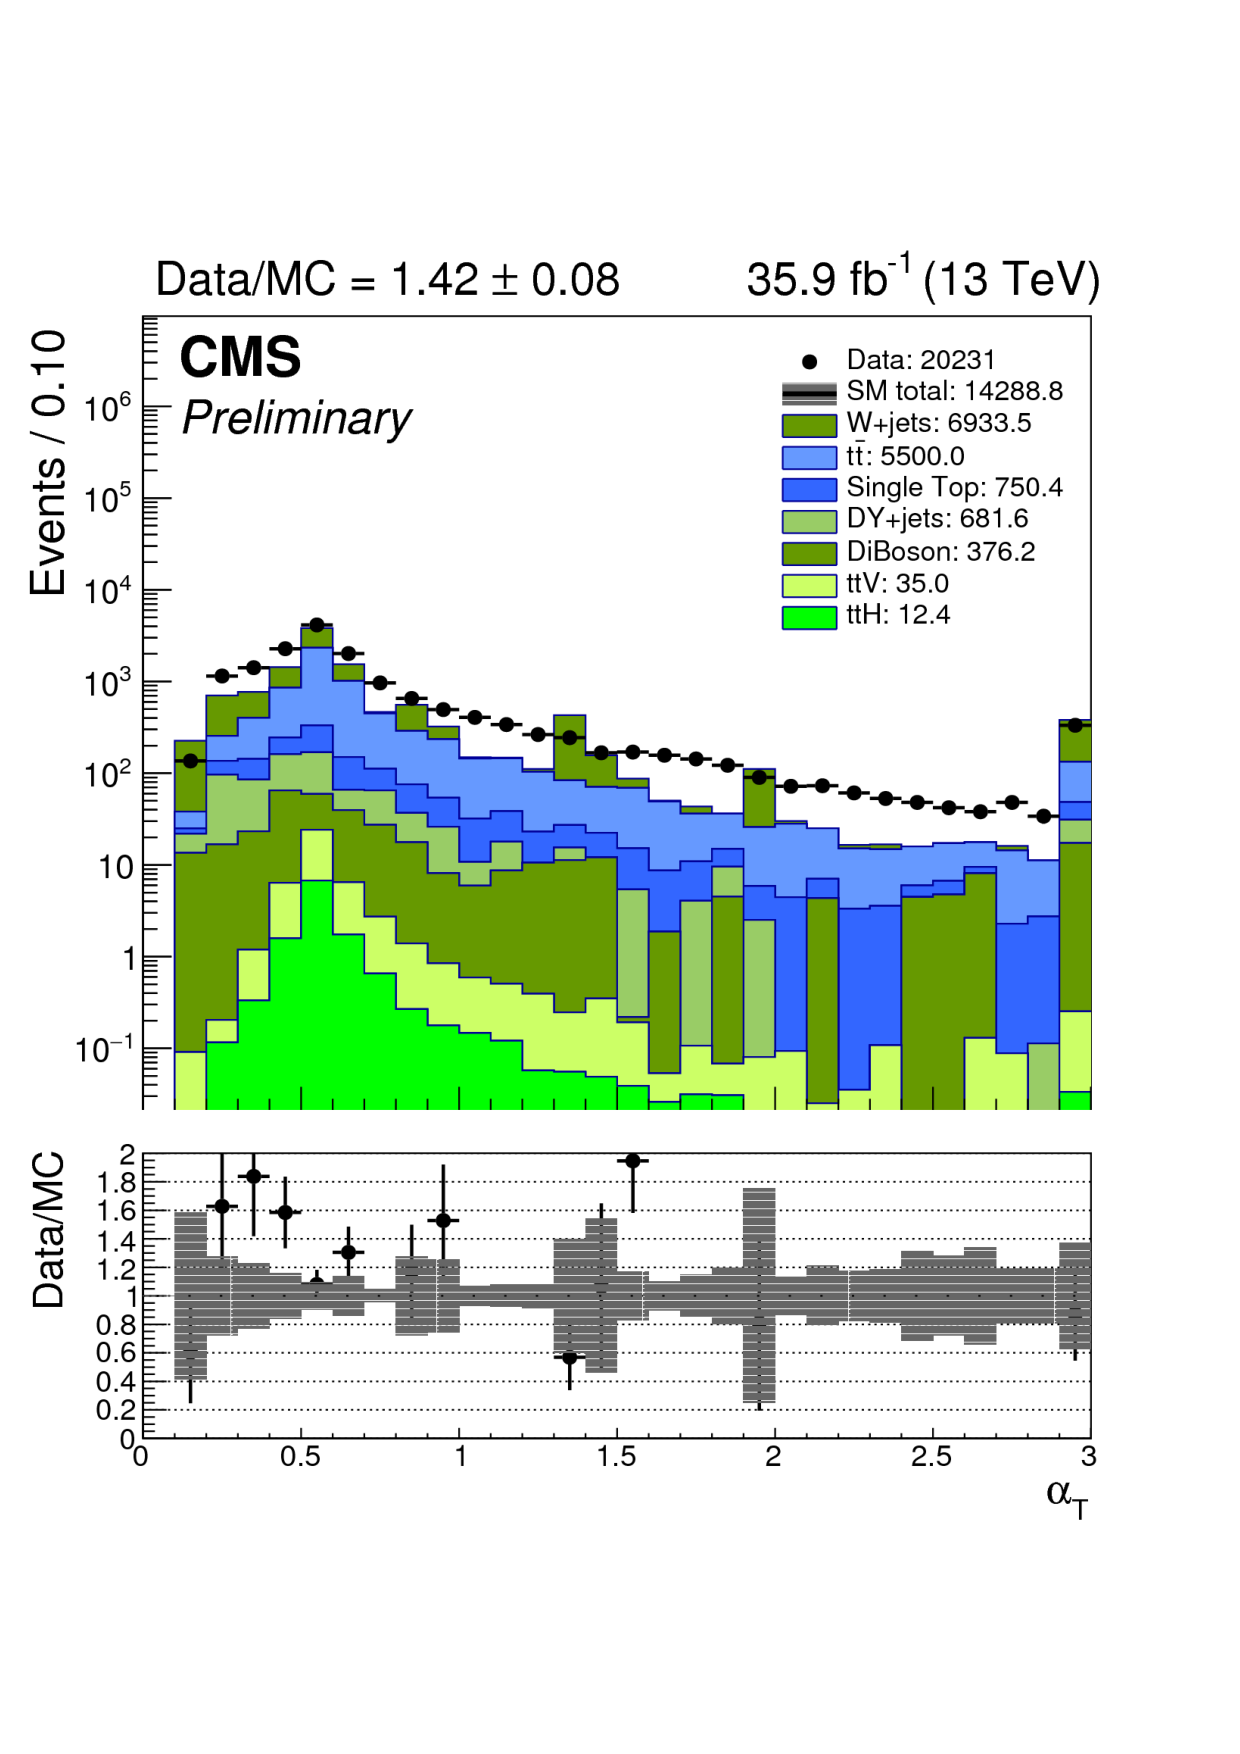
\includegraphics[width=0.3\textwidth,page=1,trim=0 100 50 100,clip]{figures/SITV/Event/Event.pdf}~
    \includegraphics[width=0.3\textwidth,page=2,trim=0 100 50 100,clip]{figures/SITV/Event/Event.pdf}\\
    \includegraphics[width=0.3\textwidth,page=11,trim=0 100 50 100,clip]{figures/SITV/Event/Event.pdf}~
    \includegraphics[width=0.3\textwidth,page=9,trim=0 100 50 100,clip]{figures/SITV/Event/Event.pdf}~
    \includegraphics[width=0.3\textwidth,page=12,trim=0 100 50 100,clip]{figures/SITV/Event/Event.pdf}\\
    \caption{Distributions of various event-level quantities within a
      sample of \mj events containing at least SIT.}
    \label{fig:dataMC_SITEvent_mu}
  \end{center} 
\end{figure}




%\subsection{Top $p_T$ reweighting}
%
%\begin{figure}[!h]
%  \centering
%  \subfigure[top $p_{T}$ weight up variation]{
%    \includegraphics[width=0.5\textwidth]{figures/mcSystematics36p4fb/Zinv/mu/ratiotfh_ht_mht_alltopPtWeight_Up.pdf}
%  } ~~
%  \subfigure[top $p_{T}$ weight down variation]{
%    \includegraphics[width=0.5\textwidth]{figures/mcSystematics36p4fb/Zinv/mu/ratiotfh_ht_mht_alltopPtWeight_Down.pdf}
%  }\\
%
%  \caption{\label{fig:tfSyst_topPt_muToZinv} The relative change in
%  the $\mj \rightarrow (\znunu)$ transfer
%  factors when varying top $p_{T}$ weight in MC within its uncertainties, as a function of \scalht and jet category. 
%  Variations corresponding to $+1\sigma$ ($-1\sigma$) are shown in the left (right) figure. 
%  }
%\end{figure}
%
%\begin{figure}[!h]
%  \centering
%  \subfigure[top $p_{T}$ weight up variation]{
%    \includegraphics[width=0.5\textwidth]{figures/mcSystematics36p4fb/Zinv/mumu/ratiotfh_ht_mht_alltopPtWeight_Up.pdf}
%  } ~~
%  \subfigure[top $p_{T}$ weight down variation]{
%    \includegraphics[width=0.5\textwidth]{figures/mcSystematics36p4fb/Zinv/mumu/ratiotfh_ht_mht_alltopPtWeight_Down.pdf}
%  }\\
%
%  \caption{\label{fig:tfSyst_topPt_mumuToZinv} The relative change in
%  the $\mmj \rightarrow (\znunu)$ transfer
%  factors when varying top $p_{T}$ weight in MC within its uncertainties, as a function of \scalht and jet category. 
%  Variations corresponding to $+1\sigma$ ($-1\sigma$) are shown in the left (right) figure. 
%  }
%\end{figure}
%
%\begin{figure}[!h]
%  \centering
%  \subfigure[top $p_{T}$ weight up variation]{
%    \includegraphics[width=0.5\textwidth]{figures/mcSystematics36p4fb/Ttw/mu/ratiotfh_ht_mht_alltopPtWeight_Up.pdf}
%  } ~~
%  \subfigure[top $p_{T}$ weight down variation]{
%    \includegraphics[width=0.5\textwidth]{figures/mcSystematics36p4fb/Ttw/mu/ratiotfh_ht_mht_alltopPtWeight_Down.pdf}
%  }\\
%
%  \caption{\label{fig:tfSyst_topPt_muToTtw} The relative change in the $\mj \rightarrow \mathrm{tt+W}$ transfer
%  factors when varying top $p_{T}$ weight in MC within its uncertainties, as a function of \scalht and jet category. 
%  Variations corresponding to $+1\sigma$ ($-1\sigma$) are shown in the left (right) figure. 
%  }
%\end{figure}

